\documentclass[a4paper,11pt]{article}
\usepackage[english]{babel}
\usepackage[utf8]{inputenc}
\usepackage{graphicx}
\usepackage{epstopdf}
\usepackage[labelfont=bf]{caption}
\usepackage{adjustbox}
\usepackage{float}
\usepackage{array}
\newcolumntype{M}[1]{>{\centering\arraybackslash}m{#1}}

\author{A.~Battistello\and P.~Ferretti}
\title{Machine Learning techniques to Model Data Intensive Application Performance}
\date{}
\begin{document}
\maketitle
\tableofcontents

%-----------------------------------------------

\newpage
\section{Fixed Datasize, All the Features}
\subsection{Query R1}
\subsubsection{Query R1 -- Datasize 250}
\begin{table}[H]
	\centering
	\begin{adjustbox}{center}
		\begin{tabular}{c | c M{1.2cm} M{2.5cm} M{2.5cm} M{1.8cm}}
			Model & RMSE & R\textsuperscript{2} & Mean absolute error & Mean relative error & Mean difference \tabularnewline
			\hline
			Linear regression & 0.3041 & 0.9591 &  57811 & 0.1197 & -0.1014 \\
			Linear SVR & 0.3418 & 0.9830 &  58151 & 0.1379 & -0.1117 \\
			Polynomial SVR (2) & 0.7566 & 0.7509 &  65973 & 5.1551 & 0.0961 \\
			Polynomial SVR (3) & 4.2307 & 0.7818 &  78538 & 0.9196 & 1.2843 \\
			Polynomial SVR (4) & 1.1959 & 0.4622 &  66397 & 2.9871 & -0.1070 \\
			Polynomial SVR (6) & 5.3772 & 0.4964 &  92865 & 10.5804 & 1.0027 \\
			Gaussian SVR & 1.2070 & 0.4548 &  63139 & 2.0853 & -0.3691 \\
		\end{tabular}
	\end{adjustbox}
	\\
	\caption{Results for R1-250}
	\label{fig:all_linear_R1_250}
\end{table}

\begin {figure}[hbtp]
\centering
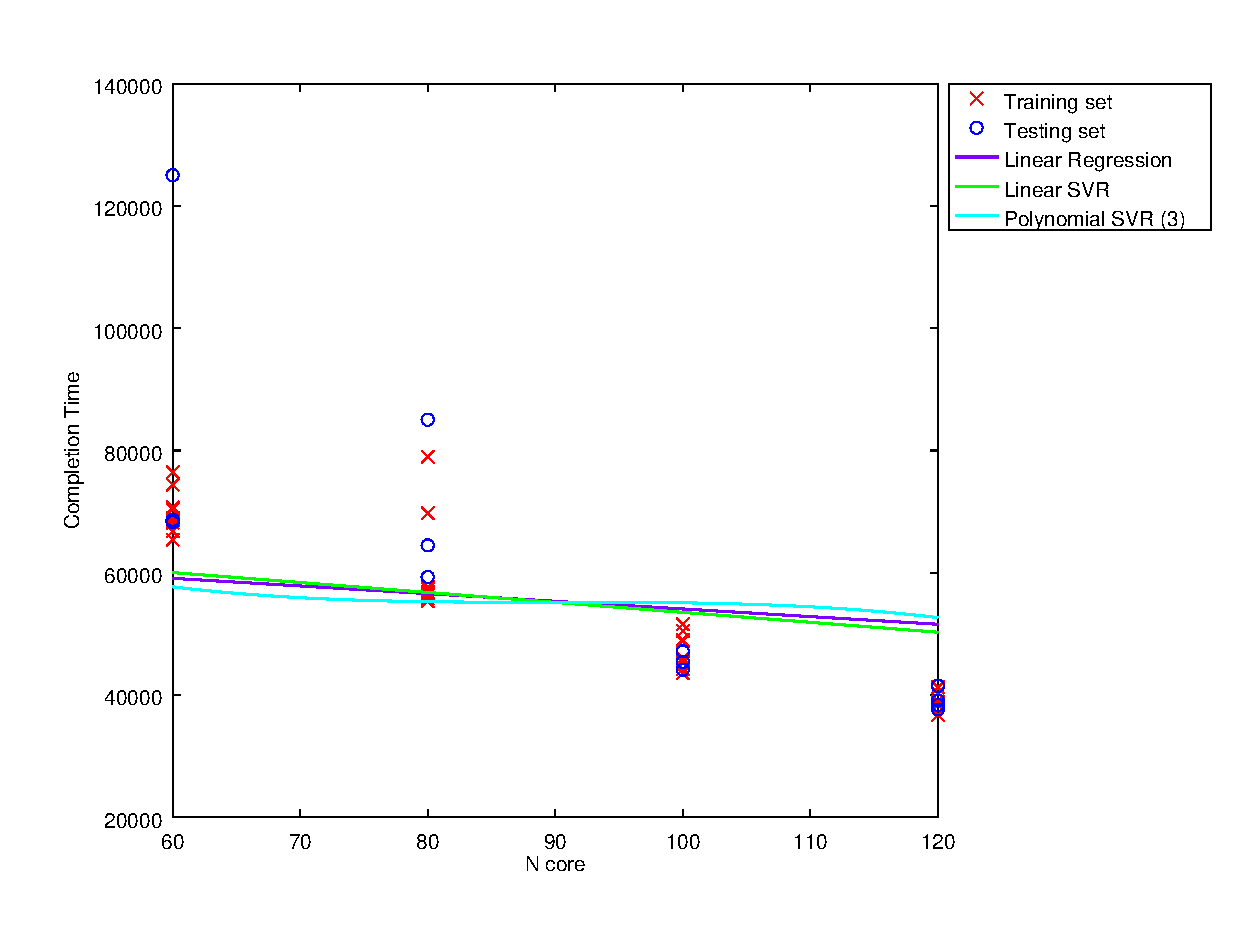
\includegraphics[width=\textwidth]{output/R1_250_LINEAR_NCORE/plot_R1_250_bestmodels.eps}
\caption{Completion time vs ncores for query R1 with datasize 250}
\label{fig:all_linear_R1_250}
\end {figure}

\newpage
\subsubsection{Query R1 -- Datasize 500}
\begin{table}[H]
	\centering
	\begin{adjustbox}{center}
		\begin{tabular}{c | c M{1.2cm} M{2.5cm} M{2.5cm} M{1.8cm}}
			Model & RMSE & R\textsuperscript{2} & Mean absolute error & Mean relative error & Mean difference \tabularnewline
			\hline
			Linear regression & 0.0542 & 0.9938 & 149334 & 0.1271 & -0.0207 \\
			Linear SVR & 0.0751 & 0.9895 & 151476 & 0.2409 & -0.0116 \\
			Polynomial SVR (2) & 0.4332 & 0.6640 & 169212 & 1.0417 & -0.0427 \\
			Polynomial SVR (3) & 0.3357 & 0.8853 & 163273 & 0.5244 & -0.0205 \\
			Polynomial SVR (4) & 0.5014 & 0.6016 & 169259 & 1.0401 & -0.0484 \\
			Polynomial SVR (6) & 0.5554 & 0.4560 & 172257 & 2.6883 & -0.0169 \\
			Gaussian SVR & 0.3650 & 0.8383 & 162324 & 0.8210 & -0.0202 \\
		\end{tabular}
	\end{adjustbox}
	\\
	\caption{Results for R1-500}
	\label{fig:all_linear_R1_500}
\end{table}

\begin {figure}[hbtp]
\centering
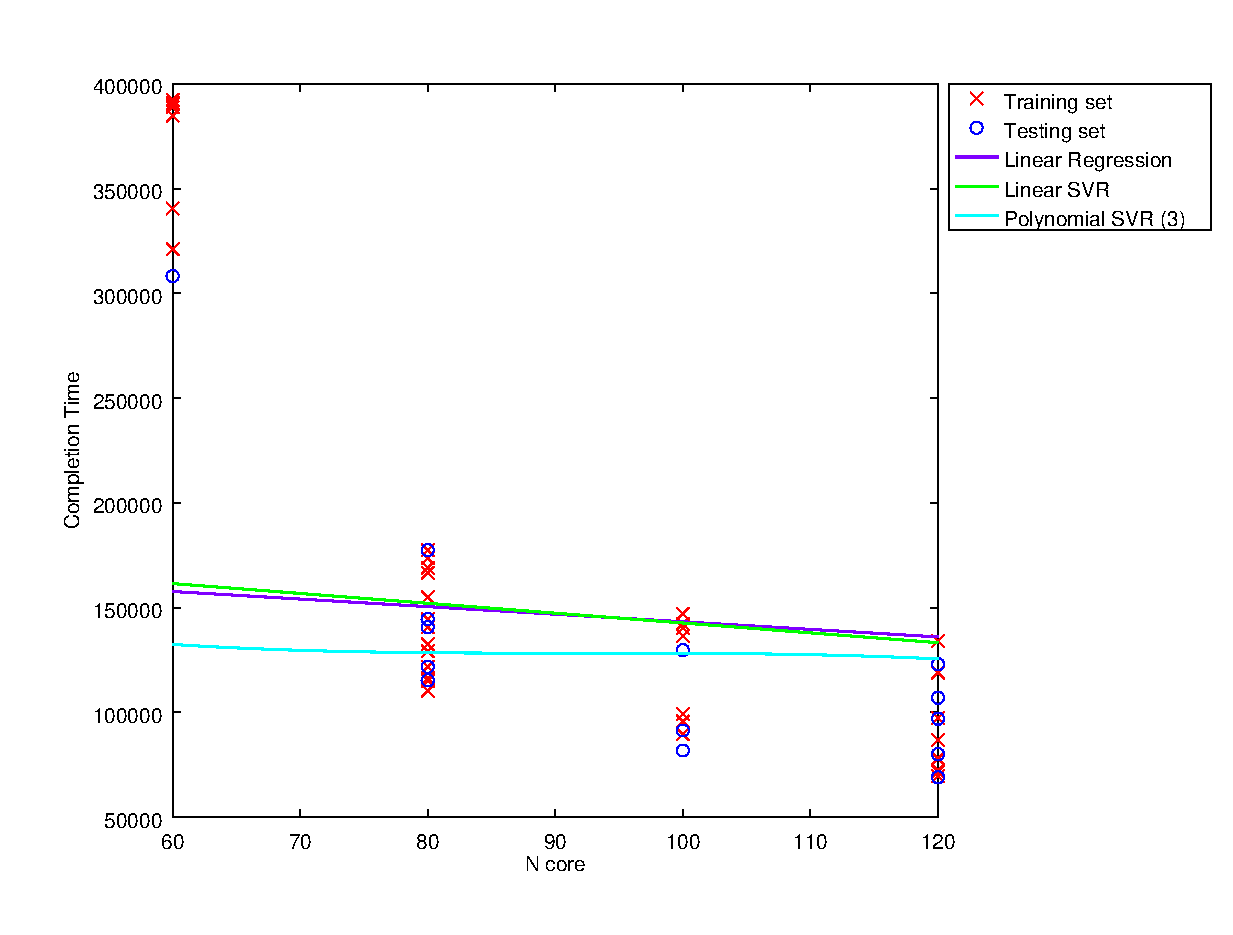
\includegraphics[width=\textwidth]{output/R1_500_LINEAR_NCORE/plot_R1_500_bestmodels.eps}
\caption{Completion time vs ncores for query R1 with datasize 500}
\label{fig:all_linear_R1_500}
\end {figure}

\newpage
\subsubsection{Query R1 -- Datasize 750}
\begin{table}[H]
	\centering
	\begin{adjustbox}{center}
		\begin{tabular}{c | c M{1.2cm} M{2.5cm} M{2.5cm} M{1.8cm}}
			Model & RMSE & R\textsuperscript{2} & Mean absolute error & Mean relative error & Mean difference \tabularnewline
			\hline
			Linear regression & 0.1572 & 0.9665 & 266884 & 0.1727 & 0.0236 \\
			Linear SVR & 0.2120 & 0.9688 & 272955 & 0.2542 & 0.1291 \\
			Polynomial SVR (2) & 0.7508 & 0.3524 & 315378 & 3.4186 & 0.2712 \\
			Polynomial SVR (3) & 0.3593 & 0.9177 & 283626 & 0.7417 & 0.0705 \\
			Polynomial SVR (4) & 0.7471 & 0.3213 & 313379 & 60.2071 & 0.1553 \\
			Polynomial SVR (6) & 0.7398 & 0.3099 & 312928 & 72.9881 & 0.1585 \\
			Gaussian SVR & 0.2646 & 0.9347 & 275101 & 0.3102 & 0.1353 \\
		\end{tabular}
	\end{adjustbox}
	\\
	\caption{Results for R1-750}
	\label{fig:all_linear_R1_750}
\end{table}

\begin {figure}[hbtp]
\centering
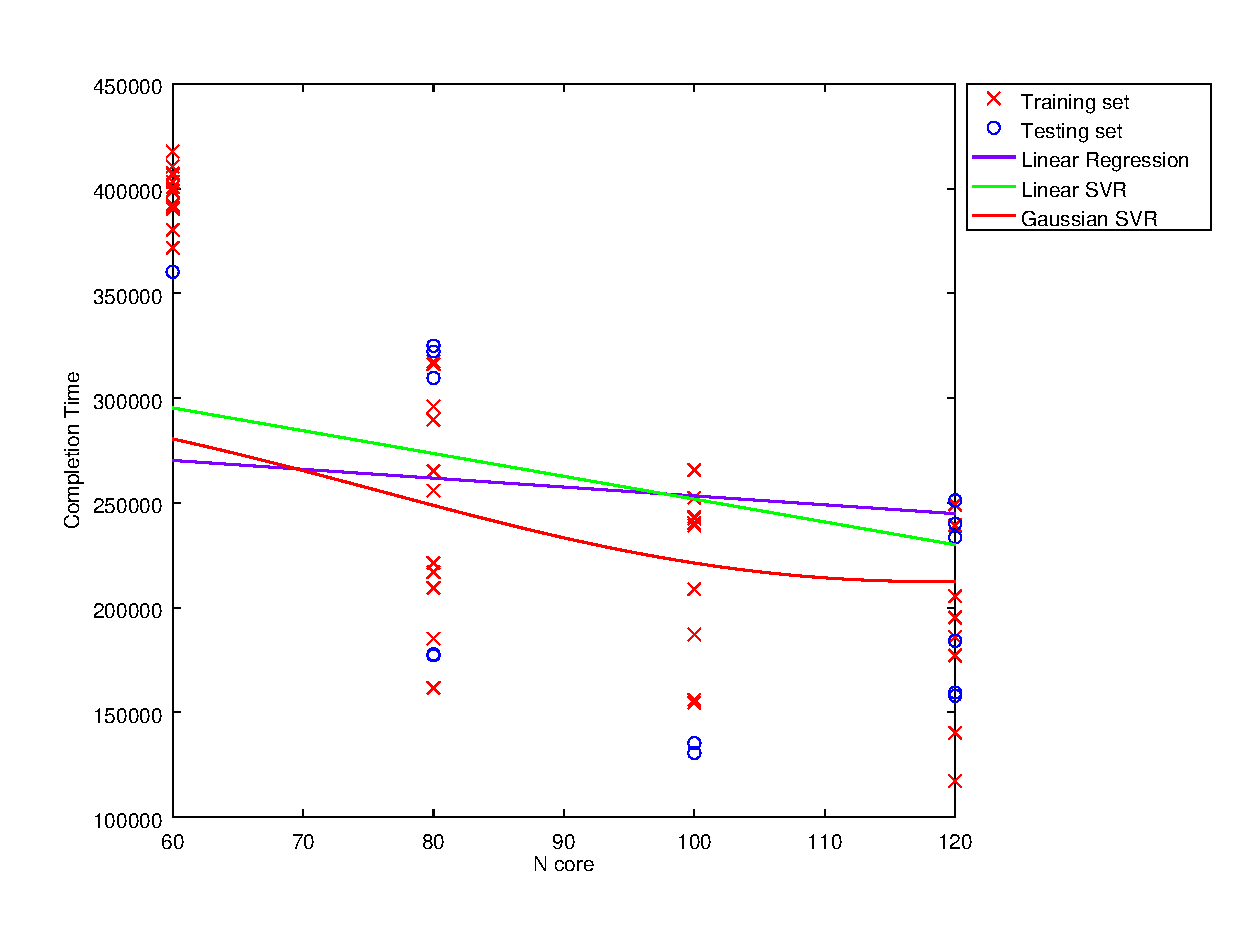
\includegraphics[width=\textwidth]{output/R1_750_LINEAR_NCORE/plot_R1_750_bestmodels.eps}
\caption{Completion time vs ncores for query R1 with datasize 750}
\label{fig:all_linear_R1_750}
\end {figure}

\newpage
\subsubsection{Query R1 -- Datasize 1000}
\begin{table}[H]
	\centering
	\begin{adjustbox}{center}
		\begin{tabular}{c | c M{1.2cm} M{2.5cm} M{2.5cm} M{1.8cm}}
			Model & RMSE & R\textsuperscript{2} & Mean absolute error & Mean relative error & Mean difference \tabularnewline
			\hline
			Linear regression & 0.1415 & 0.9746 & 428799 & 12.4975 & 0.0202 \\
			Linear SVR & 0.1468 & 0.9778 & 429594 & 0.4042 & 0.0313 \\
			Polynomial SVR (2) & 0.8789 & 0.1424 & 485672 & 6.3522 & 0.1723 \\
			Polynomial SVR (3) & 1.0942 & 0.6134 & 471899 & 0.9966 & -0.3248 \\
			Polynomial SVR (4) & 0.9412 & 0.1817 & 478644 & 1.5192 & 0.2905 \\
			Polynomial SVR (6) & 4.8069 & 0.0294 & 603664 & 0.9923 & 1.7839 \\
			Gaussian SVR & 0.4428 & 0.8139 & 442219 & 5.7558 & 0.2039 \\
		\end{tabular}
	\end{adjustbox}
	\\
	\caption{Results for R1-1000}
	\label{fig:all_linear_R1_1000}
\end{table}

\begin {figure}[hbtp]
\centering
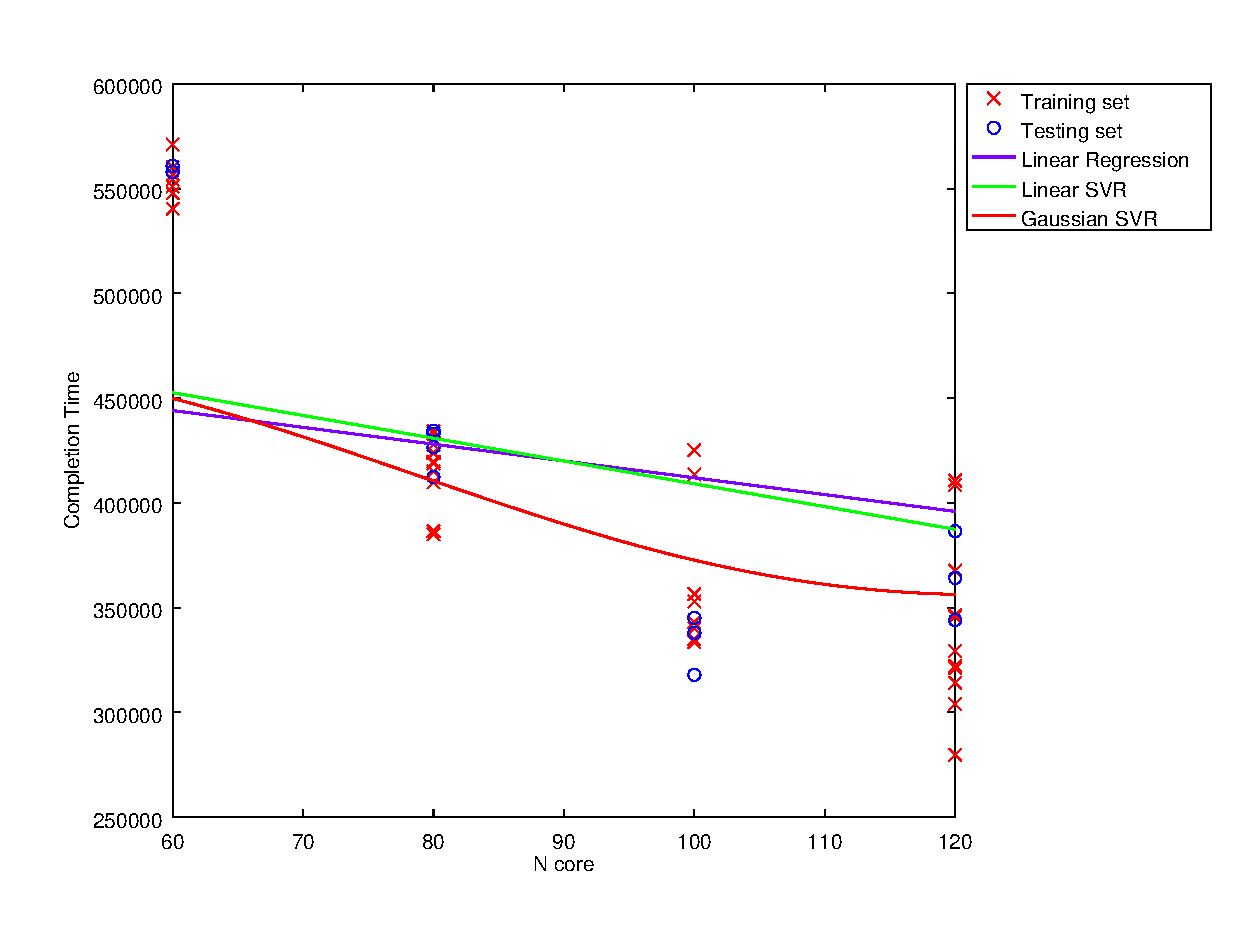
\includegraphics[width=\textwidth]{output/R1_1000_LINEAR_NCORE/plot_R1_1000_bestmodels.eps}
\caption{Completion time vs ncores for query R1 with datasize 1000}
\label{fig:all_linear_R1_1000}
\end {figure}

\newpage
\subsection{Query R2}
\subsubsection{Query R2 -- Datasize 250}
\begin{table}[H]
	\centering
	\begin{adjustbox}{center}
		\begin{tabular}{c | c M{1.2cm} M{2.5cm} M{2.5cm} M{1.8cm}}
			Model & RMSE & R\textsuperscript{2} & Mean absolute error & Mean relative error & Mean difference \tabularnewline
			\hline
			Linear regression & 0.2833 & 0.8674 &  83142 & 0.6094 & 0.1530 \\
			Linear SVR & 0.2360 & 0.9197 &  83061 & 0.9073 & 0.0259 \\
			Polynomial SVR (2) & 0.9310 & 0.0443 &  84553 & 3.0651 & 0.1369 \\
			Polynomial SVR (3) & 0.6599 & 0.6297 &  83769 & 6.0596 & 0.2908 \\
			Polynomial SVR (4) & 0.7044 & 0.5309 &  84118 & 4.1167 & 0.2338 \\
			Polynomial SVR (6) & 0.7484 & 0.4866 &  84168 & 14.5076 & 0.0498 \\
			Gaussian SVR & 0.3253 & 0.8273 &  83303 & 0.6058 & 0.0159 \\
		\end{tabular}
	\end{adjustbox}
	\\
	\caption{Results for R2-250}
	\label{fig:all_linear_R2_250}
\end{table}

\begin {figure}[hbtp]
\centering
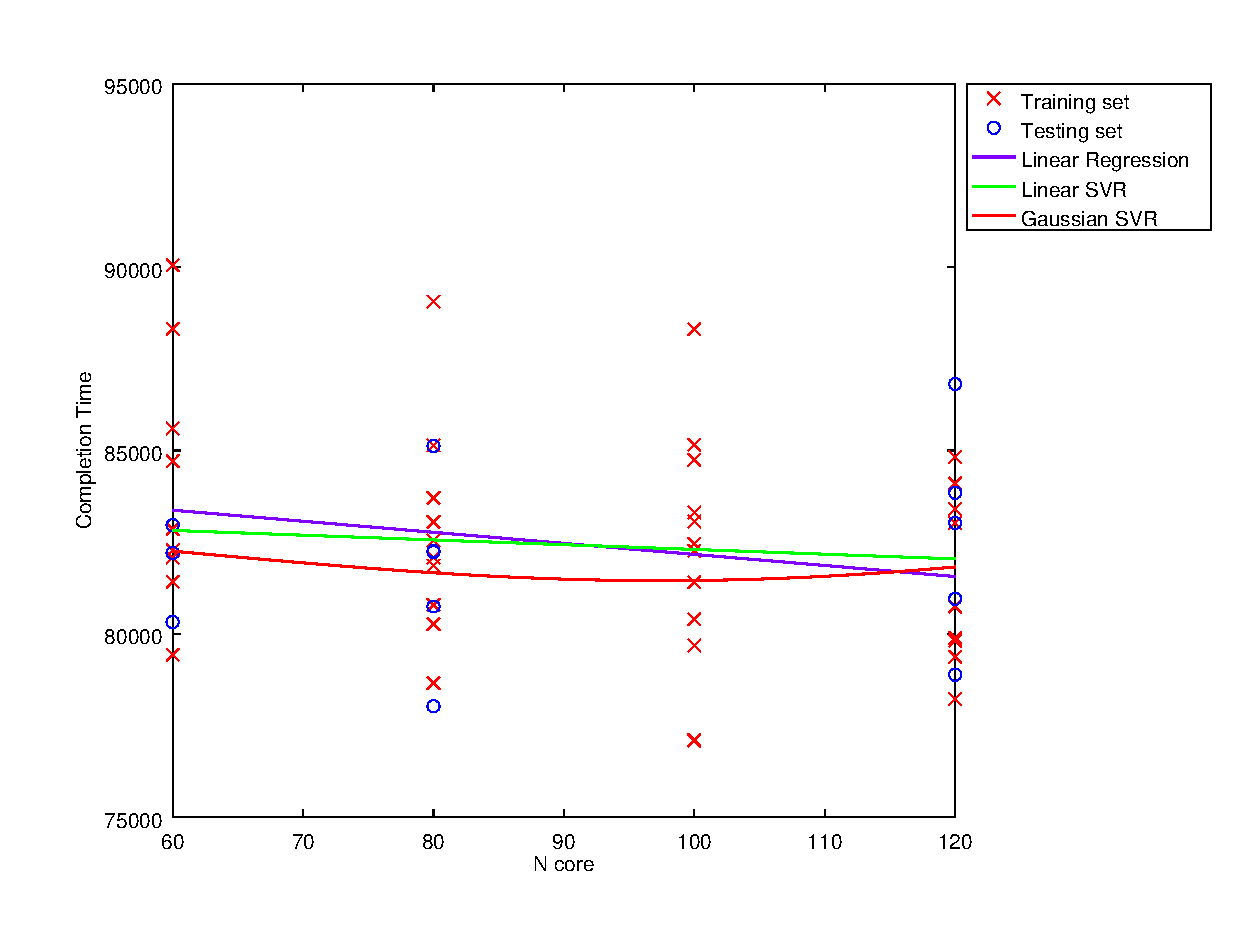
\includegraphics[width=\textwidth]{output/R2_250_LINEAR_NCORE/plot_R2_250_bestmodels.eps}
\caption{Completion time vs ncores for query R2 with datasize 250}
\label{fig:all_linear_R2_250}
\end {figure}

\newpage
\subsubsection{Query R2 -- Datasize 500}
\begin{table}[H]
	\centering
	\begin{adjustbox}{center}
		\begin{tabular}{c | c M{1.2cm} M{2.5cm} M{2.5cm} M{1.8cm}}
			Model & RMSE & R\textsuperscript{2} & Mean absolute error & Mean relative error & Mean difference \tabularnewline
			\hline
			Linear regression & 0.2486 & 0.9587 &  73222 & 0.5333 & -0.0463 \\
			Linear SVR & 0.2416 & 0.9633 &  73182 & 0.4394 & -0.0307 \\
			Polynomial SVR (2) & 2.2423 & 0.0470 &  76750 & 2.9641 & -0.1625 \\
			Polynomial SVR (3) & 4.4063 & 0.3043 &  77823 & 2.0078 & 0.9745 \\
			Polynomial SVR (4) & 1.6306 & 0.0087 &  76066 & 15.9898 & -0.2811 \\
			Polynomial SVR (6) & 1.3874 & 0.0000 &  75520 & 3.6901 & -0.6539 \\
			Gaussian SVR & 0.7416 & 0.7166 &  74076 & 3.4206 & -0.2667 \\
		\end{tabular}
	\end{adjustbox}
	\\
	\caption{Results for R2-500}
	\label{fig:all_linear_R2_500}
\end{table}

\begin {figure}[hbtp]
\centering
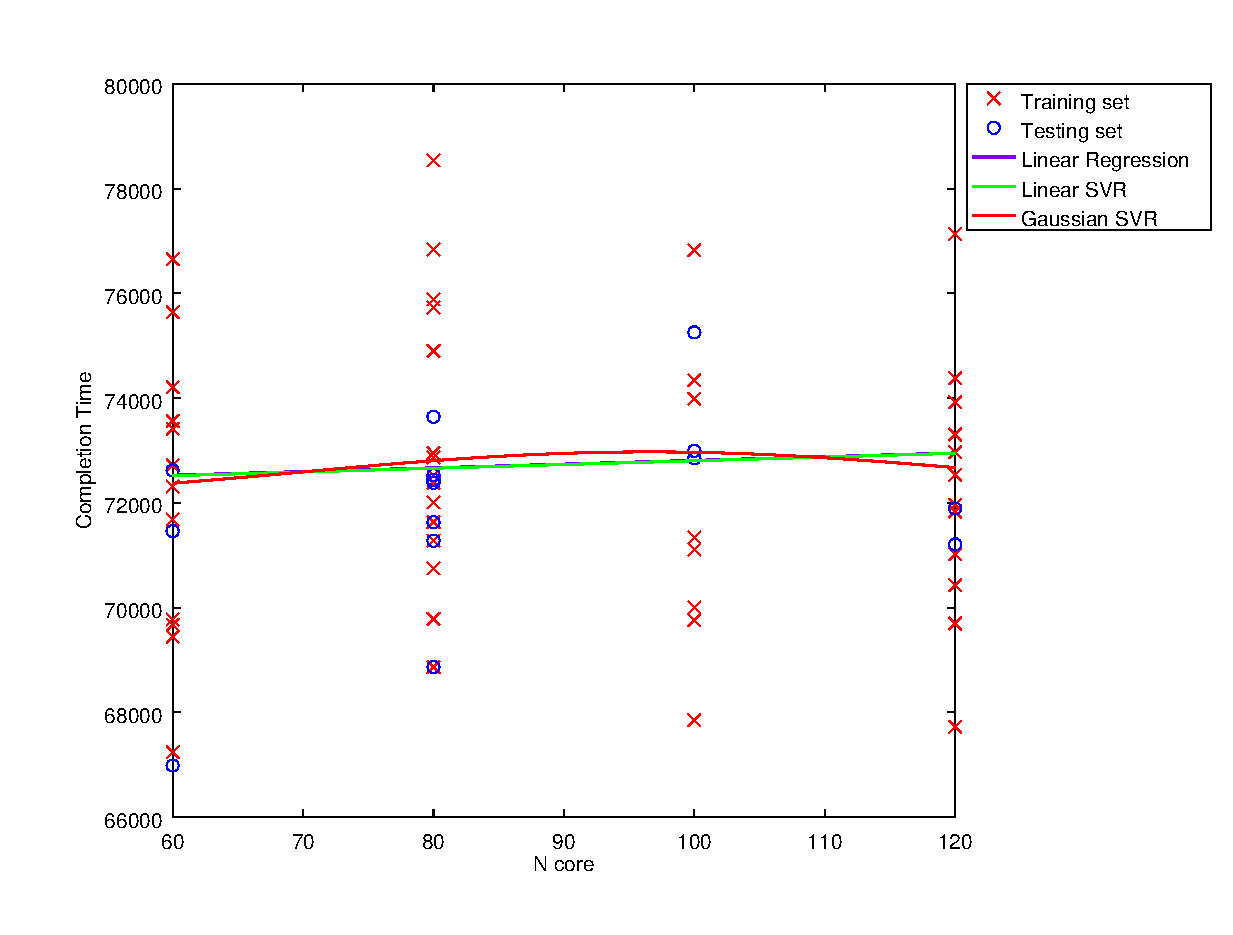
\includegraphics[width=\textwidth]{output/R2_500_LINEAR_NCORE/plot_R2_500_bestmodels.eps}
\caption{Completion time vs ncores for query R2 with datasize 500}
\label{fig:all_linear_R2_500}
\end {figure}

\newpage
\subsubsection{Query R2 -- Datasize 750}
\begin{table}[H]
	\centering
	\begin{adjustbox}{center}
		\begin{tabular}{c | c M{1.2cm} M{2.5cm} M{2.5cm} M{1.8cm}}
			Model & RMSE & R\textsuperscript{2} & Mean absolute error & Mean relative error & Mean difference \tabularnewline
			\hline
			Linear regression & 0.2218 & 0.9212 &  78832 & 0.9479 & 0.0374 \\
			Linear SVR & 0.2474 & 0.9477 &  78888 & 1.5734 & 0.0137 \\
			Polynomial SVR (2) & 0.8172 & 0.2052 &  79812 & 6.7278 & -0.0623 \\
			Polynomial SVR (3) & 0.5008 & 0.7150 &  79358 & 3.0113 & -0.0459 \\
			Polynomial SVR (4) & 0.8079 & -0.0000 &  79779 & 3.1582 & -0.1683 \\
			Polynomial SVR (6) & 0.8079 & -0.0000 &  79779 & 3.1582 & -0.1683 \\
			Gaussian SVR & 0.4815 & 0.7359 &  79228 & 2.3664 & 0.1155 \\
		\end{tabular}
	\end{adjustbox}
	\\
	\caption{Results for R2-750}
	\label{fig:all_linear_R2_750}
\end{table}

\begin {figure}[hbtp]
\centering
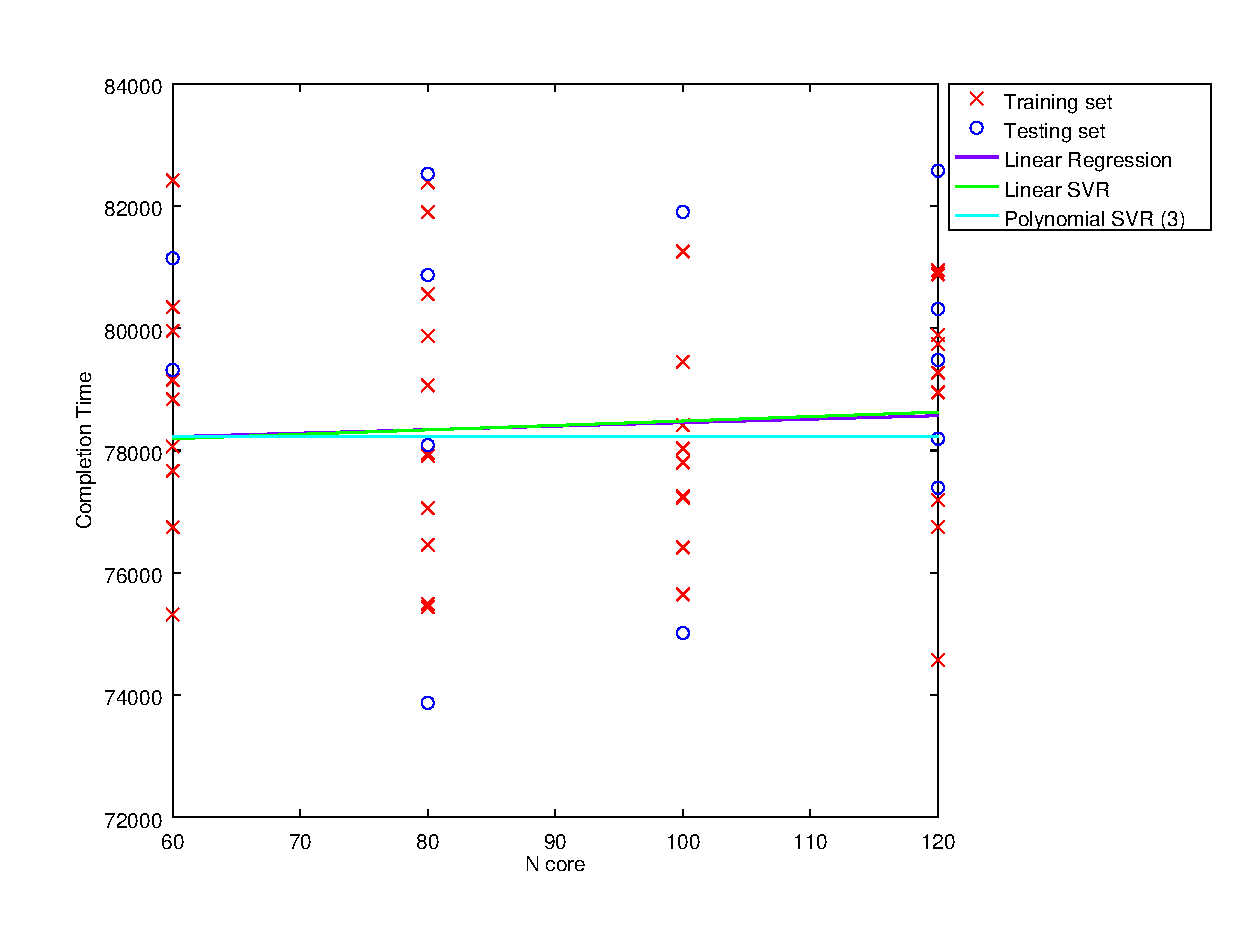
\includegraphics[width=\textwidth]{output/R2_750_LINEAR_NCORE/plot_R2_750_bestmodels.eps}
\caption{Completion time vs ncores for query R2 with datasize 750}
\label{fig:all_linear_R2_750}
\end {figure}

\newpage
\subsubsection{Query R2 -- Datasize 1000}
\begin{table}[H]
	\centering
	\begin{adjustbox}{center}
		\begin{tabular}{c | c M{1.2cm} M{2.5cm} M{2.5cm} M{1.8cm}}
			Model & RMSE & R\textsuperscript{2} & Mean absolute error & Mean relative error & Mean difference \tabularnewline
			\hline
			Linear regression & 0.0461 & 0.9983 & 1123883 & 0.1832 & 0.0106 \\
			Linear SVR & 0.0795 & 0.9955 & 1140986 & 0.2159 & -0.0181 \\
			Polynomial SVR (2) & 0.7956 & 0.5804 & 1491974 & 8.3707 & 0.0548 \\
			Polynomial SVR (3) & 0.4919 & 0.9200 & 1280834 & 0.6962 & 0.1826 \\
			Polynomial SVR (4) & 0.8016 & 0.6890 & 1454684 & 2.8509 & 0.3630 \\
			Polynomial SVR (6) & 0.5958 & 0.7861 & 1386601 & 3.8379 & 0.2563 \\
			Gaussian SVR & 0.2389 & 0.9715 & 1180539 & 0.3227 & -0.0662 \\
		\end{tabular}
	\end{adjustbox}
	\\
	\caption{Results for R2-1000}
	\label{fig:all_linear_R2_1000}
\end{table}

\begin {figure}[hbtp]
\centering
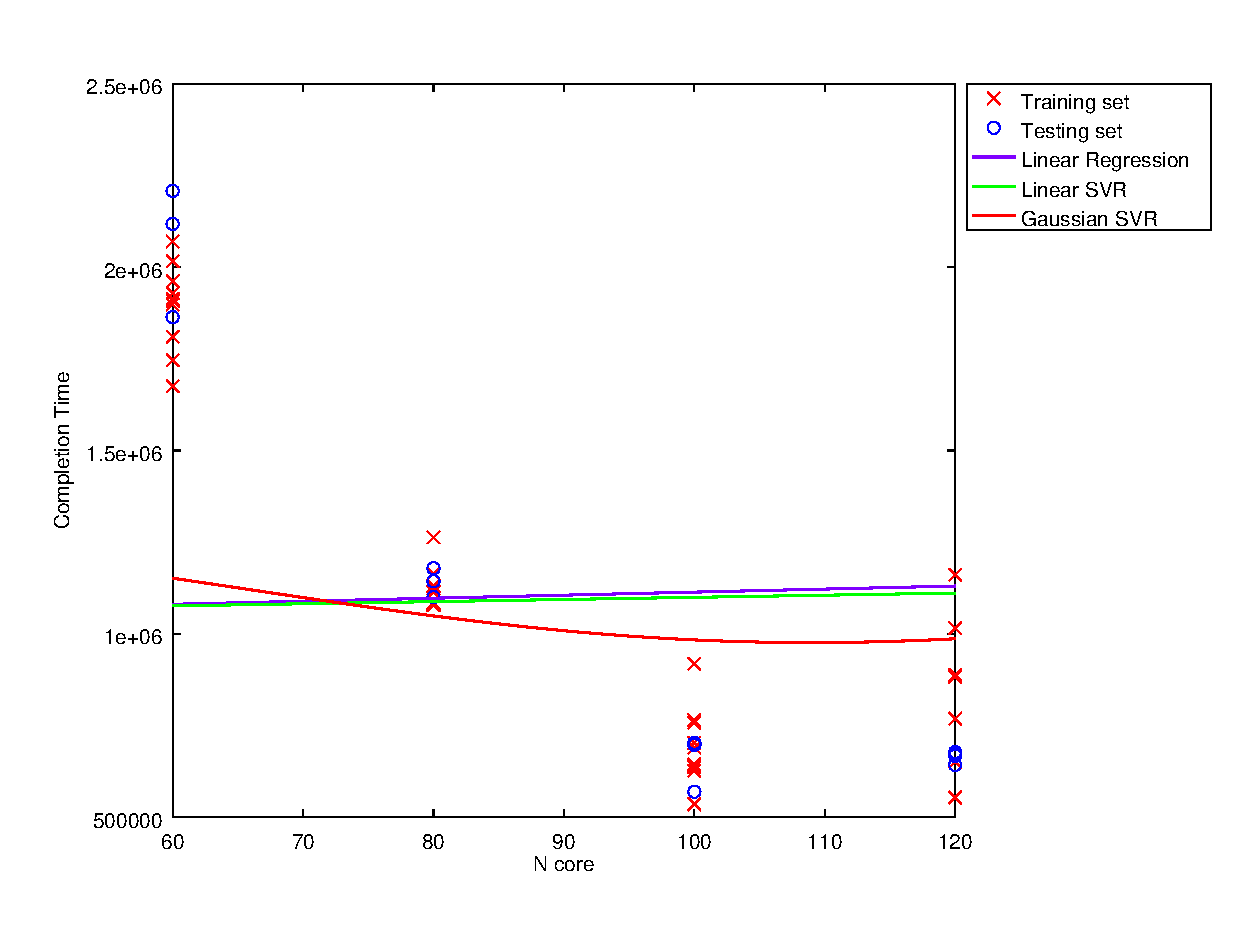
\includegraphics[width=\textwidth]{output/R2_1000_LINEAR_NCORE/plot_R2_1000_bestmodels.eps}
\caption{Completion time vs ncores for query R2 with datasize 1000}
\label{fig:all_linear_R2_1000}
\end {figure}

\newpage
\subsection{Query R3}
\subsubsection{Query R3 -- Datasize 250}
\begin{table}[H]
	\centering
	\begin{adjustbox}{center}
		\begin{tabular}{c | c M{1.2cm} M{2.5cm} M{2.5cm} M{1.8cm}}
			Model & RMSE & R\textsuperscript{2} & Mean absolute error & Mean relative error & Mean difference \tabularnewline
			\hline
			Linear regression & 0.2164 & 0.9356 & 189440 & 0.1617 & -0.0659 \\
			Linear SVR & 0.1819 & 0.9594 & 190378 & 0.2102 & -0.0492 \\
			Polynomial SVR (2) & 0.7504 & 0.3004 & 226788 & 2.4661 & -0.2155 \\
			Polynomial SVR (3) & 0.5266 & 0.8156 & 211407 & 11.8470 & -0.0840 \\
			Polynomial SVR (4) & 1.1775 & 0.0110 & 230749 & 2.6098 & 0.2008 \\
			Polynomial SVR (6) & 0.7168 & 0.3378 & 223057 & 15.8449 & -0.1608 \\
			Gaussian SVR & 0.3876 & 0.8415 & 198753 & 0.6241 & 0.0112 \\
		\end{tabular}
	\end{adjustbox}
	\\
	\caption{Results for R3-250}
	\label{fig:all_linear_R3_250}
\end{table}

\begin {figure}[hbtp]
\centering
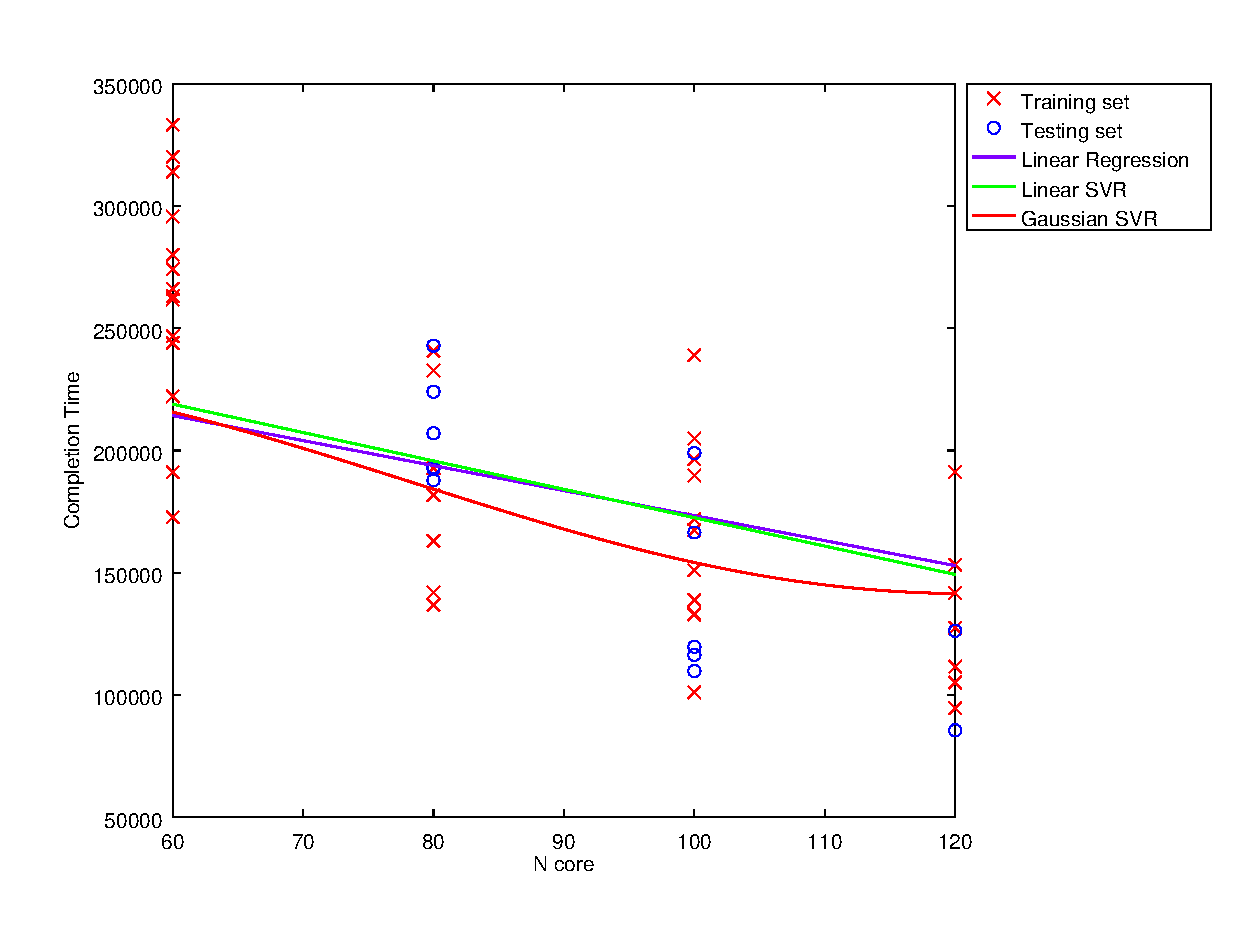
\includegraphics[width=\textwidth]{output/R3_250_LINEAR_NCORE/plot_R3_250_bestmodels.eps}
\caption{Completion time vs ncores for query R3 with datasize 250}
\label{fig:all_linear_R3_250}
\end {figure}

\newpage
\subsubsection{Query R3 -- Datasize 500}
\begin{table}[H]
	\centering
	\begin{adjustbox}{center}
		\begin{tabular}{c | c M{1.2cm} M{2.5cm} M{2.5cm} M{1.8cm}}
			Model & RMSE & R\textsuperscript{2} & Mean absolute error & Mean relative error & Mean difference \tabularnewline
			\hline
			Linear regression & 0.0510 & 0.9978 & 586577 & 0.0743 & -0.0177 \\
			Linear SVR & 0.0672 & 0.9981 & 591662 & 0.0863 & -0.0430 \\
			Polynomial SVR (2) & 0.5754 & 0.7757 & 704864 & 0.7898 & -0.1907 \\
			Polynomial SVR (3) & 0.2858 & 0.9404 & 645340 & 0.7538 & -0.0068 \\
			Polynomial SVR (4) & 0.4466 & 0.9154 & 681401 & 0.7641 & -0.0798 \\
			Polynomial SVR (6) & 0.5459 & 0.8250 & 699037 & 1.0813 & -0.0932 \\
			Gaussian SVR & 0.1400 & 0.9840 & 605179 & 93.5190 & -0.0230 \\
		\end{tabular}
	\end{adjustbox}
	\\
	\caption{Results for R3-500}
	\label{fig:all_linear_R3_500}
\end{table}

\begin {figure}[hbtp]
\centering
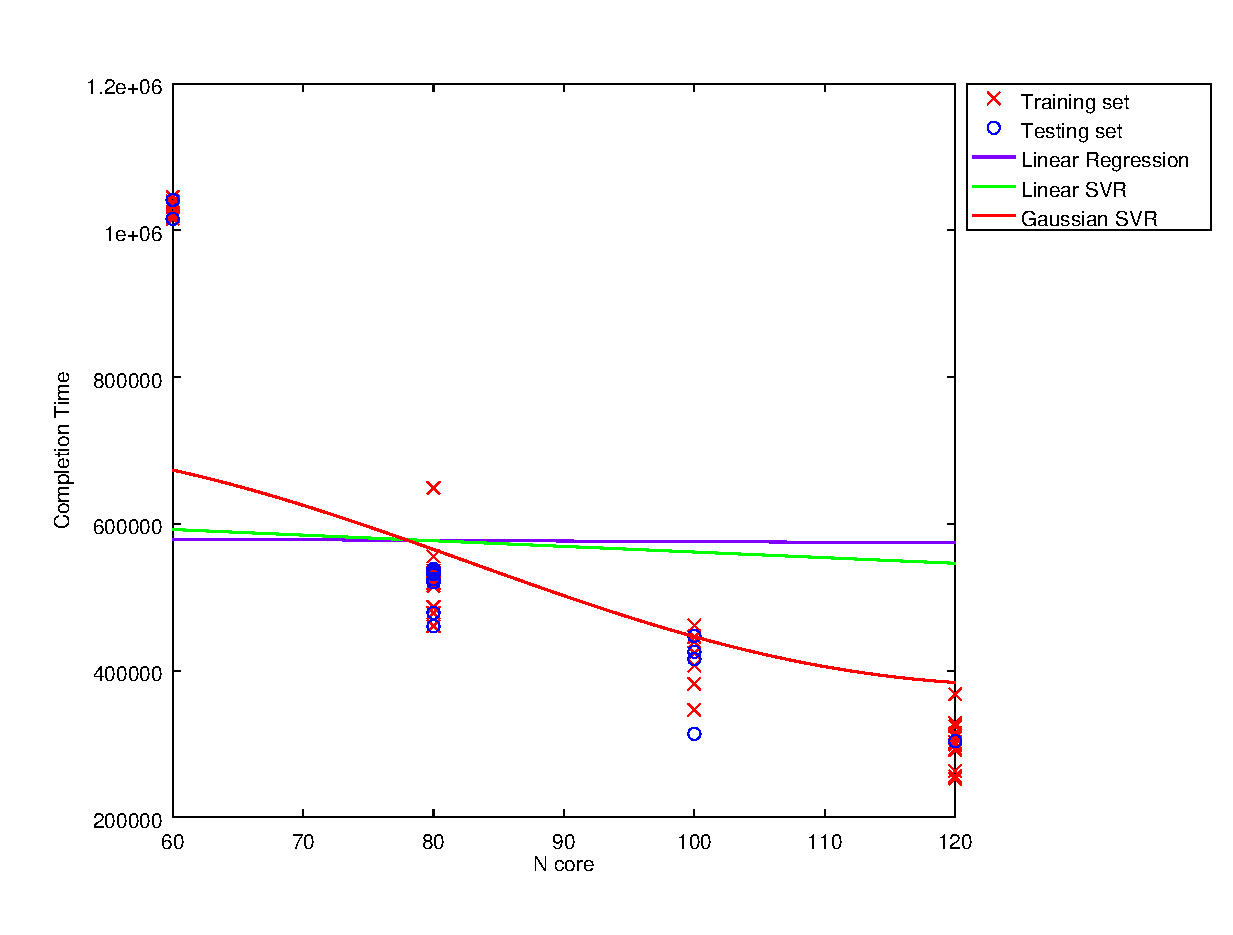
\includegraphics[width=\textwidth]{output/R3_500_LINEAR_NCORE/plot_R3_500_bestmodels.eps}
\caption{Completion time vs ncores for query R3 with datasize 500}
\label{fig:all_linear_R3_500}
\end {figure}

\newpage
\subsubsection{Query R3 -- Datasize 750}
\begin{table}[H]
	\centering
	\begin{adjustbox}{center}
		\begin{tabular}{c | c M{1.2cm} M{2.5cm} M{2.5cm} M{1.8cm}}
			Model & RMSE & R\textsuperscript{2} & Mean absolute error & Mean relative error & Mean difference \tabularnewline
			\hline
			Linear regression & 0.0194 & 0.9996 & 777482 & 0.1082 & -0.0036 \\
			Linear SVR & 0.0993 & 0.9928 & 790154 & 0.2445 & 0.0098 \\
			Polynomial SVR (2) & 0.6979 & 0.5785 & 872326 & 1.1036 & -0.0927 \\
			Polynomial SVR (3) & 0.3900 & 0.8646 & 826245 & 1.0606 & -0.0070 \\
			Polynomial SVR (4) & 0.6745 & 0.6525 & 871989 & 1.9560 & 0.0237 \\
			Polynomial SVR (6) & 0.7360 & 0.6058 & 878198 & 2.6868 & -0.0398 \\
			Gaussian SVR & 0.2505 & 0.9566 & 804169 & 0.4213 & 0.1072 \\
		\end{tabular}
	\end{adjustbox}
	\\
	\caption{Results for R3-750}
	\label{fig:all_linear_R3_750}
\end{table}

\begin {figure}[hbtp]
\centering
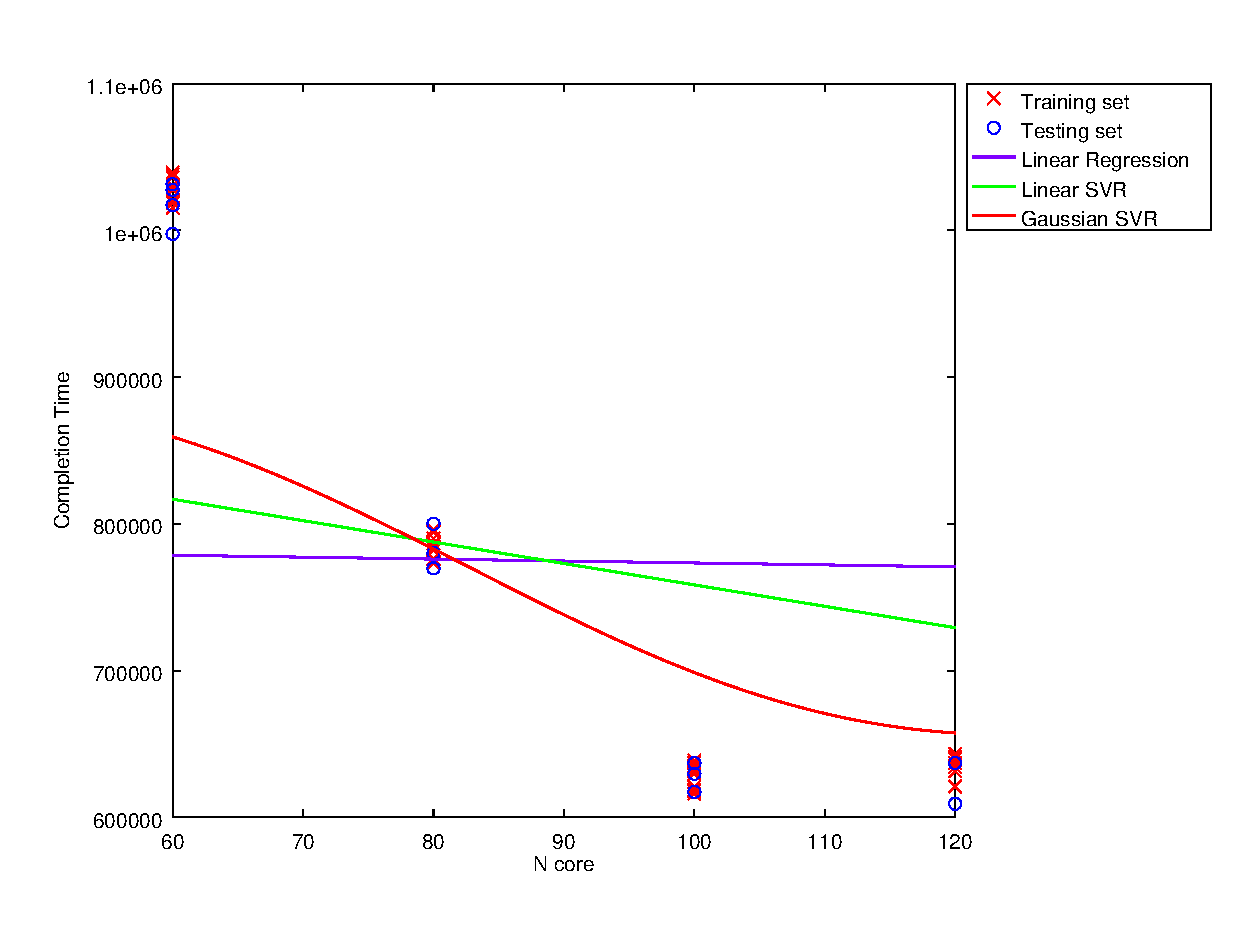
\includegraphics[width=\textwidth]{output/R3_750_LINEAR_NCORE/plot_R3_750_bestmodels.eps}
\caption{Completion time vs ncores for query R3 with datasize 750}
\label{fig:all_linear_R3_750}
\end {figure}

\newpage
\subsubsection{Query R3 -- Datasize 1000}
\begin{table}[H]
	\centering
	\begin{adjustbox}{center}
		\begin{tabular}{c | c M{1.2cm} M{2.5cm} M{2.5cm} M{1.8cm}}
			Model & RMSE & R\textsuperscript{2} & Mean absolute error & Mean relative error & Mean difference \tabularnewline
			\hline
			Linear regression & 0.0992 & 0.9903 & 1030310 & 0.4165 & -0.0382 \\
			Linear SVR & 0.1375 & 0.9868 & 1045712 & 0.4131 & -0.0644 \\
			Polynomial SVR (2) & 0.9305 & 0.1595 & 1201890 & 19.7317 & 0.0096 \\
			Polynomial SVR (3) & 0.5255 & 0.8592 & 1092985 & 0.5579 & -0.1767 \\
			Polynomial SVR (4) & 1.0806 & 0.0030 & 1216549 & 10.6991 & -0.0933 \\
			Polynomial SVR (6) & 1.1681 & 0.0031 & 1221010 & 6.4095 & -0.1238 \\
			Gaussian SVR & 0.4074 & 0.8877 & 1087163 & 1.5362 & -0.0031 \\
		\end{tabular}
	\end{adjustbox}
	\\
	\caption{Results for R3-1000}
	\label{fig:all_linear_R3_1000}
\end{table}

\begin {figure}[hbtp]
\centering
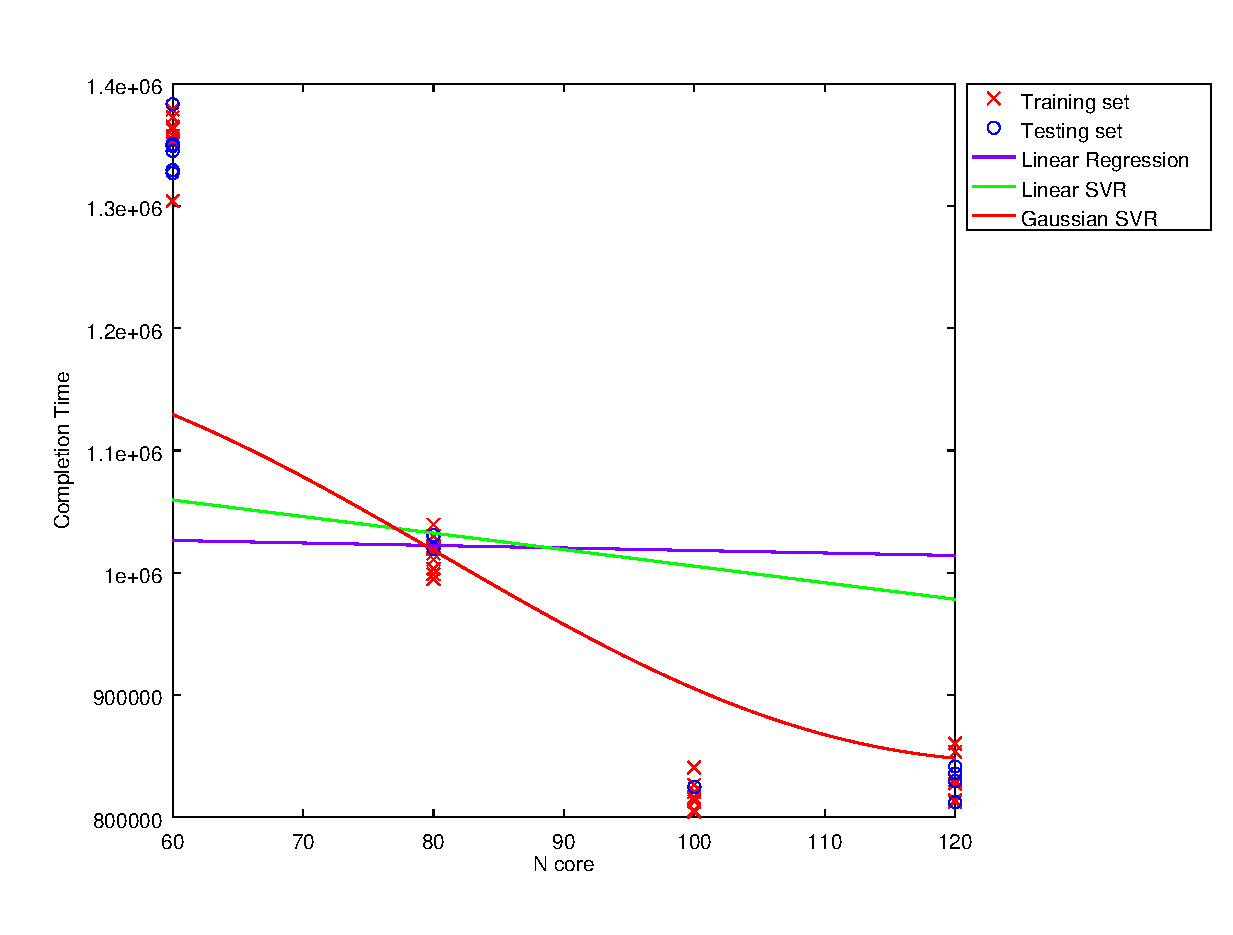
\includegraphics[width=\textwidth]{output/R3_1000_LINEAR_NCORE/plot_R3_1000_bestmodels.eps}
\caption{Completion time vs ncores for query R3 with datasize 1000}
\label{fig:all_linear_R3_1000}
\end {figure}

\newpage
\subsection{Query R4}
\subsubsection{Query R4 -- Datasize 250}
\begin{table}[H]
	\centering
	\begin{adjustbox}{center}
		\begin{tabular}{c | c M{1.2cm} M{2.5cm} M{2.5cm} M{1.8cm}}
			Model & RMSE & R\textsuperscript{2} & Mean absolute error & Mean relative error & Mean difference \tabularnewline
			\hline
			Linear regression & 0.0978 & 0.9896 & 145623 & 0.1950 & 0.0402 \\
			Linear SVR & 0.0868 & 0.9921 & 145413 & 0.1698 & 0.0139 \\
			Polynomial SVR (2) & 0.9021 & 0.3769 & 176046 & 4.1390 & 0.0449 \\
			Polynomial SVR (3) & 0.4383 & 0.8109 & 158227 & 1.5337 & -0.0472 \\
			Polynomial SVR (4) & 0.7075 & 0.4704 & 166908 & 5.1402 & -0.1096 \\
			Polynomial SVR (6) & 0.7548 & 0.4287 & 169159 & 6.1307 & -0.2045 \\
			Gaussian SVR & 0.1831 & 0.9780 & 148802 & 0.3789 & -0.0181 \\
		\end{tabular}
	\end{adjustbox}
	\\
	\caption{Results for R4-250}
	\label{fig:all_linear_R4_250}
\end{table}

\begin {figure}[hbtp]
\centering
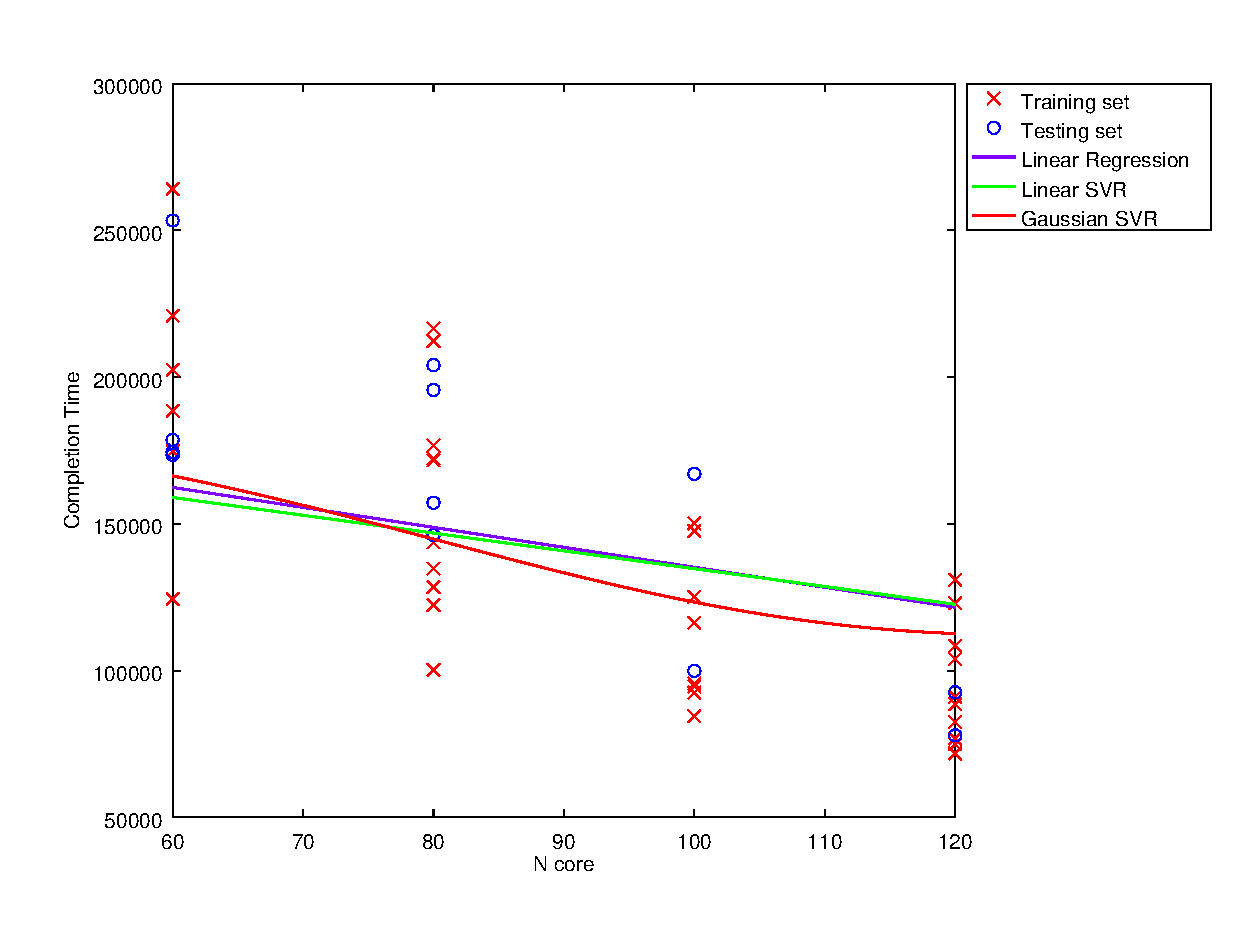
\includegraphics[width=\textwidth]{output/R4_250_LINEAR_NCORE/plot_R4_250_bestmodels.eps}
\caption{Completion time vs ncores for query R4 with datasize 250}
\label{fig:all_linear_R4_250}
\end {figure}

\newpage
\subsubsection{Query R4 -- Datasize 500}
\begin{table}[H]
	\centering
	\begin{adjustbox}{center}
		\begin{tabular}{c | c M{1.2cm} M{2.5cm} M{2.5cm} M{1.8cm}}
			Model & RMSE & R\textsuperscript{2} & Mean absolute error & Mean relative error & Mean difference \tabularnewline
			\hline
			Linear regression & 0.1108 & 0.9886 & 462365 & 0.0884 & -0.0602 \\
			Linear SVR & 0.1631 & 0.9825 & 470614 & 0.1566 & -0.0834 \\
			Polynomial SVR (2) & 0.7309 & 0.5773 & 544504 & 1.9639 & 0.2660 \\
			Polynomial SVR (3) & 0.3500 & 0.9056 & 485019 & 0.2526 & -0.0776 \\
			Polynomial SVR (4) & 0.6397 & 0.6977 & 523293 & 1.0907 & 0.2907 \\
			Polynomial SVR (6) & 0.5599 & 0.7797 & 515591 & 4.6778 & 0.2777 \\
			Gaussian SVR & 0.1726 & 0.9821 & 470779 & 0.4858 & 0.0942 \\
		\end{tabular}
	\end{adjustbox}
	\\
	\caption{Results for R4-500}
	\label{fig:all_linear_R4_500}
\end{table}

\begin {figure}[hbtp]
\centering
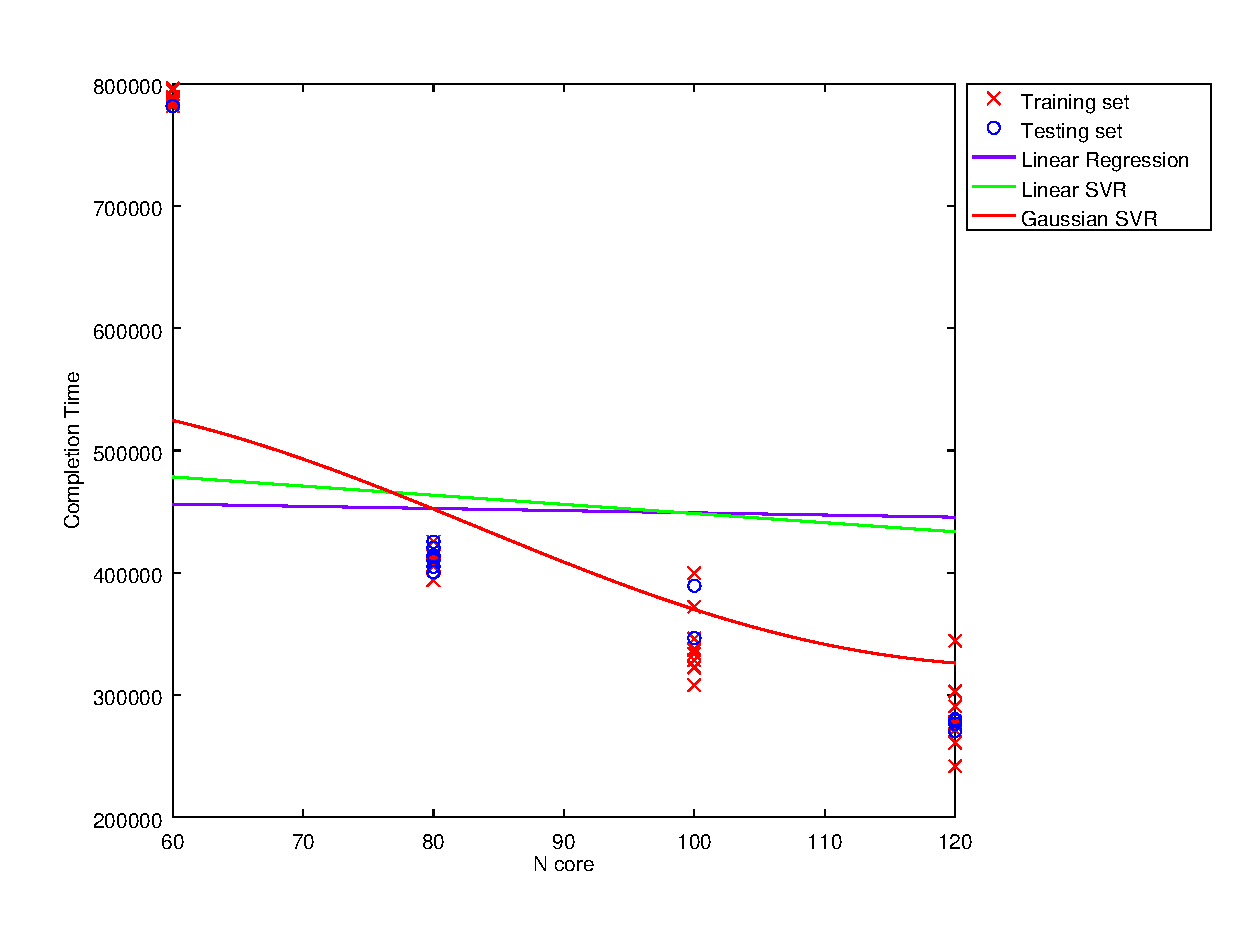
\includegraphics[width=\textwidth]{output/R4_500_LINEAR_NCORE/plot_R4_500_bestmodels.eps}
\caption{Completion time vs ncores for query R4 with datasize 500}
\label{fig:all_linear_R4_500}
\end {figure}

\newpage
\subsubsection{Query R4 -- Datasize 750}
\begin{table}[H]
	\centering
	\begin{adjustbox}{center}
		\begin{tabular}{c | c M{1.2cm} M{2.5cm} M{2.5cm} M{1.8cm}}
			Model & RMSE & R\textsuperscript{2} & Mean absolute error & Mean relative error & Mean difference \tabularnewline
			\hline
			Linear regression & 0.0255 & 0.9992 & 609804 & 0.0775 & -0.0103 \\
			Linear SVR & 0.0855 & 0.9918 & 617776 & 0.2040 & -0.0011 \\
			Polynomial SVR (2) & 0.6525 & 0.5467 & 687086 & 1.5598 & 0.0196 \\
			Polynomial SVR (3) & 0.2783 & 0.9260 & 633333 & 5.1457 & 0.1062 \\
			Polynomial SVR (4) & 0.7808 & 0.5636 & 693469 & 18.2217 & 0.0076 \\
			Polynomial SVR (6) & 0.8117 & 0.6201 & 696905 & 4.7255 & 0.0330 \\
			Gaussian SVR & 0.2473 & 0.9547 & 631812 & 0.5078 & 0.0401 \\
		\end{tabular}
	\end{adjustbox}
	\\
	\caption{Results for R4-750}
	\label{fig:all_linear_R4_750}
\end{table}

\begin {figure}[hbtp]
\centering
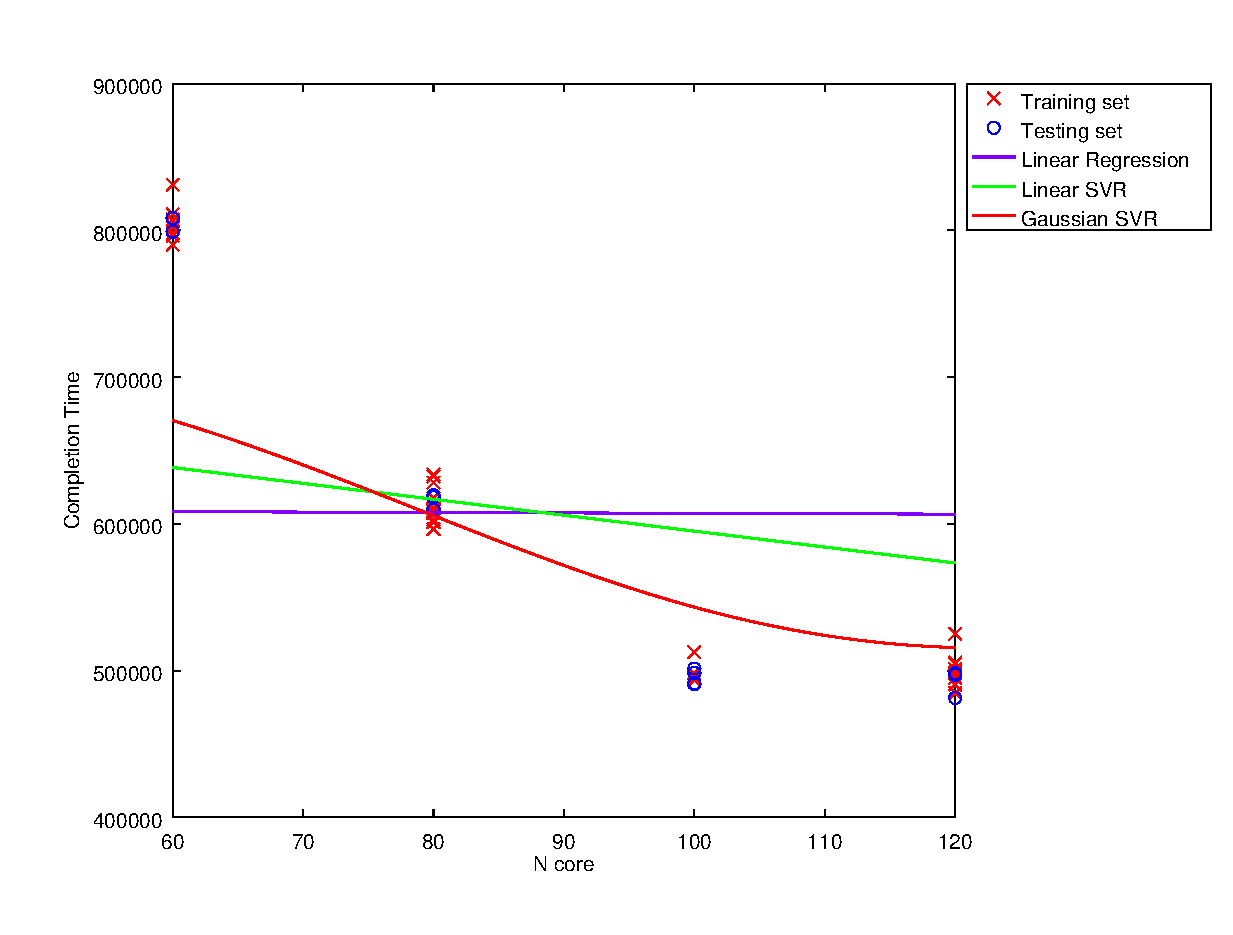
\includegraphics[width=\textwidth]{output/R4_750_LINEAR_NCORE/plot_R4_750_bestmodels.eps}
\caption{Completion time vs ncores for query R4 with datasize 750}
\label{fig:all_linear_R4_750}
\end {figure}

\newpage
\subsubsection{Query R4 -- Datasize 1000}
\begin{table}[H]
	\centering
	\begin{adjustbox}{center}
		\begin{tabular}{c | c M{1.2cm} M{2.5cm} M{2.5cm} M{1.8cm}}
			Model & RMSE & R\textsuperscript{2} & Mean absolute error & Mean relative error & Mean difference \tabularnewline
			\hline
			Linear regression & 0.1381 & 0.9805 & 1804008 & 0.4600 & -0.0308 \\
			Linear SVR & 0.1499 & 0.9780 & 1813721 & 0.3504 & -0.0294 \\
			Polynomial SVR (2) & 0.6424 & 0.6139 & 2199589 & 4.4349 & 0.1704 \\
			Polynomial SVR (3) & 0.9305 & 0.6699 & 2185478 & 7.9108 & 0.2080 \\
			Polynomial SVR (4) & 1.6562 & 0.5290 & 2441940 & 7.0451 & 0.3639 \\
			Polynomial SVR (6) & 2.7937 & 0.4828 & 2740708 & 6.7236 & 0.6345 \\
			Gaussian SVR & 0.3607 & 0.8849 & 1876365 & 0.3316 & -0.1021 \\
		\end{tabular}
	\end{adjustbox}
	\\
	\caption{Results for R4-1000}
	\label{fig:all_linear_R4_1000}
\end{table}

\begin {figure}[hbtp]
\centering
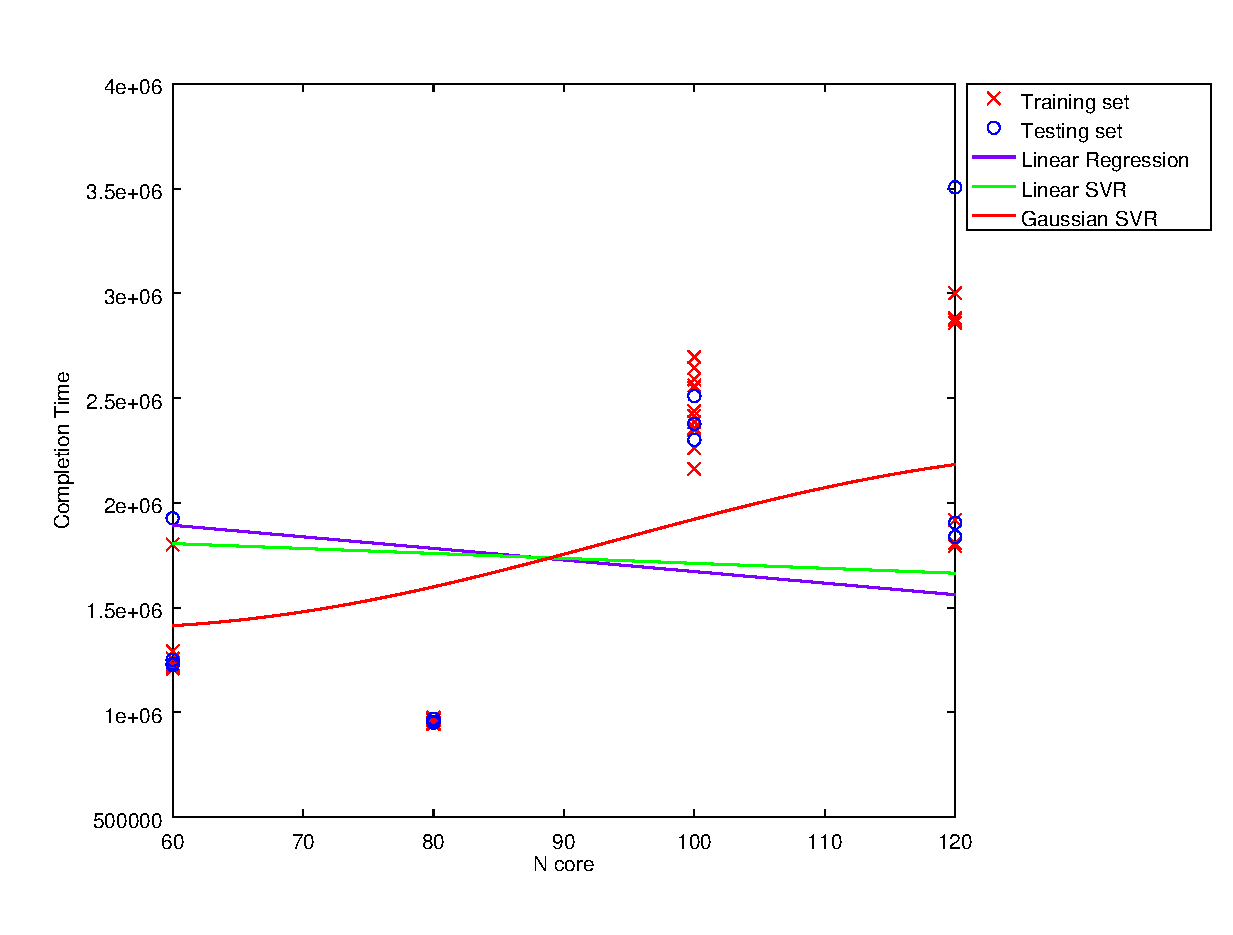
\includegraphics[width=\textwidth]{output/R4_1000_LINEAR_NCORE/plot_R4_1000_bestmodels.eps}
\caption{Completion time vs ncores for query R4 with datasize 1000}
\label{fig:all_linear_R4_1000}
\end {figure}

\newpage
\subsection{Query R5}
\subsubsection{Query R5 -- Datasize 250}

\begin{table}[H]
	\centering
	\begin{adjustbox}{center}
		\begin{tabular}{c | c M{1.2cm} M{2.5cm} M{2.5cm} M{1.8cm}}
			Model & RMSE & R\textsuperscript{2} & Mean absolute error & Mean relative error & Mean difference \tabularnewline
			\hline
			Linear regression & 0.7965 & 0.4265 &  25688 & 1.2827 & 0.0152 \\
			Linear SVR & 0.8069 & 0.4848 &  25686 & 2.0375 & 0.0249 \\
			Polynomial SVR (2) & 1.0778 & 0.0441 &  25968 & 3.1023 & 0.0848 \\
			Polynomial SVR (3) & 1.1435 & 0.2020 &  26070 & 3.6670 & 0.4487 \\
			Polynomial SVR (4) & 1.0392 & 0.0249 &  25845 & 38.4714 & 0.0357 \\
			Polynomial SVR (6) & 1.1437 & 0.0000 &  26070 & 3.6631 & 0.4490 \\
			Gaussian SVR & 0.7553 & 0.4996 &  25722 & 0.9501 & -0.1234 \\
		\end{tabular}
	\end{adjustbox}
	\\
	\caption{Results for R5-250}
	\label{fig:all_linear_R5_250}
\end{table}

\begin {figure}[hbtp]
\centering
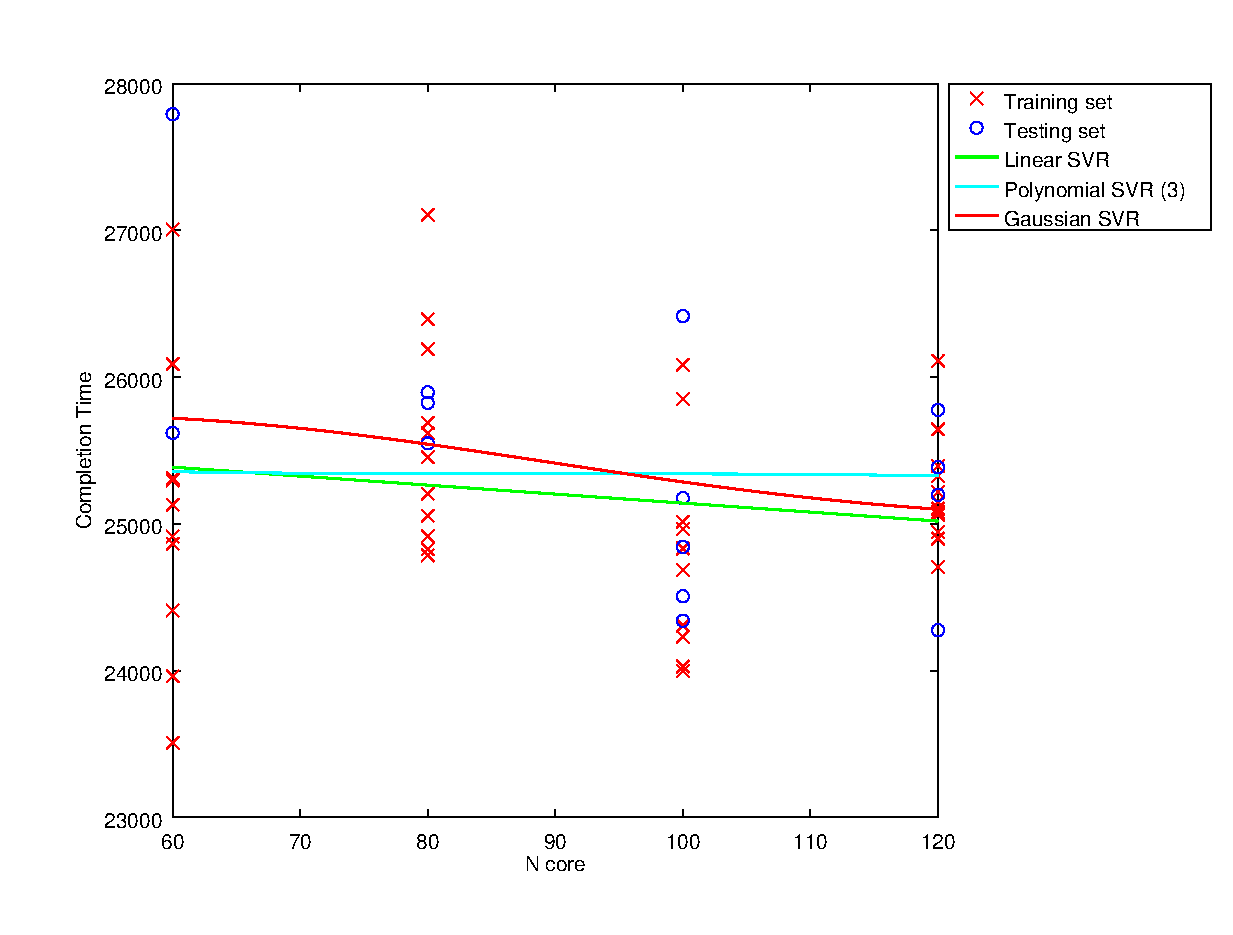
\includegraphics[width=\textwidth]{output/R5_250_LINEAR_NCORE/plot_R5_250_bestmodels.eps}
\caption{Completion time vs ncores for query R5 with datasize 250}
\label{fig:all_linear_R5_250}
\end {figure}

\newpage
\subsubsection{Query R5 -- Datasize 500}
\begin{table}[H]
	\centering
	\begin{adjustbox}{center}
		\begin{tabular}{c | c M{1.2cm} M{2.5cm} M{2.5cm} M{1.8cm}}
			Model & RMSE & R\textsuperscript{2} & Mean absolute error & Mean relative error & Mean difference \tabularnewline
			\hline
			Linear regression & 0.2335 & 0.9462 &  23773 & 0.2129 & -0.0094 \\
			Linear SVR & 0.1635 & 0.9759 &  23707 & 0.1380 & -0.0400 \\
			Polynomial SVR (2) & 0.7958 & 0.6893 &  24451 & 11.3752 & 0.2039 \\
			Polynomial SVR (3) & 0.6675 & 0.6642 &  24047 & 0.4970 & -0.1076 \\
			Polynomial SVR (4) & 1.0322 & 0.1199 &  24583 & 5.8286 & 0.3847 \\
			Polynomial SVR (6) & 2.7907 & 0.0083 &  25512 & 12.6170 & 1.0738 \\
			Gaussian SVR & 0.2252 & 0.9546 &  23774 & 0.2359 & -0.0122 \\
		\end{tabular}
	\end{adjustbox}
	\\
	\caption{Results for R5-500}
	\label{fig:all_linear_R5_500}
\end{table}

\begin {figure}[hbtp]
\centering
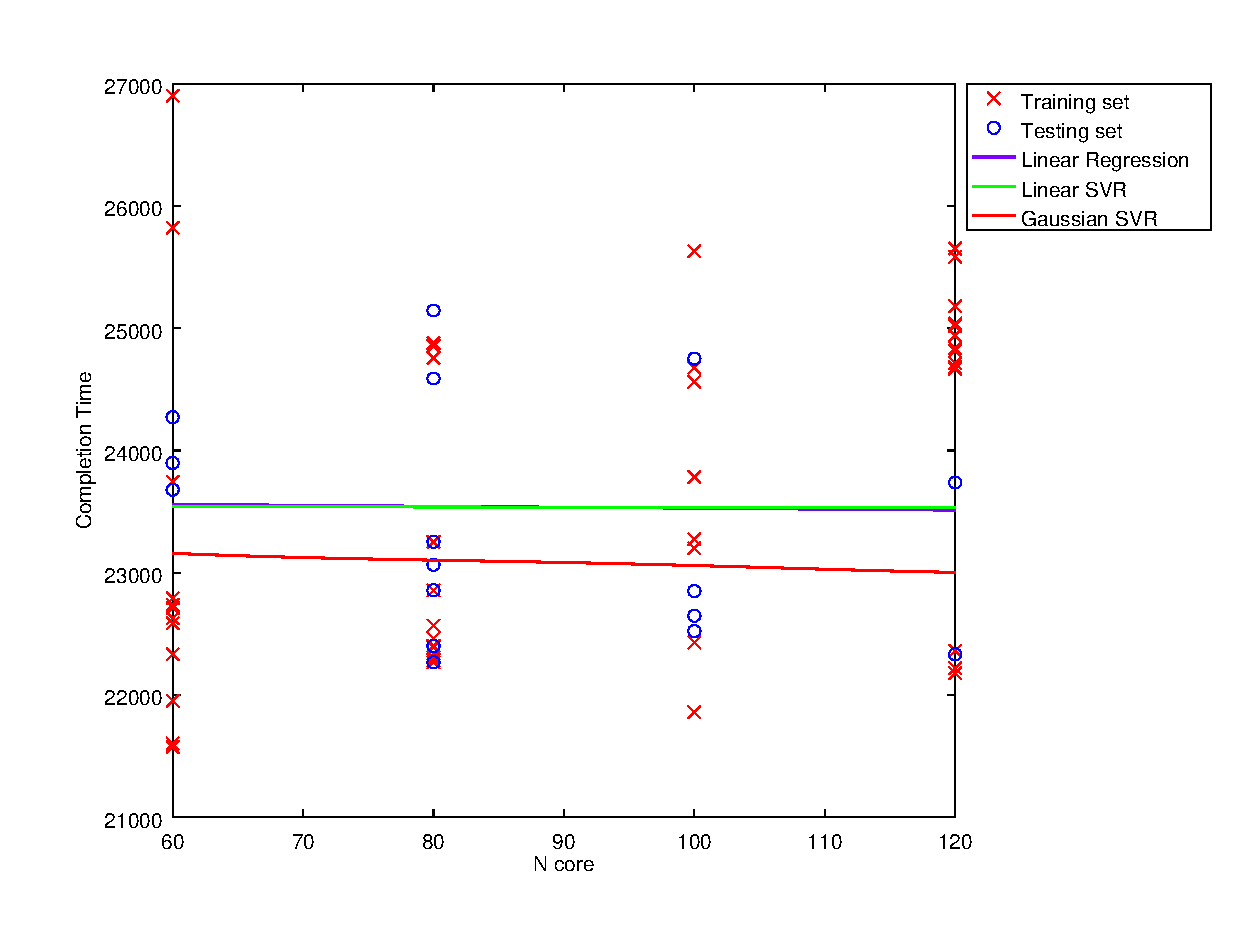
\includegraphics[width=\textwidth]{output/R5_500_LINEAR_NCORE/plot_R5_500_bestmodels.eps}
\caption{Completion time vs ncores for query R5 with datasize 500}
\label{fig:all_linear_R5_500}
\end {figure}

\newpage
\subsubsection{Query R5 -- Datasize 750}
\begin{table}[H]
	\centering
	\begin{adjustbox}{center}
		\begin{tabular}{c | c M{1.2cm} M{2.5cm} M{2.5cm} M{1.8cm}}
			Model & RMSE & R\textsuperscript{2} & Mean absolute error & Mean relative error & Mean difference \tabularnewline
			\hline
			Linear regression & 1.2490 & -0.6264 &  24815 & 1.1406 & -0.3032 \\
			Linear SVR & 1.1195 & 0.0143 &  24794 & 2.7234 & -0.2486 \\
			Polynomial SVR (2) & 1.0444 & 0.0002 &  25027 & 5.3705 & -0.3557 \\
			Polynomial SVR (3) & 1.2104 & 0.0337 &  24862 & 1.5255 & -0.3448 \\
			Polynomial SVR (4) & 1.0613 & 0.0307 &  25044 & 17.5373 & -0.3810 \\
			Polynomial SVR (6) & 1.0719 & 0.0710 &  25053 & 9.2745 & -0.4046 \\
			Gaussian SVR & 0.9913 & 0.2058 &  24635 & 1.2416 & -0.3754 \\
		\end{tabular}
	\end{adjustbox}
	\\
	\caption{Results for R5-750}
	\label{fig:all_linear_R5_750}
\end{table}

\begin {figure}[hbtp]
\centering
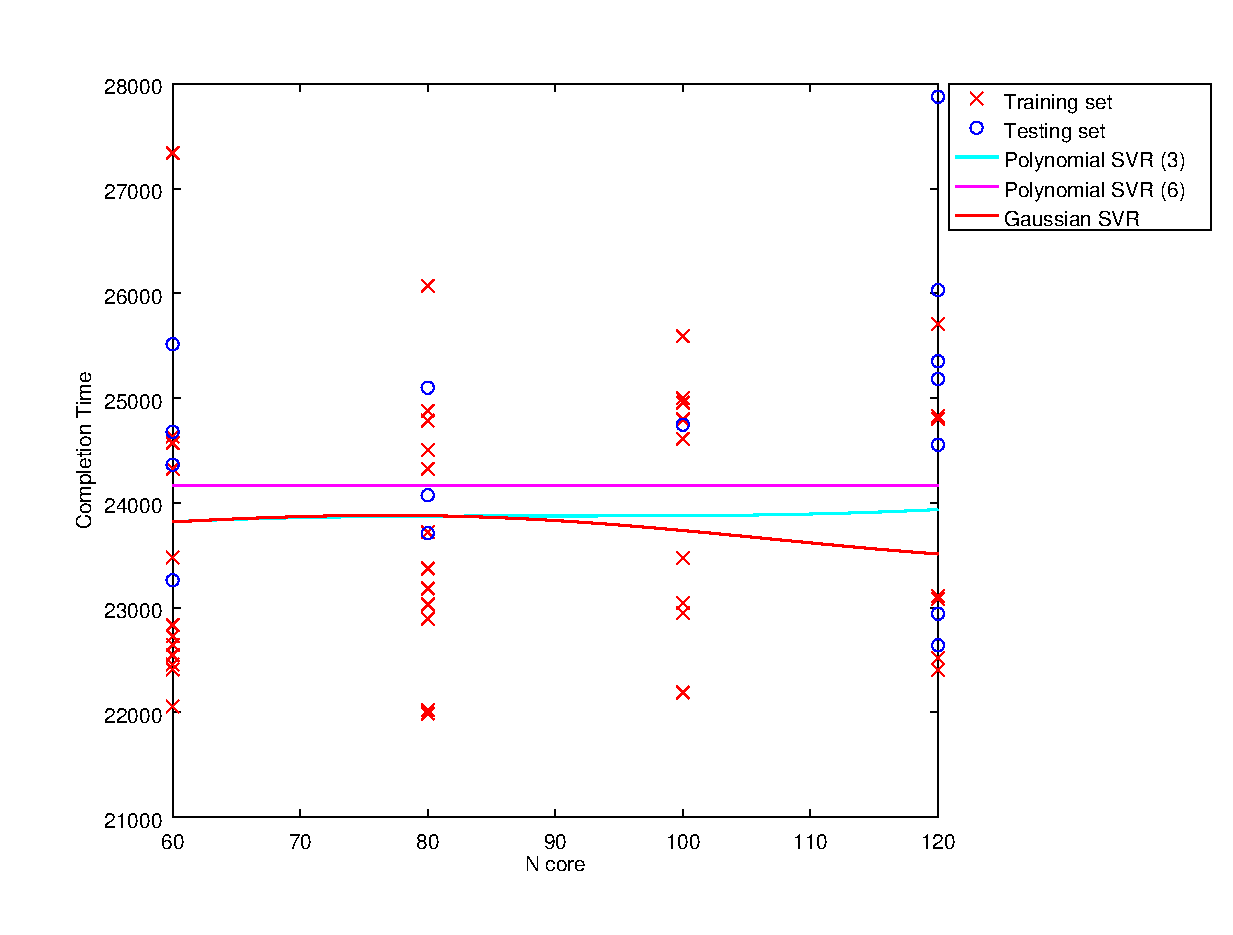
\includegraphics[width=\textwidth]{output/R5_750_LINEAR_NCORE/plot_R5_750_bestmodels.eps}
\caption{Completion time vs ncores for query R5 with datasize 750}
\label{fig:all_linear_R5_750}
\end {figure}

\newpage
\subsubsection{Query R5 -- Datasize 1000}
\begin{table}[H]
	\centering
	\begin{adjustbox}{center}
		\begin{tabular}{c | c M{1.2cm} M{2.5cm} M{2.5cm} M{1.8cm}}
			Model & RMSE & R\textsuperscript{2} & Mean absolute error & Mean relative error & Mean difference \tabularnewline
			\hline
			Linear regression & 0.7715 & 0.1365 &  40268 & 4.8095 & 0.1134 \\
			Linear SVR & 0.4840 & 0.6667 &  39598 & 1.5763 & -0.0352 \\
			Polynomial SVR (2) & 0.5299 & 0.8033 &  39459 & 0.6997 & 0.1937 \\
			Polynomial SVR (3) & 0.4527 & 0.7609 &  39368 & 0.6924 & 0.0637 \\
			Polynomial SVR (4) & 2.1454 & 0.6726 &  41543 & 0.9574 & 0.7941 \\
			Polynomial SVR (6) & 8.5650 & 0.5560 &  49272 & 1.8561 & 2.9480 \\
			Gaussian SVR & 0.3378 & 0.8434 &  39075 & 0.6641 & 0.0550 \\
		\end{tabular}
	\end{adjustbox}
	\\
	\caption{Results for R5-1000}
	\label{fig:all_linear_R5_1000}
\end{table}

\begin {figure}[hbtp]
\centering
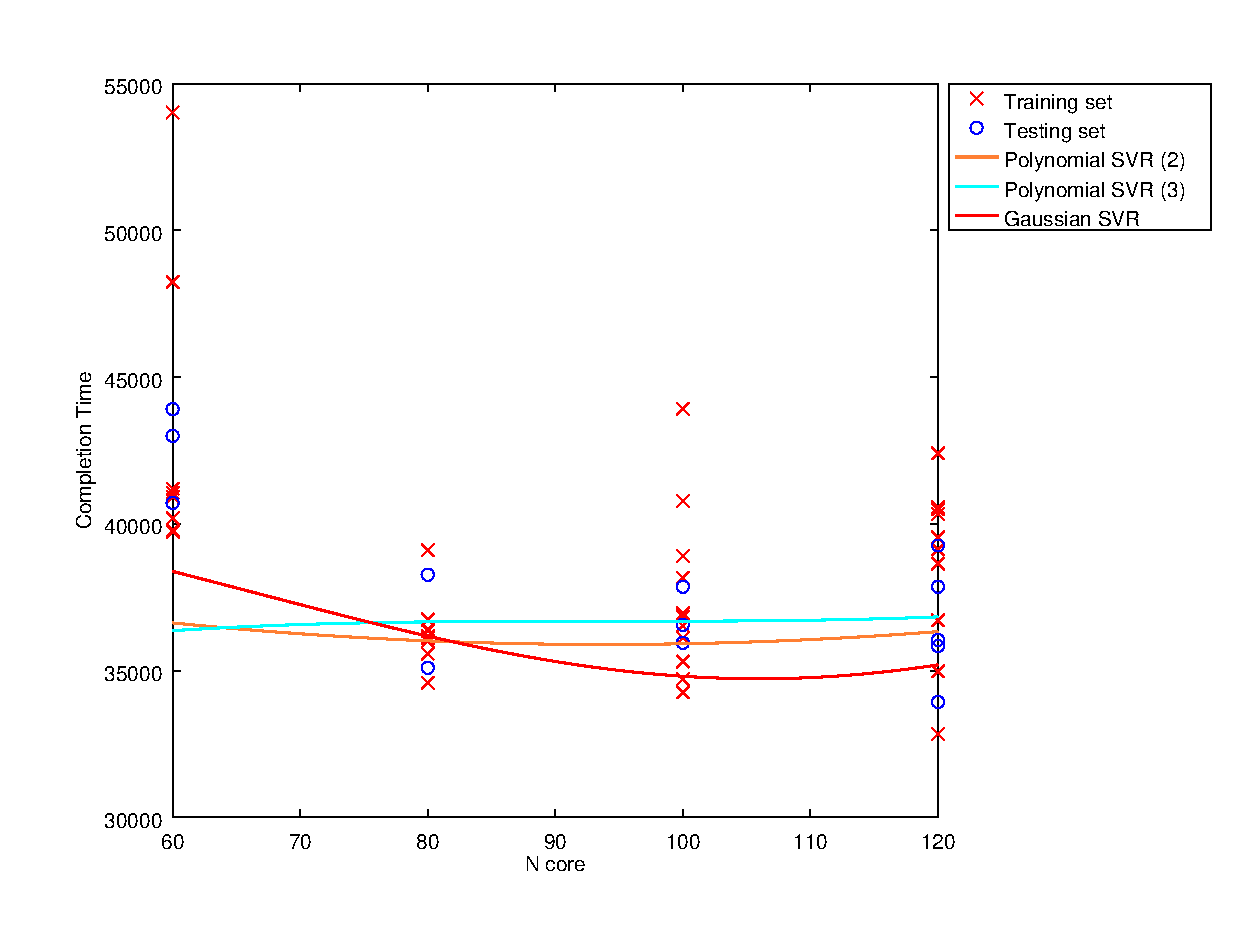
\includegraphics[width=\textwidth]{output/R5_1000_LINEAR_NCORE/plot_R5_1000_bestmodels.eps}
\caption{Completion time vs ncores for query R5 with datasize 1000}
\label{fig:all_linear_R5_1000}
\end {figure}

%--------------------------------------------

\newpage
\section{Fixed Datasize, Only $ncores$}
\subsection{Query R1}
\subsubsection{Query R1 -- Datasize 250}
\begin{table}[H]
	\centering
	\begin{adjustbox}{center}
		\begin{tabular}{c | c M{1.2cm} M{2.5cm} M{2.5cm} M{1.8cm}}
			Model & RMSE & R\textsuperscript{2} & Mean absolute error & Mean relative error & Mean difference \tabularnewline
			\hline
			Linear regression & 1.2075 & 0.3647 &  68861 & 1.6258 & -0.3635 \\
			Linear SVR & 1.2849 & 0.4436 &  68595 & 6.2353 & -0.4838 \\
			Polynomial SVR (2) & 1.5934 & 0.0830 &  80355 & 8.0774 & -0.2627 \\
			Polynomial SVR (3) & 1.3520 & 0.3512 &  70155 & 2.7404 & -0.5287 \\
			Polynomial SVR (4) & 1.5463 & 0.0938 &  79717 & 21.6531 & -0.3012 \\
			Polynomial SVR (6) & 1.5344 & 0.1080 &  79664 & 84.7876 & -0.2897 \\
			Gaussian SVR & 1.2809 & 0.4200 &  69434 & 8.6924 & -0.4253 \\
		\end{tabular}
	\end{adjustbox}
	\\
	\caption{Results for R1-250}
	\label{fig:coreonly_linear_R1_250}
\end{table}

\begin {figure}[hbtp]
\centering
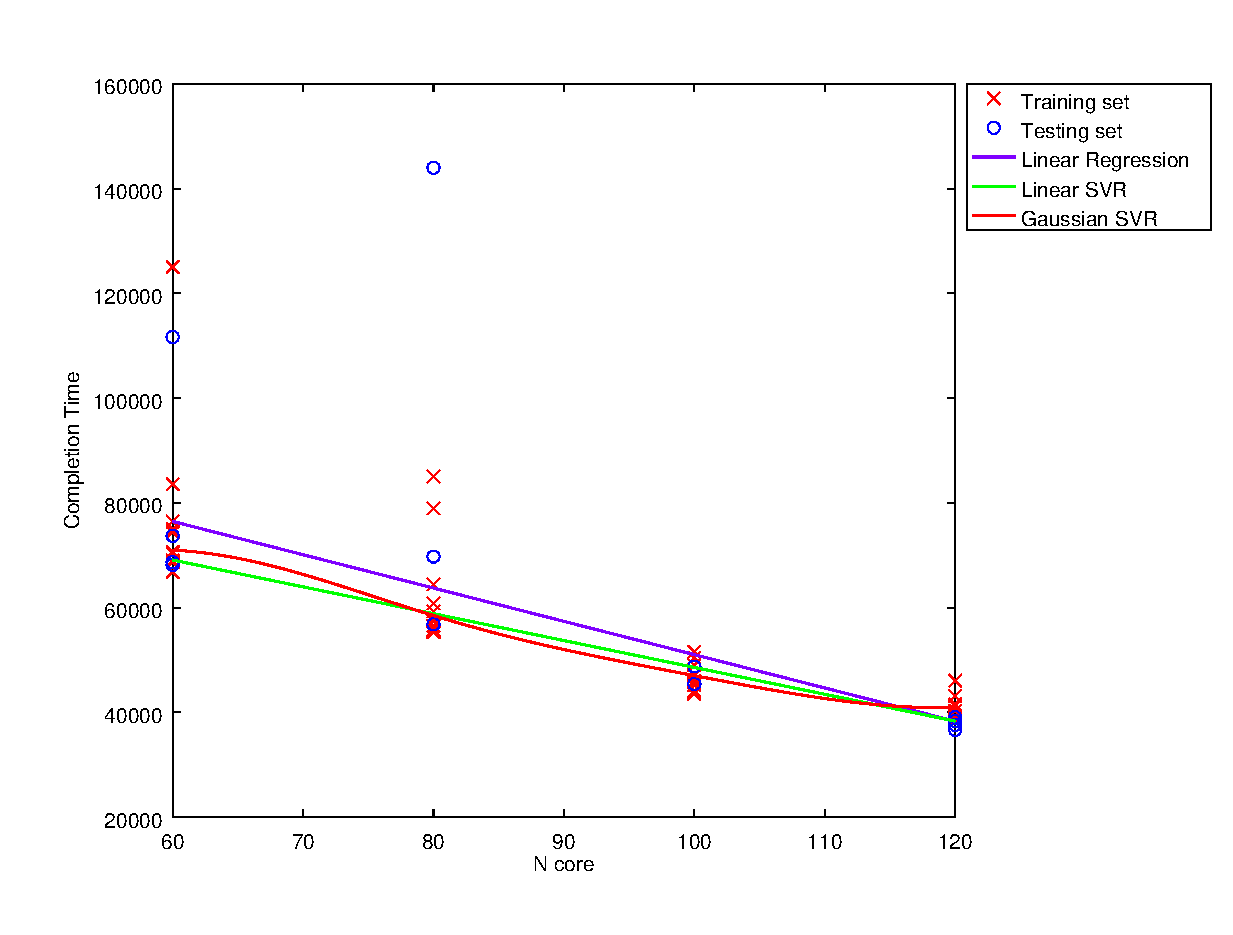
\includegraphics[width=\textwidth]{output/R1_250_ONLY_1_LINEAR_NCORE/plot_R1_250_bestmodels.eps}
\caption{Completion time vs ncores for query R1 with datasize 250}
\label{fig:coreonly_linear_R1_250}
\end {figure}

\newpage
\subsubsection{Query R1 -- Datasize 500}
\begin{table}[H]
	\centering
	\begin{adjustbox}{center}
		\begin{tabular}{c | c M{1.2cm} M{2.5cm} M{2.5cm} M{1.8cm}}
			Model & RMSE & R\textsuperscript{2} & Mean absolute error & Mean relative error & Mean difference \tabularnewline
			\hline
			Linear regression & 0.7251 & 0.4405 & 210667 & 1.2210 & 0.0864 \\
			Linear SVR & 0.7201 & 0.4486 & 209619 & 1.2525 & 0.0171 \\
			Polynomial SVR (2) & 0.8432 & 0.2950 & 205970 & 1.2352 & -0.1621 \\
			Polynomial SVR (3) & 0.5801 & 0.6689 & 197539 & 28.1452 & 0.0446 \\
			Polynomial SVR (4) & 0.8077 & 0.3221 & 206099 & 1.2816 & -0.0362 \\
			Polynomial SVR (6) & 0.9428 & 0.3521 & 206106 & 13.9256 & -0.3429 \\
			Gaussian SVR & 0.3223 & 0.8986 & 181637 & 1.0628 & -0.0234 \\
		\end{tabular}
	\end{adjustbox}
	\\
	\caption{Results for R1-500}
	\label{fig:coreonly_linear_R1_500}
\end{table}

\begin {figure}[hbtp]
\centering
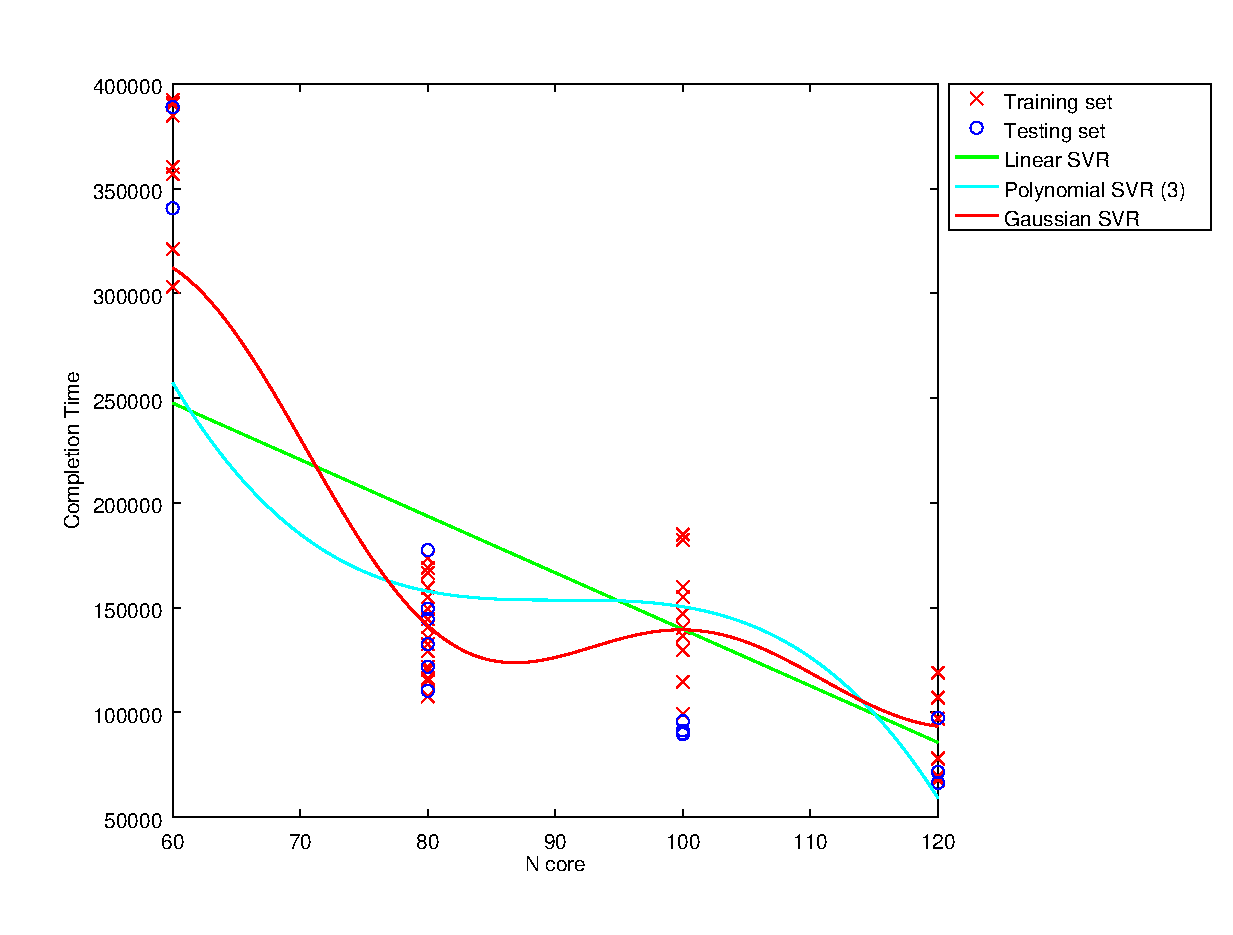
\includegraphics[width=\textwidth]{output/R1_500_ONLY_1_LINEAR_NCORE/plot_R1_500_bestmodels.eps}
\caption{Completion time vs ncores for query R1 with datasize 500}
\label{fig:coreonly_linear_R1_500}
\end {figure}

\newpage
\subsubsection{Query R1 -- Datasize 750}
\begin{table}[H]
	\centering
	\begin{adjustbox}{center}
		\begin{tabular}{c | c M{1.2cm} M{2.5cm} M{2.5cm} M{1.8cm}}
			Model & RMSE & R\textsuperscript{2} & Mean absolute error & Mean relative error & Mean difference \tabularnewline
			\hline
			Linear regression & 0.6014 & 0.5593 & 300870 & 1.0236 & 0.0563 \\
			Linear SVR & 0.6547 & 0.5657 & 302818 & 1.1093 & 0.2441 \\
			Polynomial SVR (2) & 0.9570 & 0.0585 & 333009 & 3.1518 & 0.3754 \\
			Polynomial SVR (3) & 0.6613 & 0.5999 & 305890 & 2.0590 & 0.3179 \\
			Polynomial SVR (4) & 0.9628 & 0.0628 & 331953 & 1.9881 & 0.3637 \\
			Polynomial SVR (6) & 0.9559 & 0.0677 & 331616 & 1.9227 & 0.3491 \\
			Gaussian SVR & 0.6228 & 0.5829 & 307418 & 1.0560 & 0.1938 \\
		\end{tabular}
	\end{adjustbox}
	\\
	\caption{Results for R1-750}
	\label{fig:coreonly_linear_R1_750}
\end{table}

\begin {figure}[hbtp]
\centering
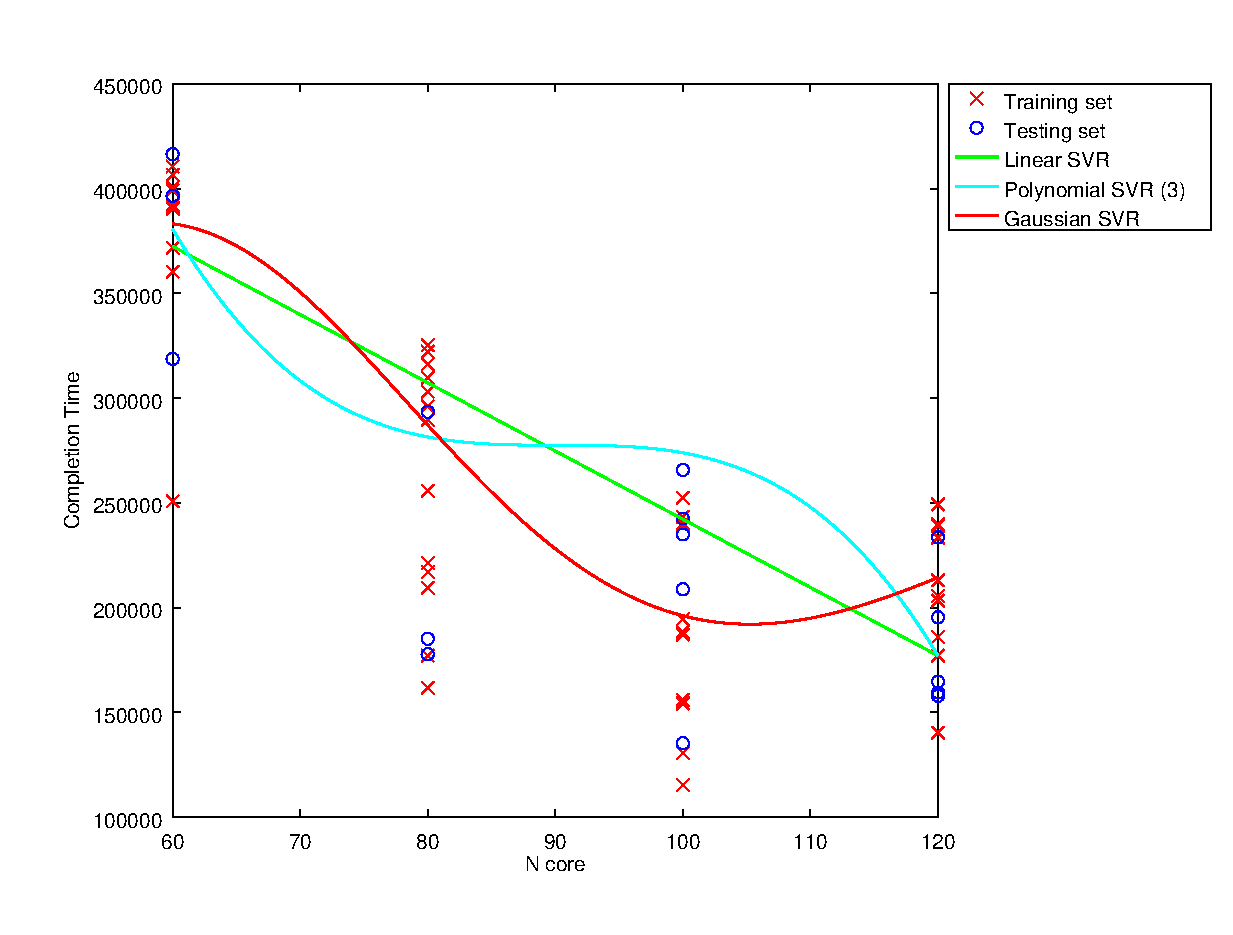
\includegraphics[width=\textwidth]{output/R1_750_ONLY_1_LINEAR_NCORE/plot_R1_750_bestmodels.eps}
\caption{Completion time vs ncores for query R1 with datasize 750}
\label{fig:coreonly_linear_R1_750}
\end {figure}

\newpage
\subsubsection{Query R1 -- Datasize 1000}
\begin{table}[H]
	\centering
	\begin{adjustbox}{center}
		\begin{tabular}{c | c M{1.2cm} M{2.5cm} M{2.5cm} M{1.8cm}}
			Model & RMSE & R\textsuperscript{2} & Mean absolute error & Mean relative error & Mean difference \tabularnewline
			\hline
			Linear regression & 0.6226 & -0.4972 & 473125 & 1.1210 & 0.2951 \\
			Linear SVR & 0.6037 & 0.3347 & 471327 & 1.1101 & 0.2858 \\
			Polynomial SVR (2) & 0.8422 & 0.1330 & 488214 & 2.6598 & 0.4419 \\
			Polynomial SVR (3) & 0.7066 & 0.1527 & 476425 & 3.5287 & 0.3181 \\
			Polynomial SVR (4) & 0.8534 & 0.1296 & 488988 & 2.4699 & 0.4493 \\
			Polynomial SVR (6) & 0.8670 & 0.1289 & 489939 & 2.3029 & 0.4593 \\
			Gaussian SVR & 0.4298 & 0.4559 & 454613 & 1.3229 & 0.2022 \\
		\end{tabular}
	\end{adjustbox}
	\\
	\caption{Results for R1-1000}
	\label{fig:coreonly_linear_R1_1000}
\end{table}

\begin {figure}[hbtp]
\centering
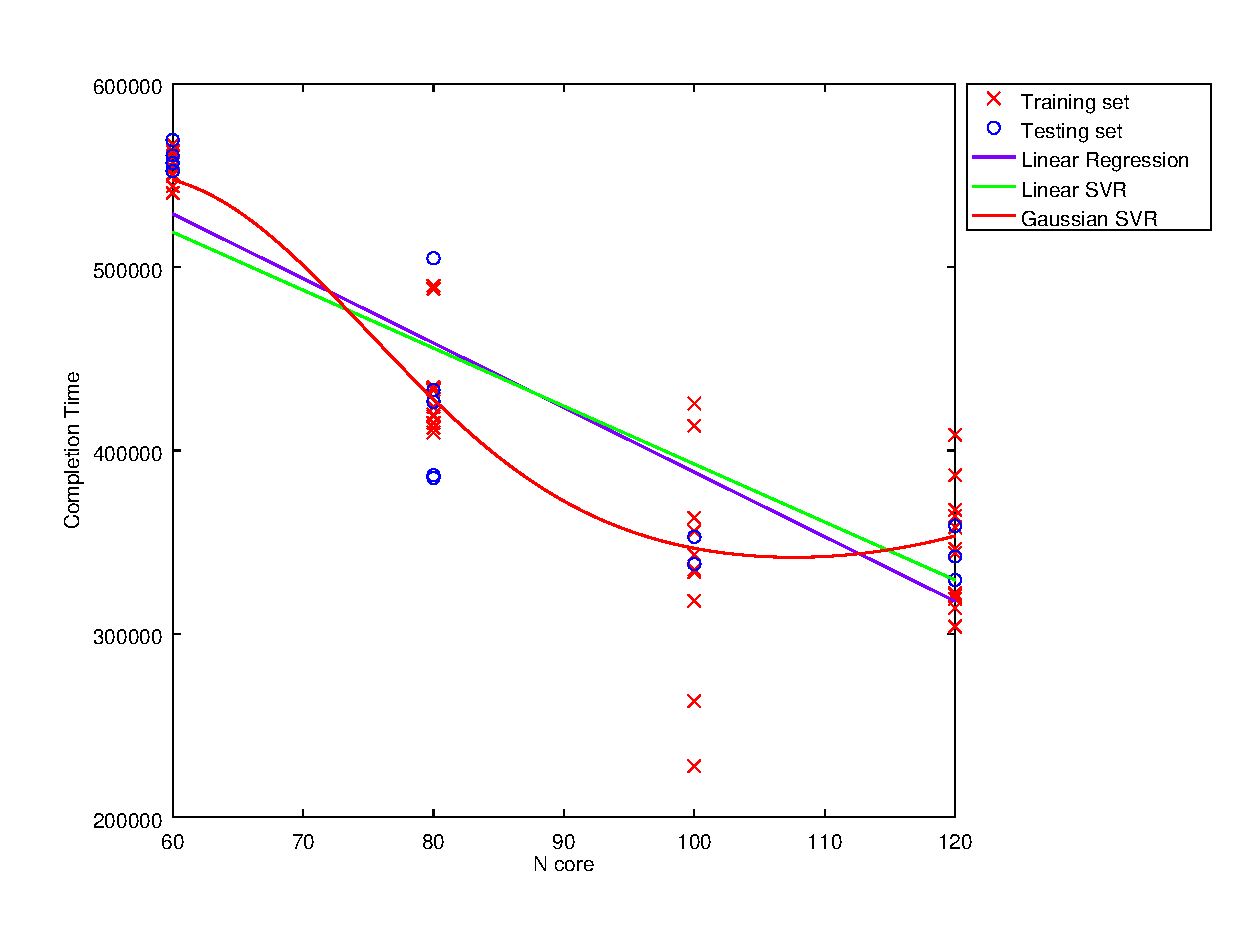
\includegraphics[width=\textwidth]{output/R1_1000_ONLY_1_LINEAR_NCORE/plot_R1_1000_bestmodels.eps}
\caption{Completion time vs ncores for query R1 with datasize 1000}
\label{fig:coreonly_linear_R1_1000}
\end {figure}

\newpage
\subsection{Query R2}
\subsubsection{Query R2 -- Datasize 250}
\begin{table}[H]
	\centering
	\begin{adjustbox}{center}
		\begin{tabular}{c | c M{1.2cm} M{2.5cm} M{2.5cm} M{1.8cm}}
			Model & RMSE & R\textsuperscript{2} & Mean absolute error & Mean relative error & Mean difference \tabularnewline
			\hline
			Linear regression & 1.1128 & -0.1570 &  86628 & 14.4978 & 0.5476 \\
			Linear SVR & 1.0683 & 0.3052 &  86458 & 9.8909 & 0.4767 \\
			Polynomial SVR (2) & 1.2109 & 0.1481 &  86848 & 59.8285 & 0.5888 \\
			Polynomial SVR (3) & 1.0758 & 0.1577 &  86446 & 16.1503 & 0.4411 \\
			Polynomial SVR (4) & 1.2102 & 0.1394 &  86844 & 66.2597 & 0.5879 \\
			Polynomial SVR (6) & 1.2118 & 0.1377 &  86850 & 68.0304 & 0.5896 \\
			Gaussian SVR & 1.1490 & 0.3419 &  86752 & 19.4207 & 0.6036 \\
		\end{tabular}
	\end{adjustbox}
	\\
	\caption{Results for R2-250}
	\label{fig:coreonly_linear_R2_250}
\end{table}

\begin {figure}[hbtp]
\centering
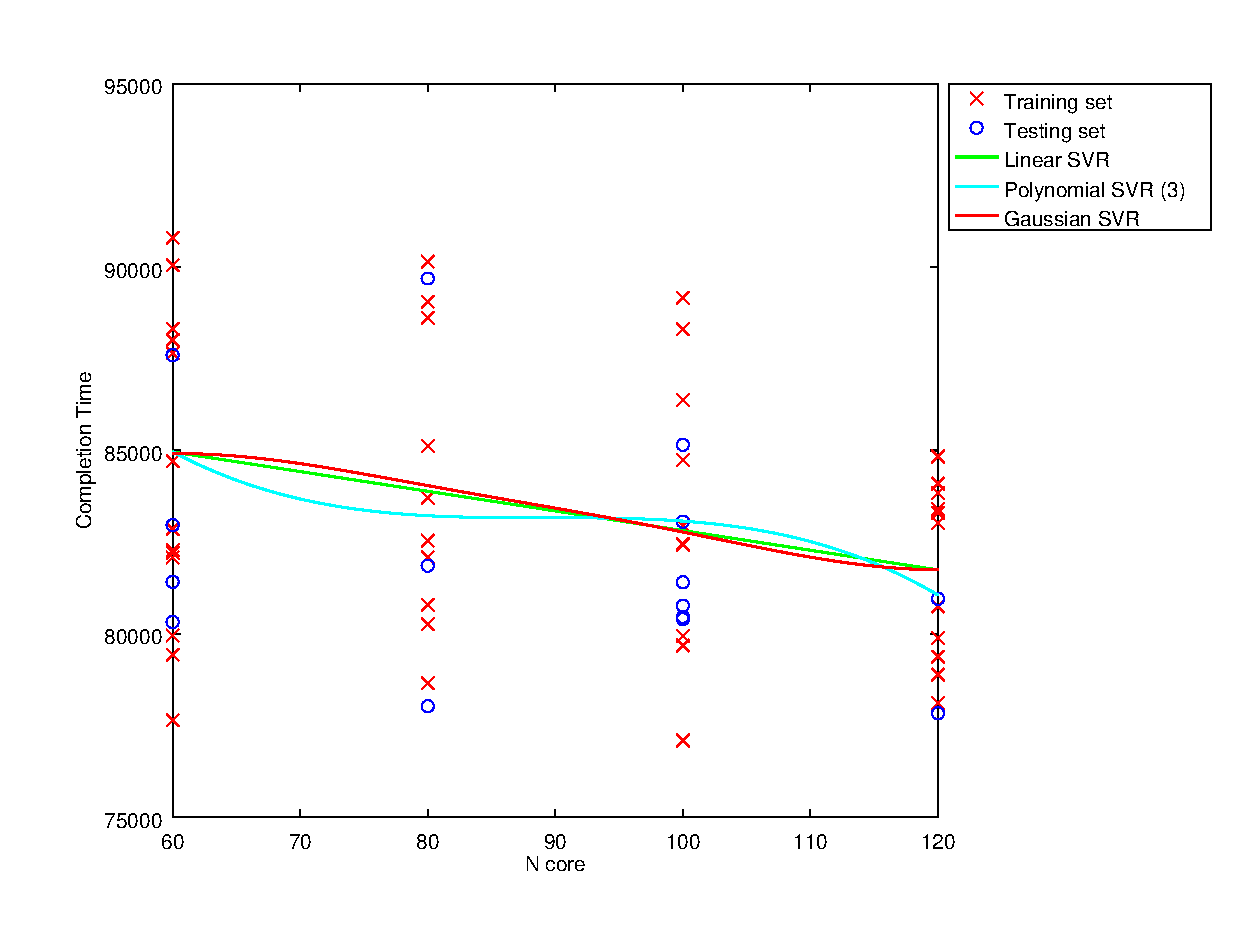
\includegraphics[width=\textwidth]{output/R2_250_ONLY_1_LINEAR_NCORE/plot_R2_250_bestmodels.eps}
\caption{Completion time vs ncores for query R2 with datasize 250}
\label{fig:coreonly_linear_R2_250}
\end {figure}

\newpage
\subsubsection{Query R2 -- Datasize 500}
\begin{table}[H]
	\centering
	\begin{adjustbox}{center}
		\begin{tabular}{c | c M{1.2cm} M{2.5cm} M{2.5cm} M{1.8cm}}
			Model & RMSE & R\textsuperscript{2} & Mean absolute error & Mean relative error & Mean difference \tabularnewline
			\hline
			Linear regression & 0.8543 & -0.0920 &  74969 & 46.7605 & 0.2171 \\
			Linear SVR & 0.9098 & 0.0000 &  75155 & 3.9493 & 0.3992 \\
			Polynomial SVR (2) & 0.8651 & 0.0946 &  74972 & 15.1417 & 0.3568 \\
			Polynomial SVR (3) & 0.9098 & 0.0000 &  75155 & 3.9493 & 0.3992 \\
			Polynomial SVR (4) & 0.8587 & 0.0997 &  74944 & 14.3128 & 0.3458 \\
			Polynomial SVR (6) & 0.9098 & 0.0000 &  75155 & 3.9493 & 0.3992 \\
			Gaussian SVR & 0.9098 & 0.0000 &  75155 & 3.9493 & 0.3992 \\
		\end{tabular}
	\end{adjustbox}
	\\
	\caption{Results for R2-500}
	\label{fig:coreonly_linear_R2_500}
\end{table}

\begin {figure}[hbtp]
\centering
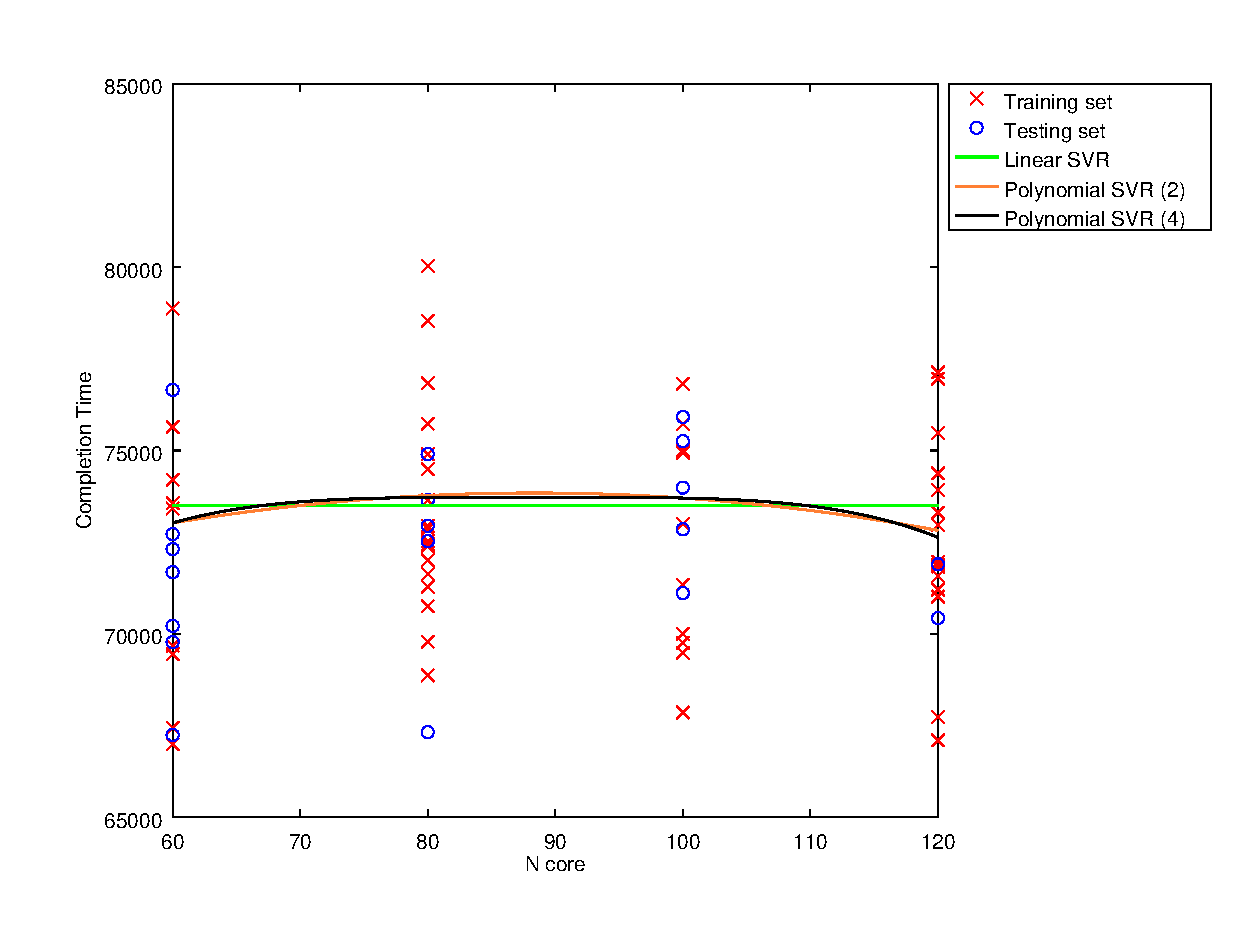
\includegraphics[width=\textwidth]{output/R2_500_ONLY_1_LINEAR_NCORE/plot_R2_500_bestmodels.eps}
\caption{Completion time vs ncores for query R2 with datasize 500}
\label{fig:coreonly_linear_R2_500}
\end {figure}

\newpage
\subsubsection{Query R2 -- Datasize 750}
\begin{table}[H]
	\centering
	\begin{adjustbox}{center}
		\begin{tabular}{c | c M{1.2cm} M{2.5cm} M{2.5cm} M{1.8cm}}
			Model & RMSE & R\textsuperscript{2} & Mean absolute error & Mean relative error & Mean difference \tabularnewline
			\hline
			Linear regression & 1.1529 & -0.8099 &  80556 & 7.5370 & -0.7282 \\
			Linear SVR & 1.1811 & -0.0000 &  80690 & 5.0940 & -0.8127 \\
			Polynomial SVR (2) & 1.1685 & 0.0000 &  80656 & 5.5732 & -0.7944 \\
			Polynomial SVR (3) & 1.1980 & 0.0043 &  80720 & 27.0542 & -0.8330 \\
			Polynomial SVR (4) & 1.1685 & 0.0000 &  80656 & 5.5732 & -0.7944 \\
			Polynomial SVR (6) & 1.1685 & 0.0000 &  80656 & 5.5732 & -0.7944 \\
			Gaussian SVR & 1.1685 & 0.0000 &  80656 & 5.5732 & -0.7944 \\
		\end{tabular}
	\end{adjustbox}
	\\
	\caption{Results for R2-750}
	\label{fig:coreonly_linear_R2_750}
\end{table}

\begin {figure}[hbtp]
\centering
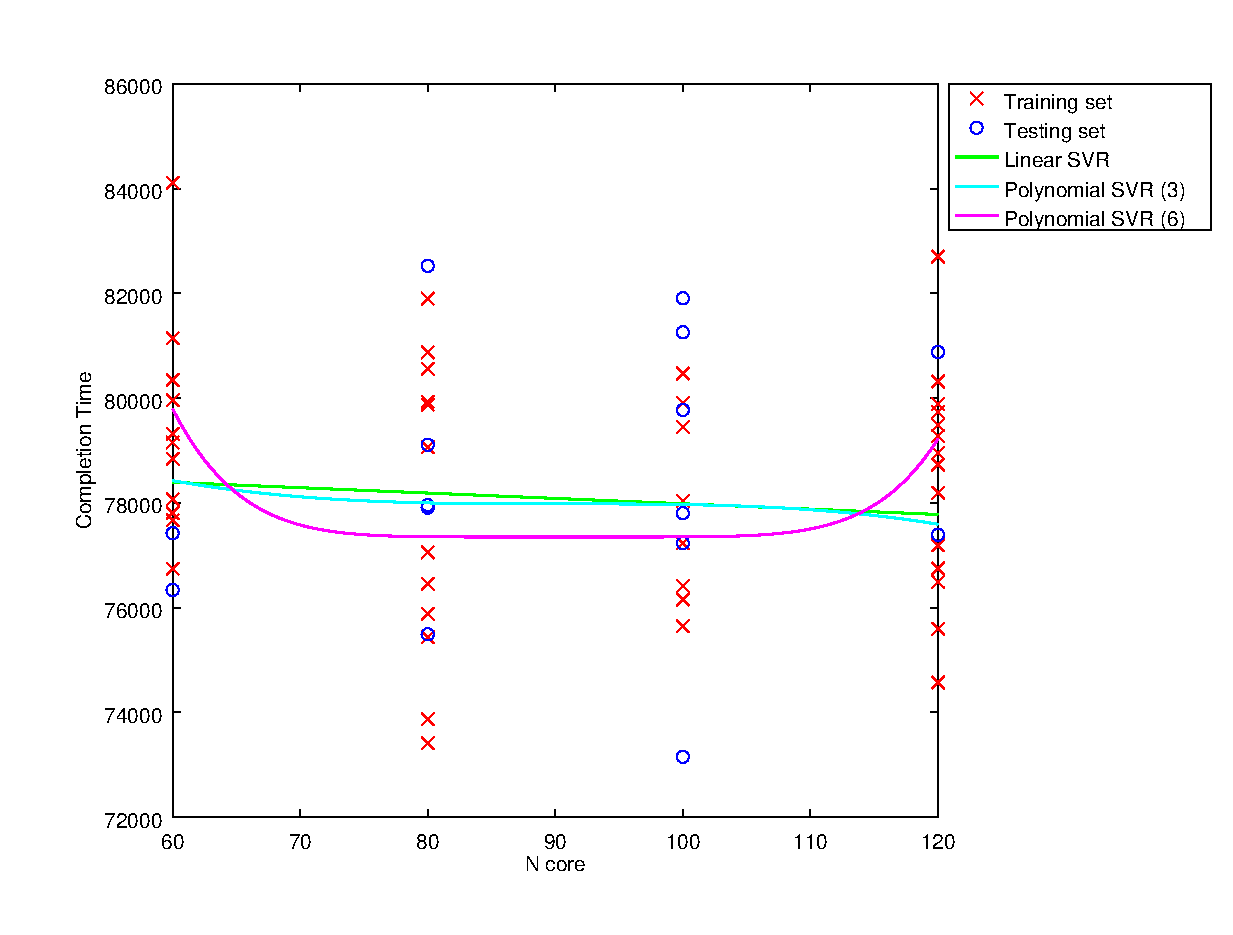
\includegraphics[width=\textwidth]{output/R2_750_ONLY_1_LINEAR_NCORE/plot_R2_750_bestmodels.eps}
\caption{Completion time vs ncores for query R2 with datasize 750}
\label{fig:coreonly_linear_R2_750}
\end {figure}

\newpage
\subsubsection{Query R2 -- Datasize 1000}
\begin{table}[H]
	\centering
	\begin{adjustbox}{center}
		\begin{tabular}{c | c M{1.2cm} M{2.5cm} M{2.5cm} M{1.8cm}}
			Model & RMSE & R\textsuperscript{2} & Mean absolute error & Mean relative error & Mean difference \tabularnewline
			\hline
			Linear regression & 0.4726 & -0.3327 & 1347093 & 0.8336 & 0.1087 \\
			Linear SVR & 0.4949 & 0.5506 & 1359787 & 0.9295 & 0.1621 \\
			Polynomial SVR (2) & 0.9099 & 0.1794 & 1517625 & 1.3713 & 0.3120 \\
			Polynomial SVR (3) & 0.5414 & 0.2285 & 1342325 & 13.9279 & 0.0046 \\
			Polynomial SVR (4) & 0.9474 & 0.1850 & 1528852 & 1.3313 & 0.2292 \\
			Polynomial SVR (6) & 0.9214 & 0.1863 & 1519870 & 1.3624 & 0.2656 \\
			Gaussian SVR & 0.2025 & 0.7958 & 1194571 & 1.1252 & 0.0811 \\
		\end{tabular}
	\end{adjustbox}
	\\
	\caption{Results for R2-1000}
	\label{fig:coreonly_linear_R2_1000}
\end{table}

\begin {figure}[hbtp]
\centering
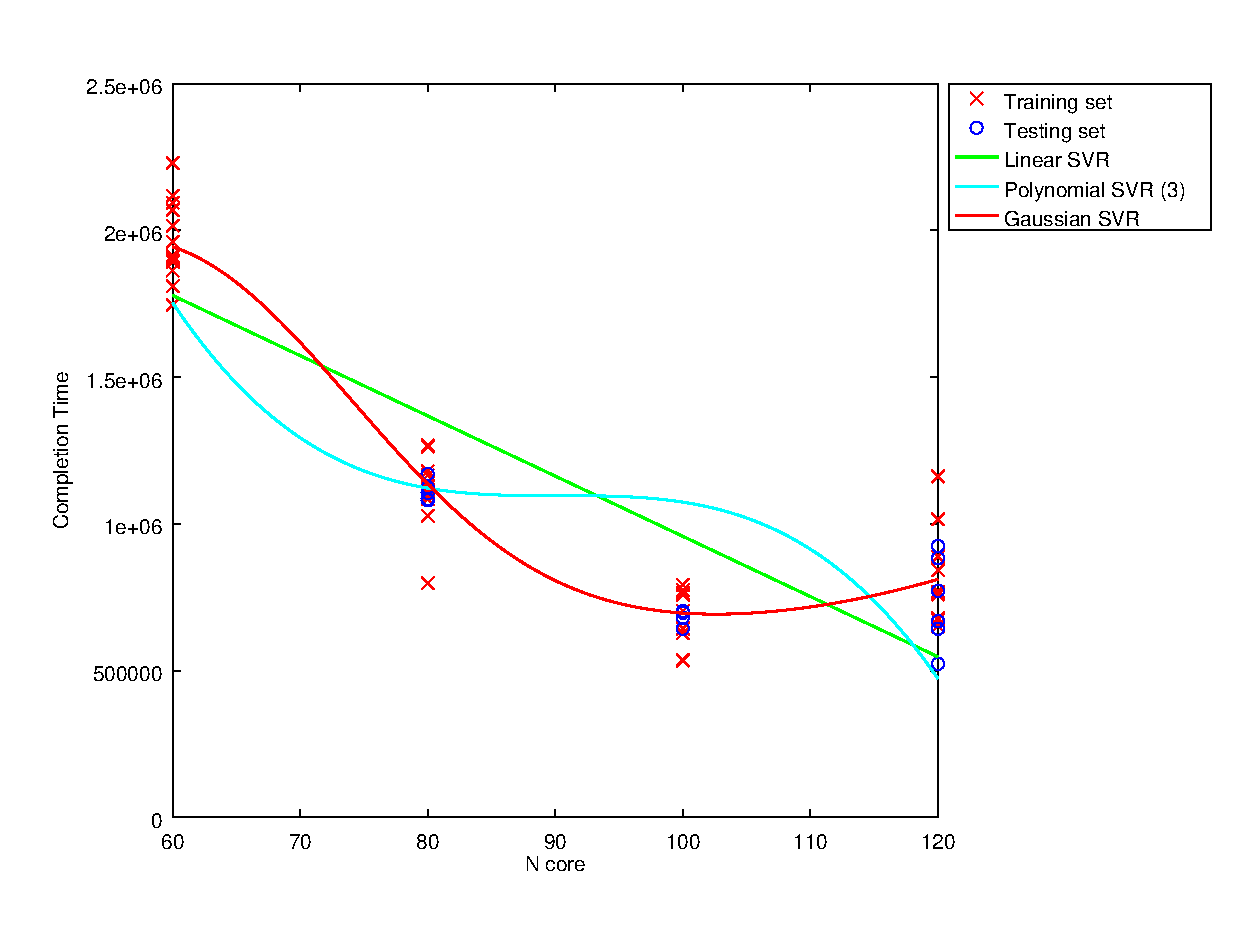
\includegraphics[width=\textwidth]{output/R2_1000_ONLY_1_LINEAR_NCORE/plot_R2_1000_bestmodels.eps}
\caption{Completion time vs ncores for query R2 with datasize 1000}
\label{fig:coreonly_linear_R2_1000}
\end {figure}

\newpage
\subsection{Query R3}
\subsubsection{Query R3 -- Datasize 250}
\begin{table}[H]
	\centering
	\begin{adjustbox}{center}
		\begin{tabular}{c | c M{1.2cm} M{2.5cm} M{2.5cm} M{1.8cm}}
			Model & RMSE & R\textsuperscript{2} & Mean absolute error & Mean relative error & Mean difference \tabularnewline
			\hline
			Linear regression & 0.5664 & 0.7343 & 218173 & 0.8842 & -0.2177 \\
			Linear SVR & 0.7419 & 0.8058 & 227474 & 1.9607 & -0.1042 \\
			Polynomial SVR (2) & 1.1232 & 0.0518 & 251296 & 25.0240 & -0.3209 \\
			Polynomial SVR (3) & 0.6689 & 0.7611 & 224745 & 6.2864 & -0.1218 \\
			Polynomial SVR (4) & 1.0818 & 0.0654 & 250379 & 10.5097 & -0.0906 \\
			Polynomial SVR (6) & 1.0776 & 0.0830 & 250143 & 10.5079 & -0.0870 \\
			Gaussian SVR & 0.6532 & 0.8353 & 221799 & 1.1592 & -0.0336 \\
		\end{tabular}
	\end{adjustbox}
	\\
	\caption{Results for R3-250}
	\label{fig:coreonly_linear_R3_250}
\end{table}

\begin {figure}[hbtp]
\centering
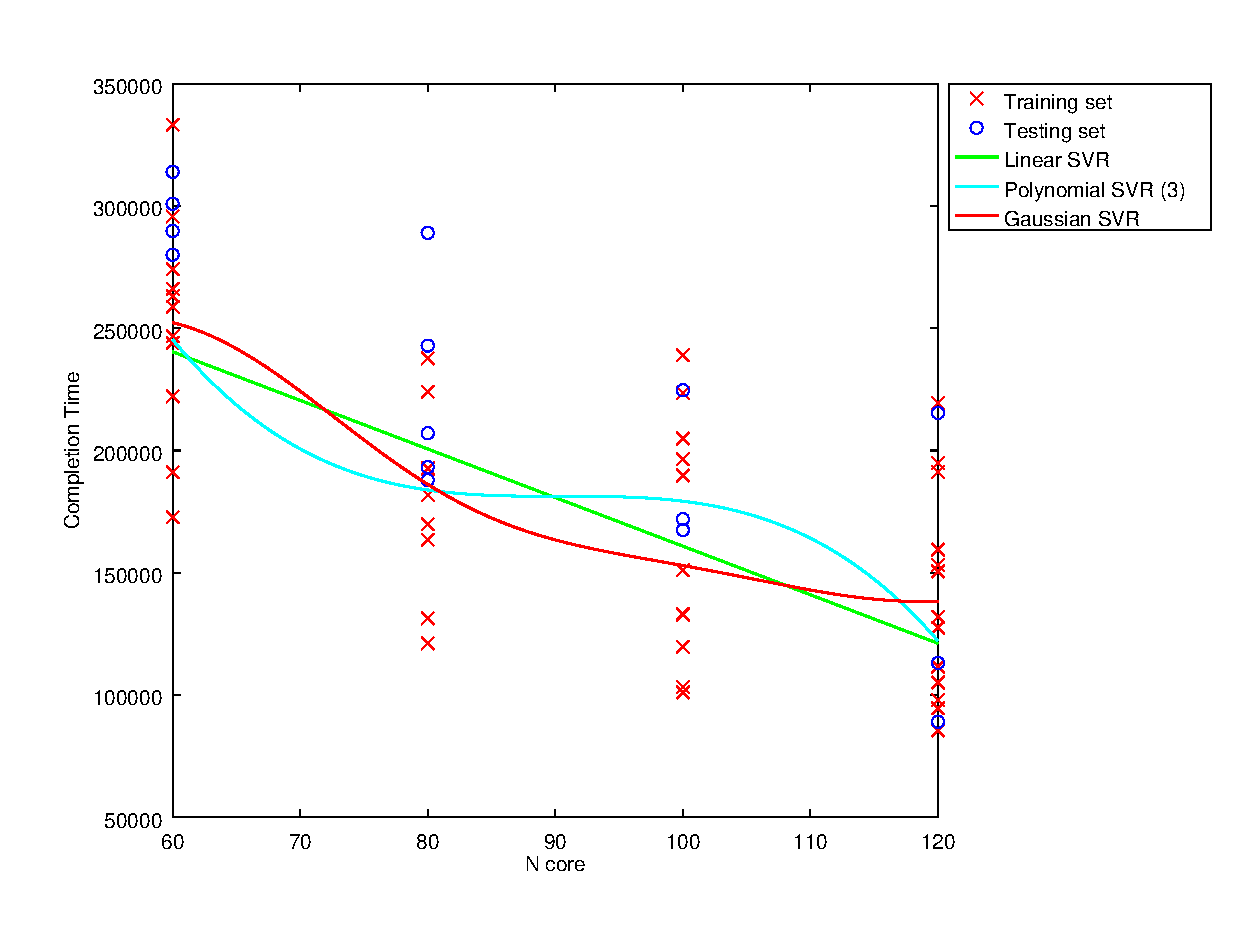
\includegraphics[width=\textwidth]{output/R3_250_ONLY_1_LINEAR_NCORE/plot_R3_250_bestmodels.eps}
\caption{Completion time vs ncores for query R3 with datasize 250}
\label{fig:coreonly_linear_R3_250}
\end {figure}

\newpage
\subsubsection{Query R3 -- Datasize 500}
\begin{table}[H]
	\centering
	\begin{adjustbox}{center}
		\begin{tabular}{c | c M{1.2cm} M{2.5cm} M{2.5cm} M{1.8cm}}
			Model & RMSE & R\textsuperscript{2} & Mean absolute error & Mean relative error & Mean difference \tabularnewline
			\hline
			Linear regression & 0.5105 & 0.7694 & 670050 & 0.7943 & -0.0100 \\
			Linear SVR & 0.5363 & 0.7945 & 671087 & 0.9138 & -0.1126 \\
			Polynomial SVR (2) & 1.2030 & 0.2948 & 759712 & 3.7549 & -0.4740 \\
			Polynomial SVR (3) & 0.5238 & 0.8230 & 665690 & 3.8134 & -0.1315 \\
			Polynomial SVR (4) & 1.2895 & 0.2034 & 764200 & 2.2969 & -0.5865 \\
			Polynomial SVR (6) & 1.2753 & 0.1148 & 761187 & 2.3991 & -0.5818 \\
			Gaussian SVR & 0.0857 & 0.9939 & 569642 & 0.2404 & -0.0176 \\
		\end{tabular}
	\end{adjustbox}
	\\
	\caption{Results for R3-500}
	\label{fig:coreonly_linear_R3_500}
\end{table}

\begin {figure}[hbtp]
\centering
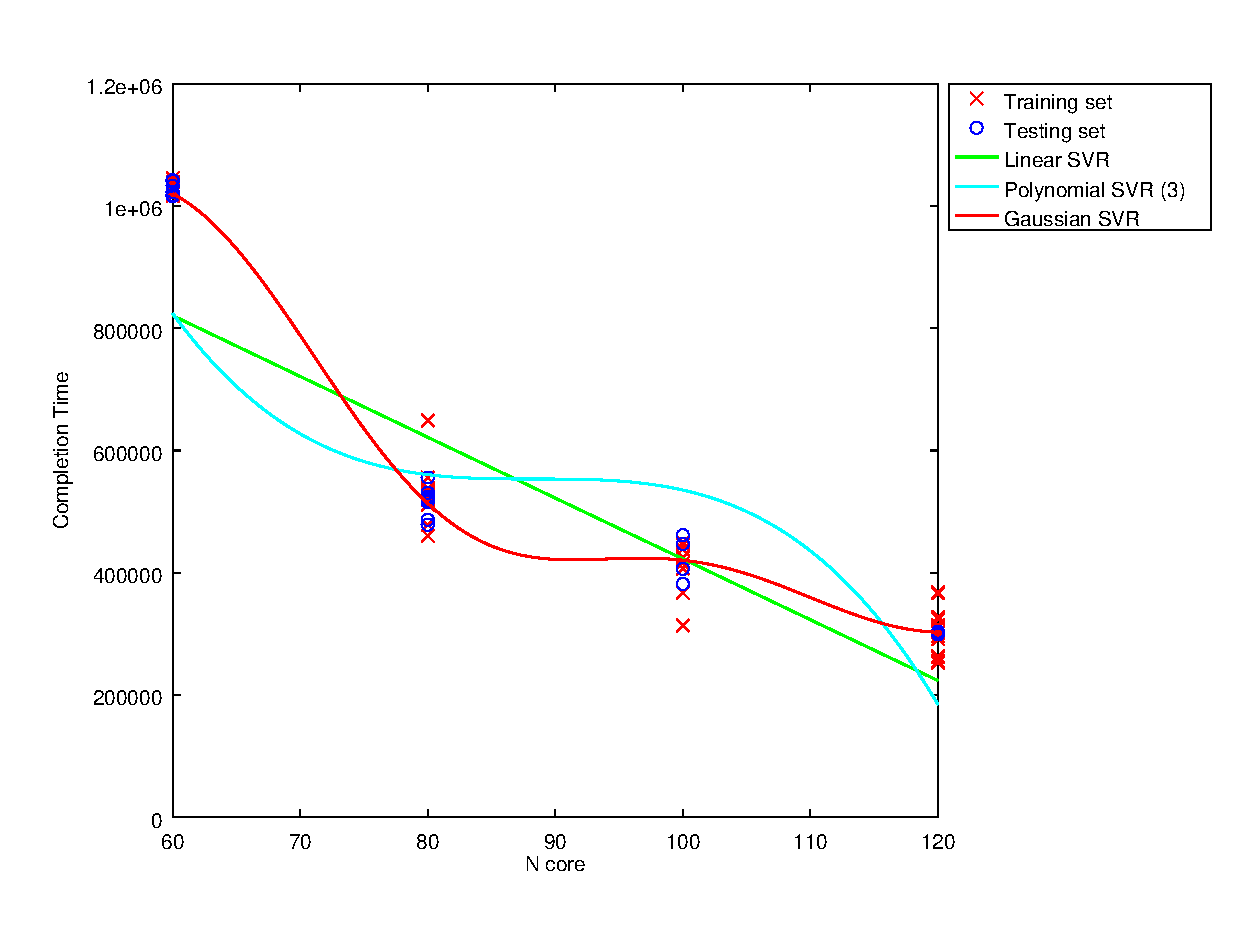
\includegraphics[width=\textwidth]{output/R3_500_ONLY_1_LINEAR_NCORE/plot_R3_500_bestmodels.eps}
\caption{Completion time vs ncores for query R3 with datasize 500}
\label{fig:coreonly_linear_R3_500}
\end {figure}

\newpage
\subsubsection{Query R3 -- Datasize 750}
\begin{table}[H]
	\centering
	\begin{adjustbox}{center}
		\begin{tabular}{c | c M{1.2cm} M{2.5cm} M{2.5cm} M{1.8cm}}
			Model & RMSE & R\textsuperscript{2} & Mean absolute error & Mean relative error & Mean difference \tabularnewline
			\hline
			Linear regression & 0.3758 & 0.8659 & 834166 & 0.4393 & -0.1866 \\
			Linear SVR & 0.4126 & 0.9086 & 834817 & 0.4707 & -0.2649 \\
			Polynomial SVR (2) & 1.2743 & 0.0000 & 959740 & 1.6523 & 0.5658 \\
			Polynomial SVR (3) & 0.5313 & 0.8931 & 857338 & 0.9029 & -0.4105 \\
			Polynomial SVR (4) & 1.2419 & 0.0035 & 953661 & 2.3823 & 0.5559 \\
			Polynomial SVR (6) & 1.1462 & 0.0137 & 941681 & 2.4817 & 0.4486 \\
			Gaussian SVR & 0.1570 & 0.9928 & 794470 & 0.2633 & 0.0987 \\
		\end{tabular}
	\end{adjustbox}
	\\
	\caption{Results for R3-750}
	\label{fig:coreonly_linear_R3_750}
\end{table}

\begin {figure}[hbtp]
\centering
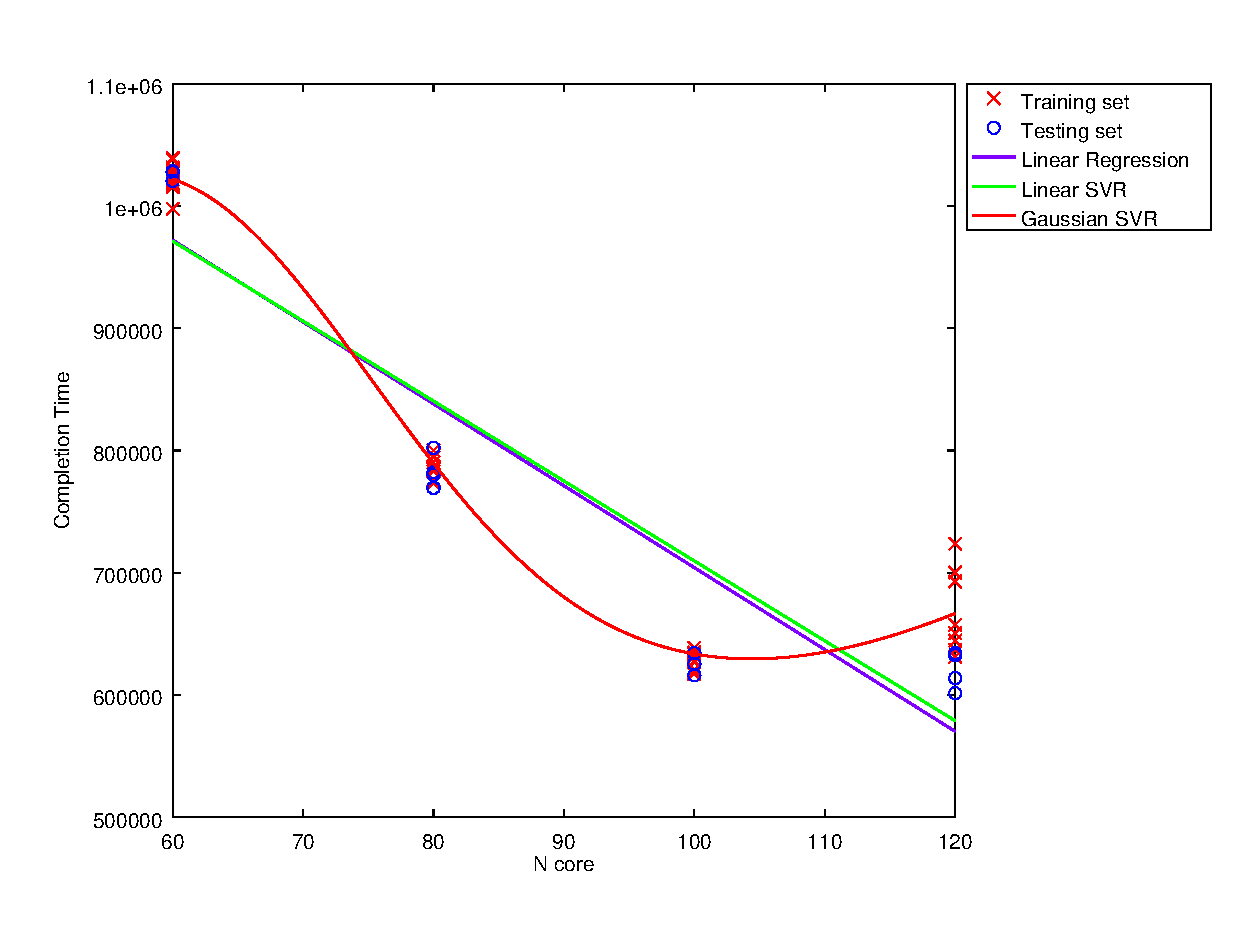
\includegraphics[width=\textwidth]{output/R3_750_ONLY_1_LINEAR_NCORE/plot_R3_750_bestmodels.eps}
\caption{Completion time vs ncores for query R3 with datasize 750}
\label{fig:coreonly_linear_R3_750}
\end {figure}

\newpage
\subsubsection{Query R3 -- Datasize 1000}
\begin{table}[H]
	\centering
	\begin{adjustbox}{center}
		\begin{tabular}{c | c M{1.2cm} M{2.5cm} M{2.5cm} M{1.8cm}}
			Model & RMSE & R\textsuperscript{2} & Mean absolute error & Mean relative error & Mean difference \tabularnewline
			\hline
			Linear regression & 0.4194 & 0.8055 & 1094689 & 0.6156 & -0.0390 \\
			Linear SVR & 0.4203 & 0.8082 & 1095259 & 0.6260 & -0.0178 \\
			Polynomial SVR (2) & 0.9347 & 0.0904 & 1186674 & 2.2891 & 0.2124 \\
			Polynomial SVR (3) & 0.5406 & 0.6895 & 1105677 & 61.6506 & 0.0900 \\
			Polynomial SVR (4) & 1.0026 & 0.0854 & 1197870 & 3.6921 & 0.4202 \\
			Polynomial SVR (6) & 1.0073 & 0.0796 & 1198563 & 3.6827 & 0.4237 \\
			Gaussian SVR & 0.1259 & 0.9834 & 1029516 & 0.1996 & -0.0218 \\
		\end{tabular}
	\end{adjustbox}
	\\
	\caption{Results for R3-1000}
	\label{fig:coreonly_linear_R3_1000}
\end{table}

\begin {figure}[hbtp]
\centering
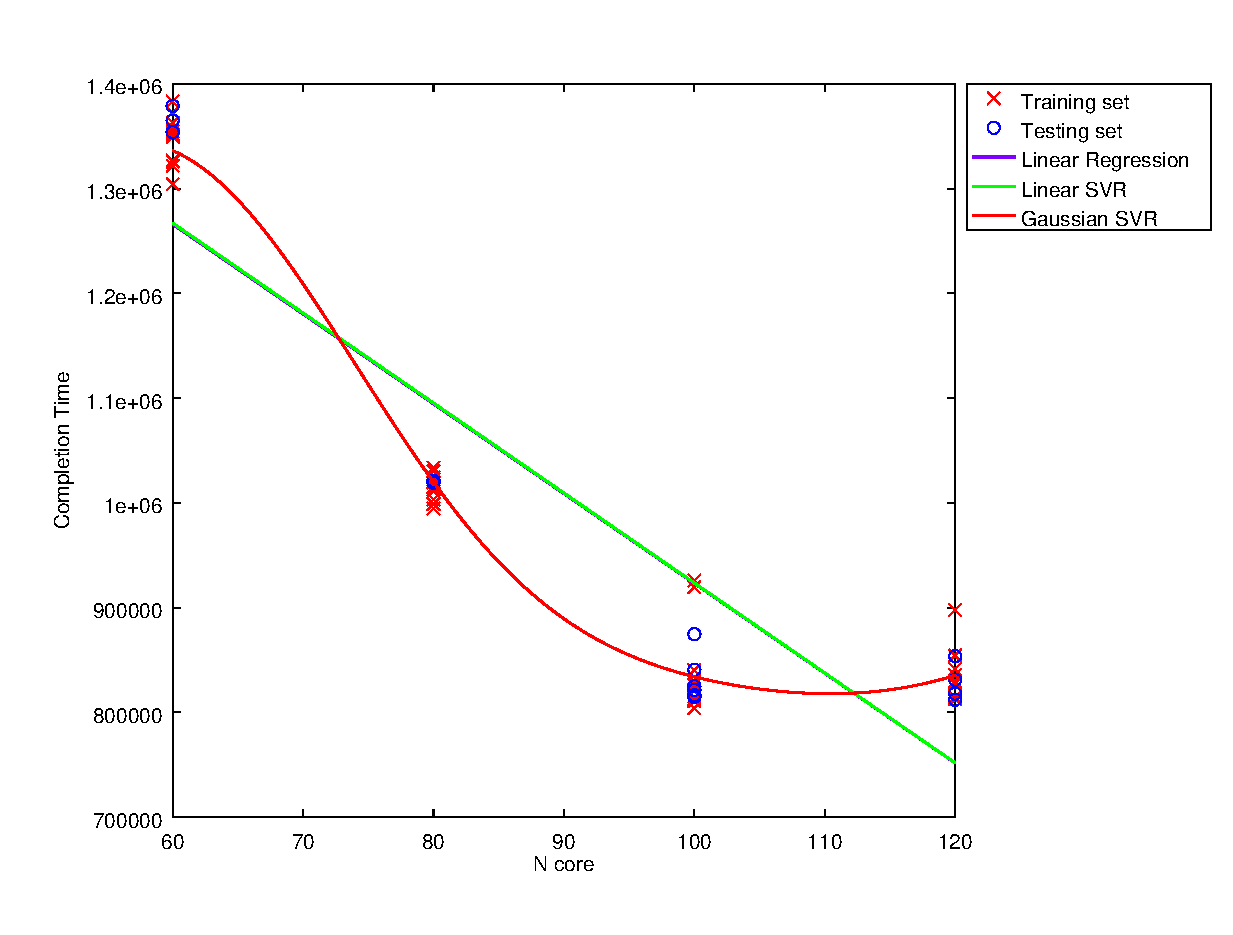
\includegraphics[width=\textwidth]{output/R3_1000_ONLY_1_LINEAR_NCORE/plot_R3_1000_bestmodels.eps}
\caption{Completion time vs ncores for query R3 with datasize 1000}
\label{fig:coreonly_linear_R3_1000}
\end {figure}

\newpage
\subsection{Query R4}
\subsubsection{Query R4 -- Datasize 250}
\begin{table}[H]
	\centering
	\begin{adjustbox}{center}
		\begin{tabular}{c | c M{1.2cm} M{2.5cm} M{2.5cm} M{1.8cm}}
			Model & RMSE & R\textsuperscript{2} & Mean absolute error & Mean relative error & Mean difference \tabularnewline
			\hline
			Linear regression & 0.5465 & 0.6549 & 165901 & 0.8526 & -0.1000 \\
			Linear SVR & 0.5680 & 0.6694 & 167035 & 1.0912 & -0.0712 \\
			Polynomial SVR (2) & 0.9898 & 0.2418 & 184689 & 12.6648 & -0.0528 \\
			Polynomial SVR (3) & 0.6954 & 0.5387 & 170652 & 4.5525 & -0.2458 \\
			Polynomial SVR (4) & 0.9815 & 0.1822 & 182938 & 9.2999 & 0.0814 \\
			Polynomial SVR (6) & 1.0310 & 0.1063 & 185998 & 17.8055 & -0.0432 \\
			Gaussian SVR & 0.5537 & 0.6586 & 165610 & 1.9384 & -0.0821 \\
		\end{tabular}
	\end{adjustbox}
	\\
	\caption{Results for R4-250}
	\label{fig:coreonly_linear_R4_250}
\end{table}

\begin {figure}[hbtp]
\centering
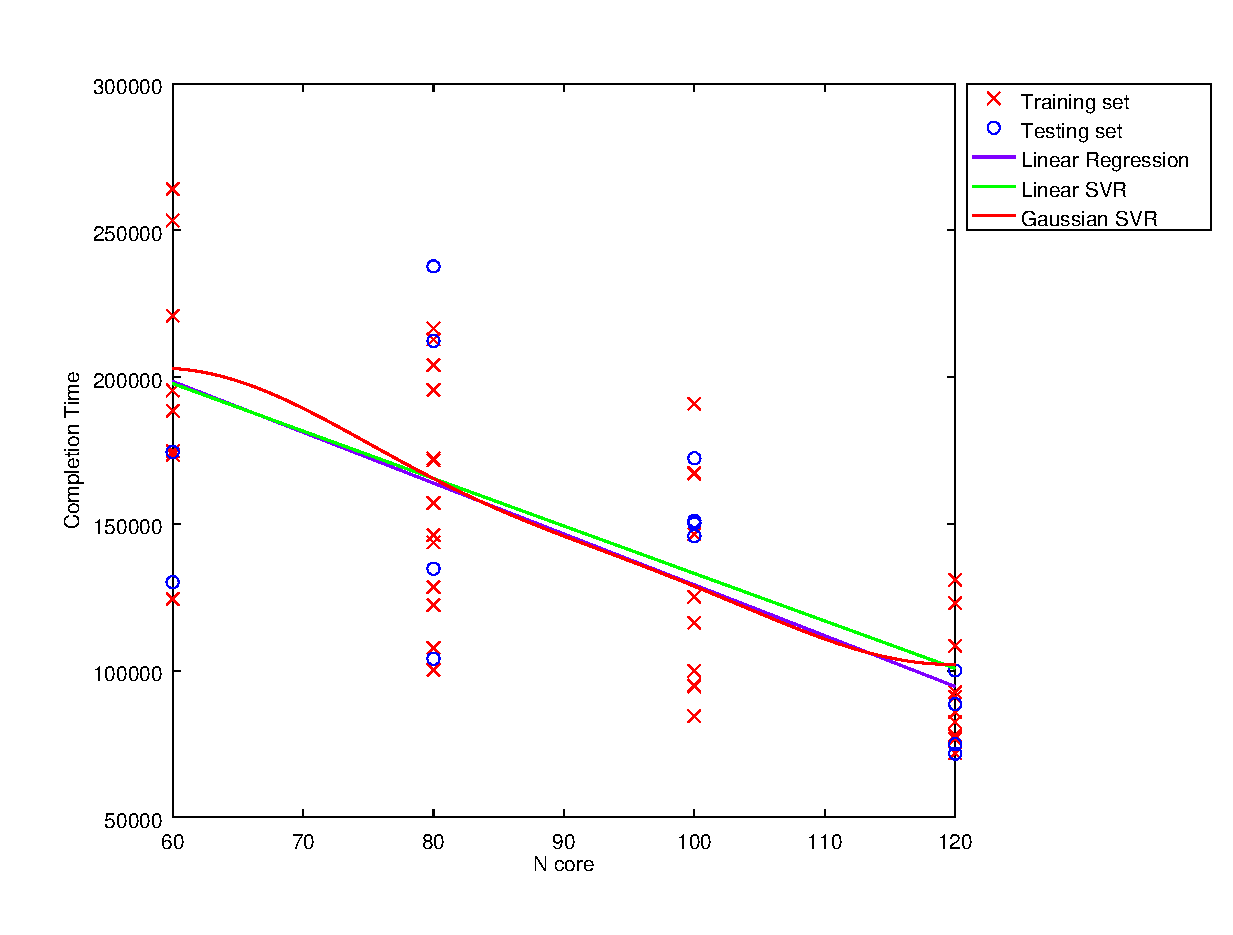
\includegraphics[width=\textwidth]{output/R4_250_ONLY_1_LINEAR_NCORE/plot_R4_250_bestmodels.eps}
\caption{Completion time vs ncores for query R4 with datasize 250}
\label{fig:coreonly_linear_R4_250}
\end {figure}

\newpage
\subsubsection{Query R4 -- Datasize 500}
\begin{table}[H]
	\centering
	\begin{adjustbox}{center}
		\begin{tabular}{c | c M{1.2cm} M{2.5cm} M{2.5cm} M{1.8cm}}
			Model & RMSE & R\textsuperscript{2} & Mean absolute error & Mean relative error & Mean difference \tabularnewline
			\hline
			Linear regression & 0.4870 & -0.9682 & 519719 & 0.8143 & 0.1174 \\
			Linear SVR & 0.3741 & 0.6131 & 501668 & 0.8938 & 0.0839 \\
			Polynomial SVR (2) & 0.5943 & 0.4650 & 511952 & 1.9030 & 0.3440 \\
			Polynomial SVR (3) & 0.4785 & 0.4615 & 513181 & 8.3968 & 0.1791 \\
			Polynomial SVR (4) & 0.5385 & 0.4285 & 522766 & 6.1419 & 0.4602 \\
			Polynomial SVR (6) & 0.5614 & 0.4212 & 528365 & 3.9017 & 0.4911 \\
			Gaussian SVR & 0.2286 & 0.6072 & 465503 & 0.2974 & -0.0529 \\
		\end{tabular}
	\end{adjustbox}
	\\
	\caption{Results for R4-500}
	\label{fig:coreonly_linear_R4_500}
\end{table}

\begin {figure}[hbtp]
\centering
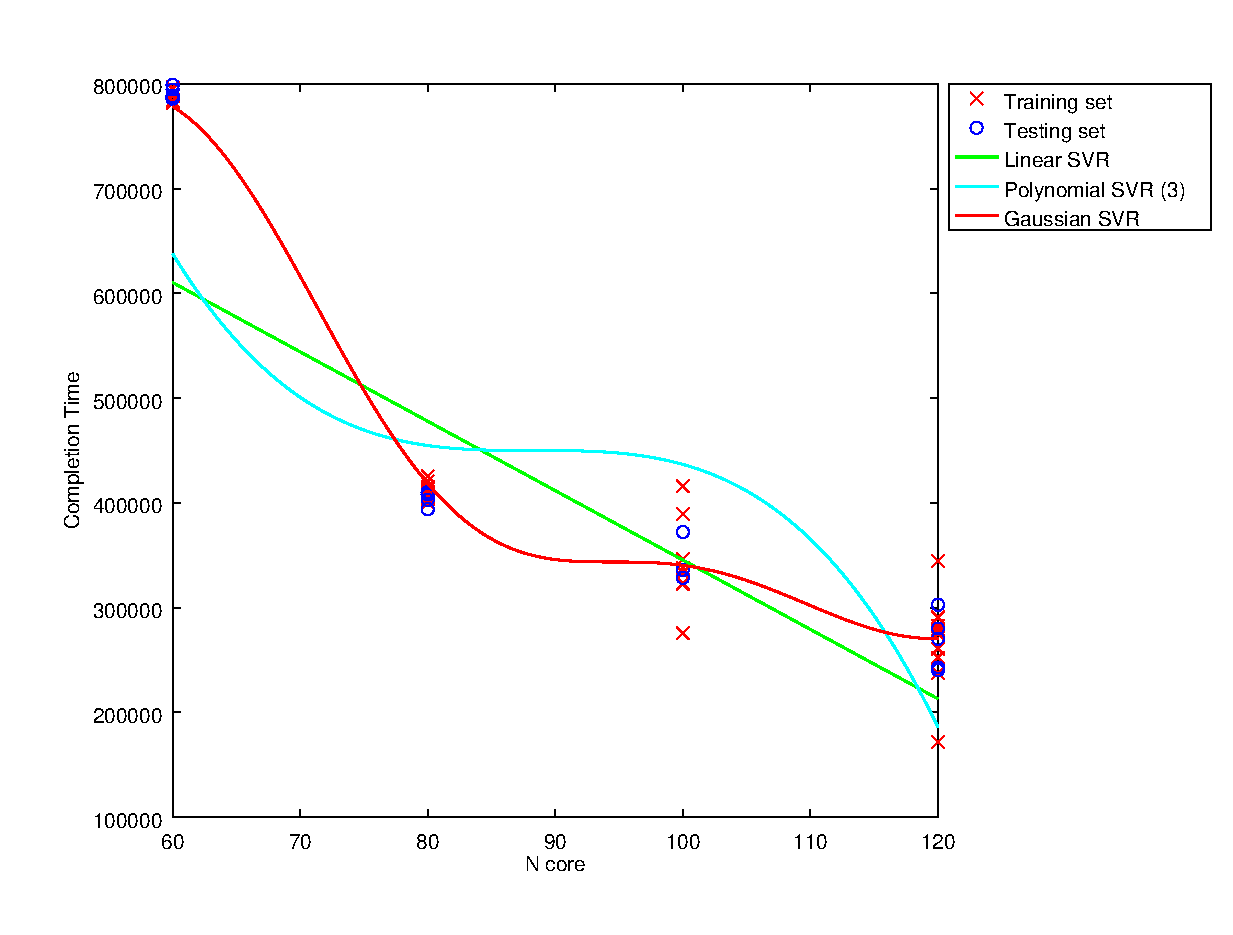
\includegraphics[width=\textwidth]{output/R4_500_ONLY_1_LINEAR_NCORE/plot_R4_500_bestmodels.eps}
\caption{Completion time vs ncores for query R4 with datasize 500}
\label{fig:coreonly_linear_R4_500}
\end {figure}

\newpage
\subsubsection{Query R4 -- Datasize 750}
\begin{table}[H]
	\centering
	\begin{adjustbox}{center}
		\begin{tabular}{c | c M{1.2cm} M{2.5cm} M{2.5cm} M{1.8cm}}
			Model & RMSE & R\textsuperscript{2} & Mean absolute error & Mean relative error & Mean difference \tabularnewline
			\hline
			Linear regression & 0.4796 & 0.7842 & 665860 & 0.4782 & -0.2843 \\
			Linear SVR & 0.4299 & 0.8858 & 660845 & 0.4889 & -0.2422 \\
			Polynomial SVR (2) & 1.2544 & 0.0006 & 751087 & 1.5979 & 0.5369 \\
			Polynomial SVR (3) & 0.6072 & 0.8817 & 681405 & 0.8451 & -0.4905 \\
			Polynomial SVR (4) & 1.2062 & 0.0009 & 744379 & 3.9300 & 0.5079 \\
			Polynomial SVR (6) & 1.2406 & 0.0079 & 747721 & 3.9595 & 0.5350 \\
			Gaussian SVR & 0.1315 & 0.9867 & 620515 & 0.2601 & -0.0488 \\
		\end{tabular}
	\end{adjustbox}
	\\
	\caption{Results for R4-750}
	\label{fig:coreonly_linear_R4_750}
\end{table}

\begin {figure}[hbtp]
\centering
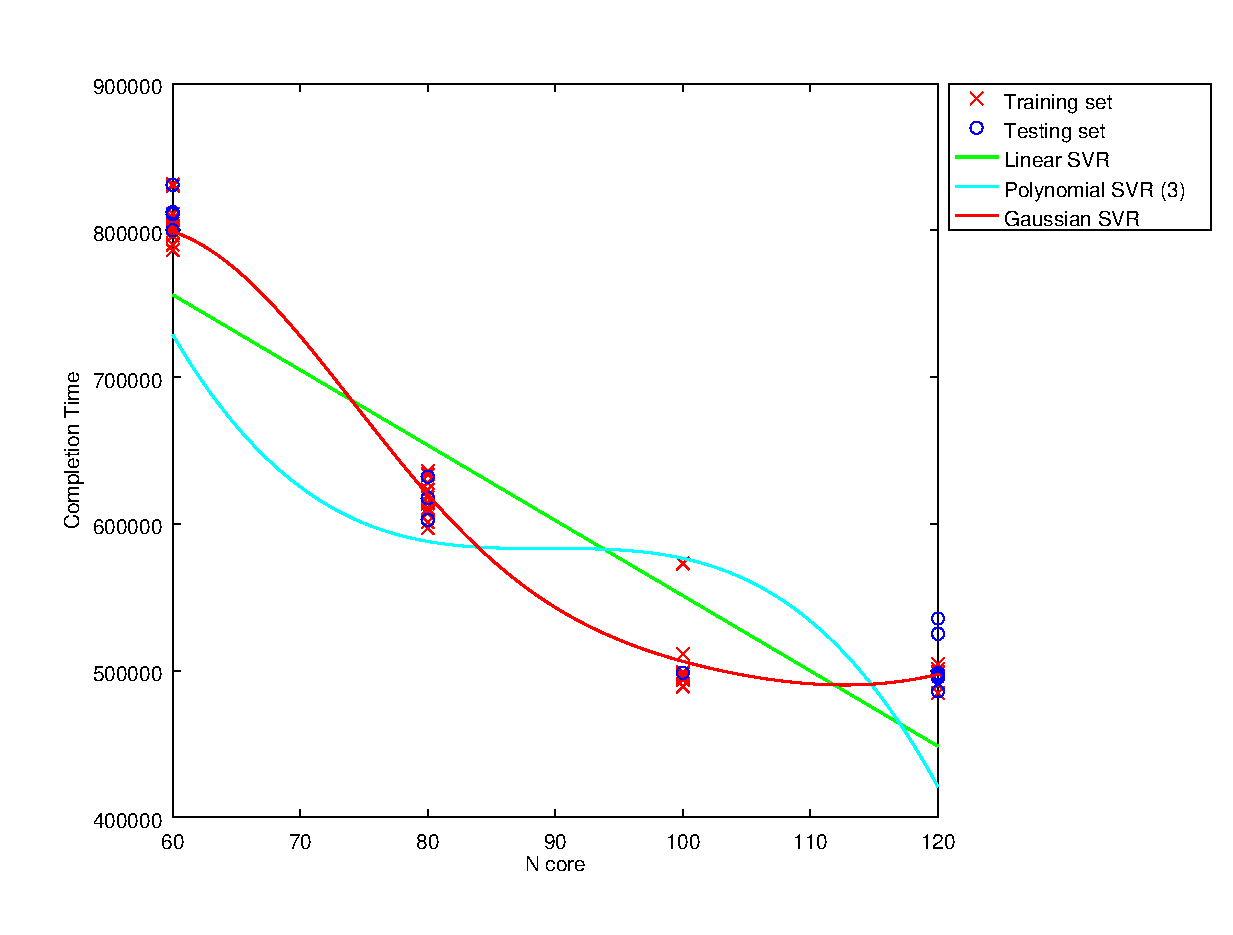
\includegraphics[width=\textwidth]{output/R4_750_ONLY_1_LINEAR_NCORE/plot_R4_750_bestmodels.eps}
\caption{Completion time vs ncores for query R4 with datasize 750}
\label{fig:coreonly_linear_R4_750}
\end {figure}

\newpage
\subsubsection{Query R4 -- Datasize 1000}
\begin{table}[H]
	\centering
	\begin{adjustbox}{center}
		\begin{tabular}{c | c M{1.2cm} M{2.5cm} M{2.5cm} M{1.8cm}}
			Model & RMSE & R\textsuperscript{2} & Mean absolute error & Mean relative error & Mean difference \tabularnewline
			\hline
			Linear regression & 0.5953 & 0.6065 & 2256524 & 1.0838 & -0.0301 \\
			Linear SVR & 0.6276 & 0.6095 & 2210275 & 1.4608 & 0.2046 \\
			Polynomial SVR (2) & 0.9265 & 0.0485 & 2524263 & 7.2145 & 0.0283 \\
			Polynomial SVR (3) & 0.7427 & 0.4249 & 2292008 & 2.5018 & 0.1736 \\
			Polynomial SVR (4) & 0.9240 & 0.0540 & 2524220 & 7.5100 & 0.0366 \\
			Polynomial SVR (6) & 0.9199 & 0.0628 & 2523162 & 7.5533 & 0.0449 \\
			Gaussian SVR & 0.4845 & 0.7610 & 2071198 & 0.2998 & 0.1305 \\
		\end{tabular}
	\end{adjustbox}
	\\
	\caption{Results for R4-1000}
	\label{fig:coreonly_linear_R4_1000}
\end{table}

\begin {figure}[hbtp]
\centering
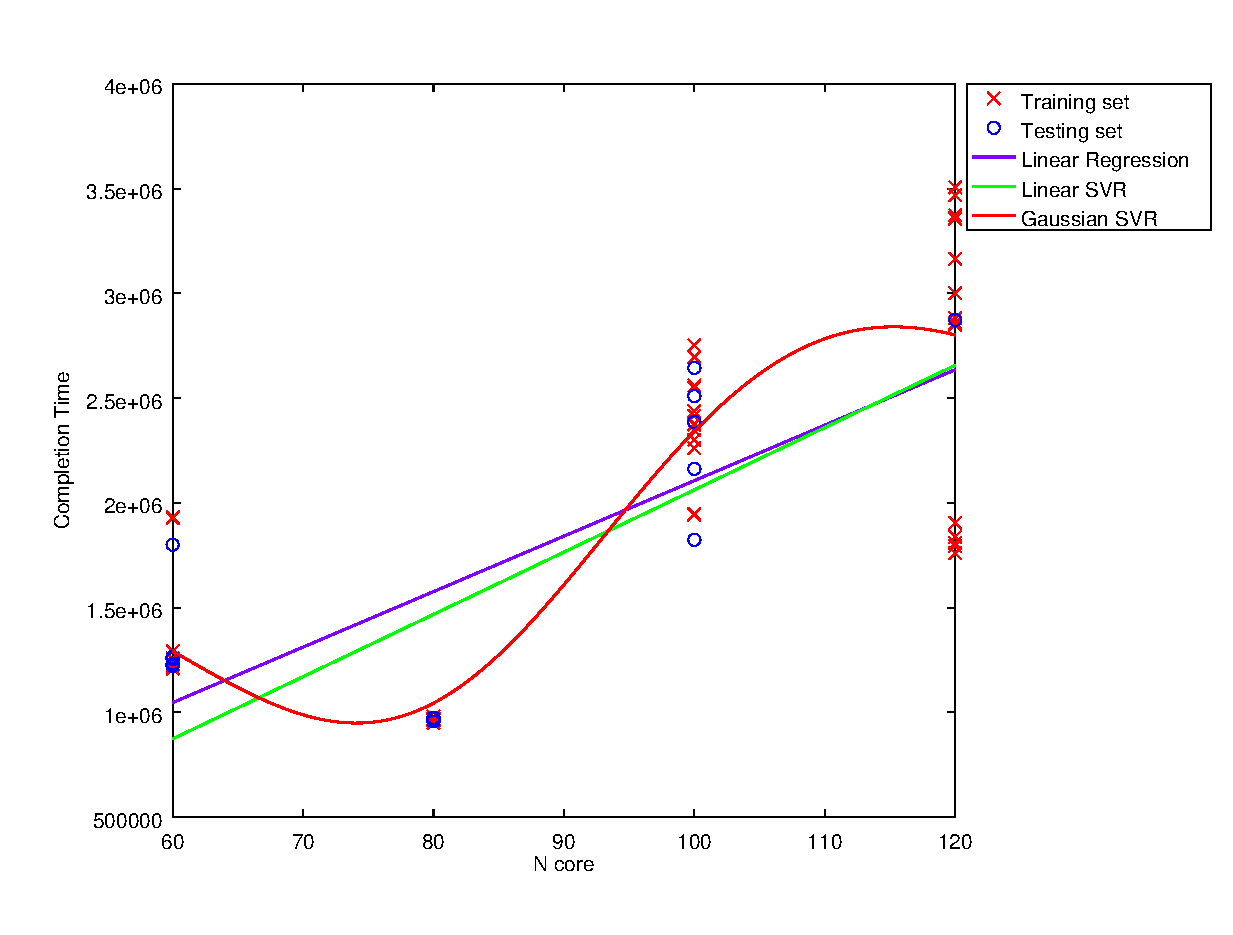
\includegraphics[width=\textwidth]{output/R4_1000_ONLY_1_LINEAR_NCORE/plot_R4_1000_bestmodels.eps}
\caption{Completion time vs ncores for query R4 with datasize 1000}
\label{fig:coreonly_linear_R4_1000}
\end {figure}

\newpage
\subsection{Query R5}
\subsubsection{Query R5 -- Datasize 250}
\begin{table}[H]
	\centering
	\begin{adjustbox}{center}
		\begin{tabular}{c | c M{1.2cm} M{2.5cm} M{2.5cm} M{1.8cm}}
			Model & RMSE & R\textsuperscript{2} & Mean absolute error & Mean relative error & Mean difference \tabularnewline
			\hline
			Linear regression & 0.7328 & 0.1952 &  25784 & 7.4799 & 0.1355 \\
			Linear SVR & 0.7999 & 0.2432 &  25846 & 11.8519 & -0.1475 \\
			Polynomial SVR (2) & 0.8293 & 0.0011 &  25888 & 15.1312 & -0.1350 \\
			Polynomial SVR (3) & 0.8399 & 0.2039 &  25888 & 12.9326 & -0.1059 \\
			Polynomial SVR (4) & 0.8305 & 0.0004 &  25890 & 16.2640 & -0.1345 \\
			Polynomial SVR (6) & 0.8322 & 0.0000 &  25892 & 14.7004 & -0.1373 \\
			Gaussian SVR & 0.7986 & 0.0547 &  25849 & 16.2030 & -0.0241 \\
		\end{tabular}
	\end{adjustbox}
	\\
	\caption{Results for R5-250}
	\label{fig:coreonly_linear_R5_250}
\end{table}

\begin {figure}[hbtp]
\centering
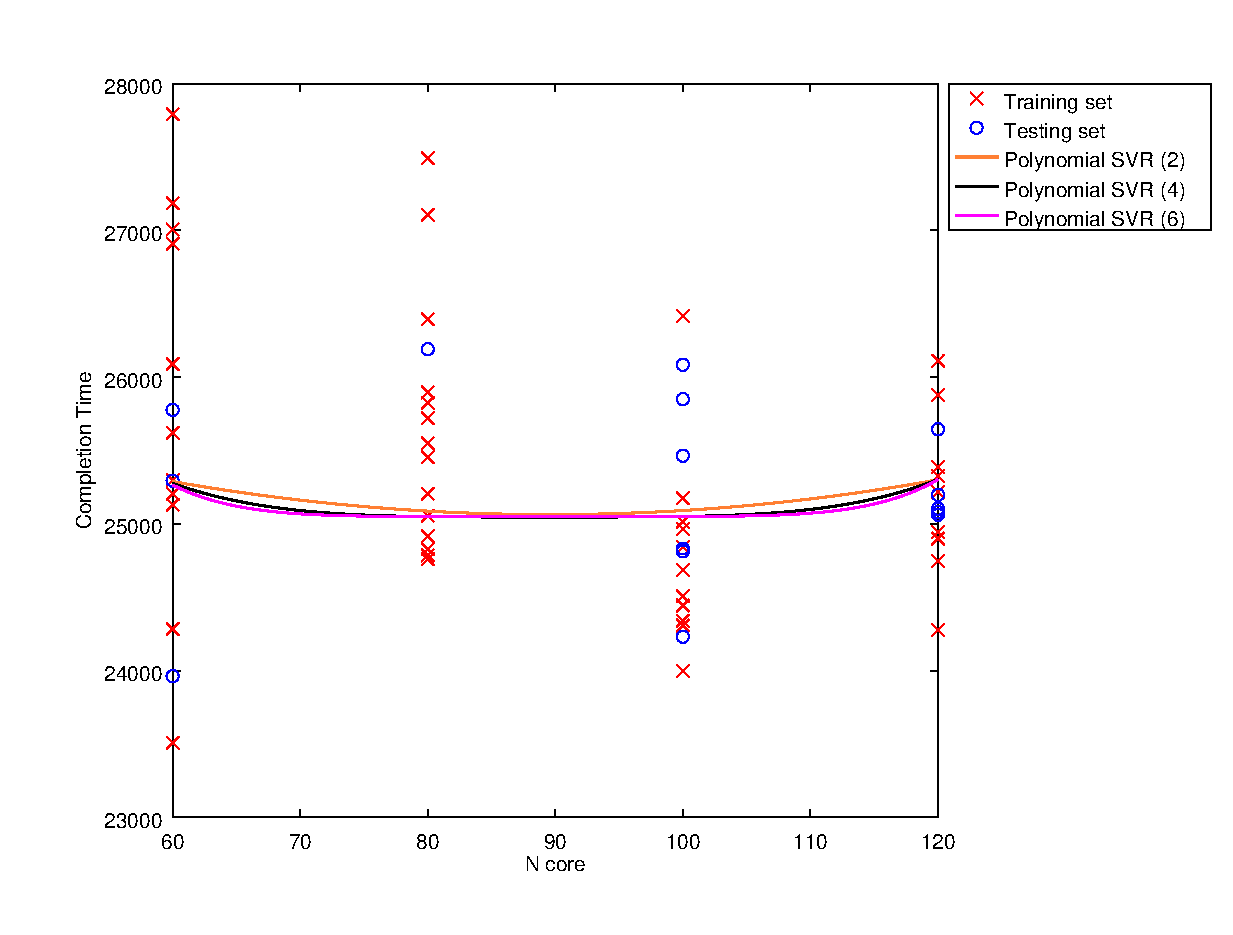
\includegraphics[width=\textwidth]{output/R5_250_ONLY_1_LINEAR_NCORE/plot_R5_250_bestmodels.eps}
\caption{Completion time vs ncores for query R5 with datasize 250}
\label{fig:coreonly_linear_R5_250}
\end {figure}

\newpage
\subsubsection{Query R5 -- Datasize 500}
\begin{table}[H]
	\centering
	\begin{adjustbox}{center}
		\begin{tabular}{c | c M{1.2cm} M{2.5cm} M{2.5cm} M{1.8cm}}
			Model & RMSE & R\textsuperscript{2} & Mean absolute error & Mean relative error & Mean difference \tabularnewline
			\hline
			Linear regression & 1.0764 & 0.0163 &  24770 & 5.8800 & -0.2806 \\
			Linear SVR & 1.1037 & 0.0931 &  24821 & 18.8609 & -0.3077 \\
			Polynomial SVR (2) & 1.2157 & 0.0001 &  24837 & 3.2243 & -0.4619 \\
			Polynomial SVR (3) & 1.1038 & 0.1516 &  24815 & 11.7193 & -0.3258 \\
			Polynomial SVR (4) & 1.2335 & 0.0054 &  24838 & 4.9444 & -0.5344 \\
			Polynomial SVR (6) & 1.1551 & 0.0177 &  24797 & 4.3414 & -0.4196 \\
			Gaussian SVR & 1.1236 & 0.0213 &  24807 & 6.4001 & -0.3311 \\
		\end{tabular}
	\end{adjustbox}
	\\
	\caption{Results for R5-500}
	\label{fig:coreonly_linear_R5_500}
\end{table}

\begin {figure}[hbtp]
\centering
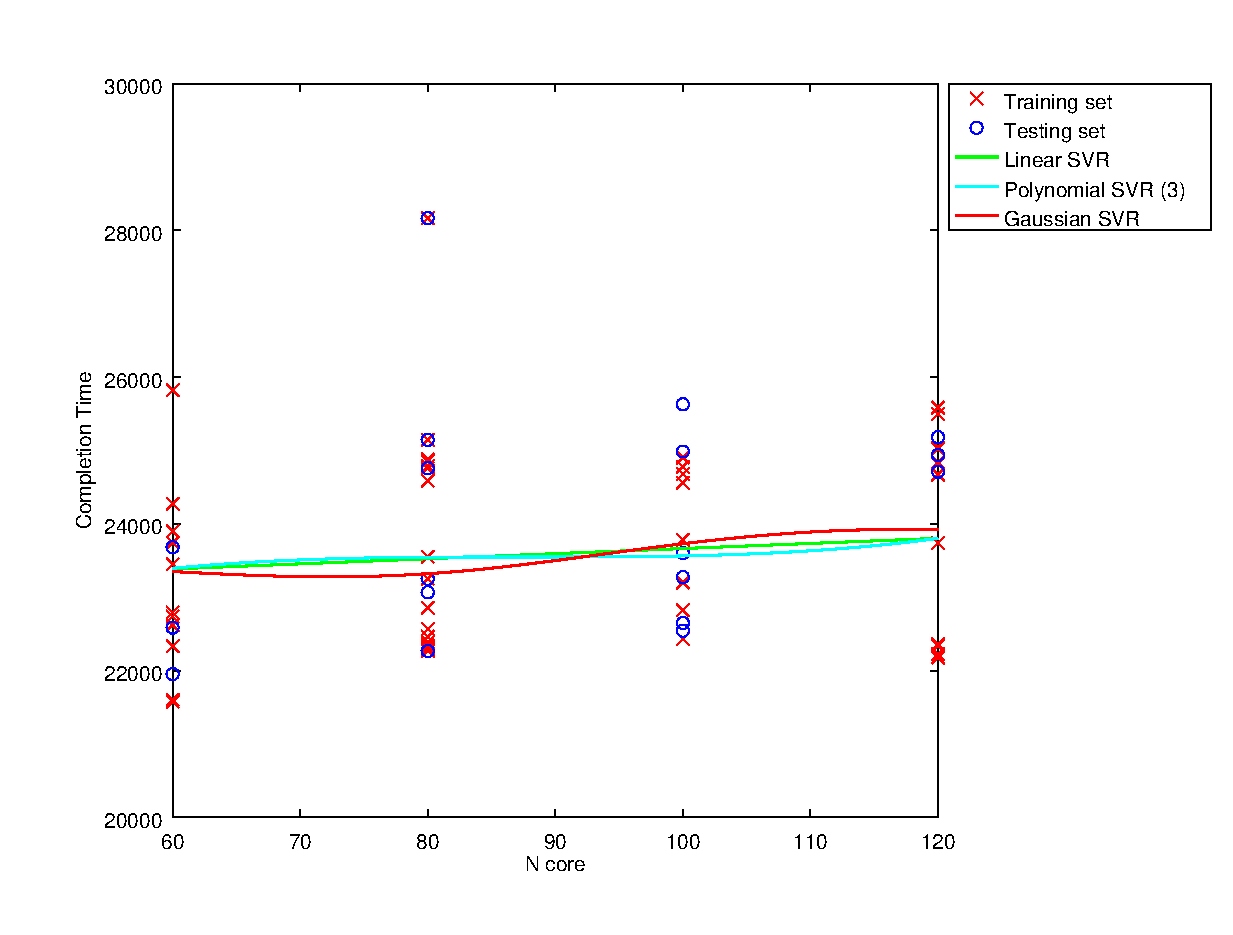
\includegraphics[width=\textwidth]{output/R5_500_ONLY_1_LINEAR_NCORE/plot_R5_500_bestmodels.eps}
\caption{Completion time vs ncores for query R5 with datasize 500}
\label{fig:coreonly_linear_R5_500}
\end {figure}

\newpage
\subsubsection{Query R5 -- Datasize 750}
\begin{table}[H]
	\centering
	\begin{adjustbox}{center}
		\begin{tabular}{c | c M{1.2cm} M{2.5cm} M{2.5cm} M{1.8cm}}
			Model & RMSE & R\textsuperscript{2} & Mean absolute error & Mean relative error & Mean difference \tabularnewline
			\hline
			Linear regression & 1.0876 & -0.1187 &  25108 & 14.6027 & -0.4073 \\
			Linear SVR & 1.1221 & 0.1018 &  25156 & 12.5852 & -0.5129 \\
			Polynomial SVR (2) & 1.1094 & 0.1066 &  25103 & 662.9814 & -0.4704 \\
			Polynomial SVR (3) & 1.1223 & 0.0909 &  25156 & 12.2314 & -0.5079 \\
			Polynomial SVR (4) & 1.1096 & 0.1091 &  25104 & 615.7160 & -0.4710 \\
			Polynomial SVR (6) & 1.1098 & 0.1119 &  25105 & 599.4620 & -0.4719 \\
			Gaussian SVR & 1.1222 & 0.1033 &  25156 & 12.9801 & -0.5144 \\
		\end{tabular}
	\end{adjustbox}
	\\
	\caption{Results for R5-750}
	\label{fig:coreonly_linear_R5_750}
\end{table}

\begin {figure}[hbtp]
\centering
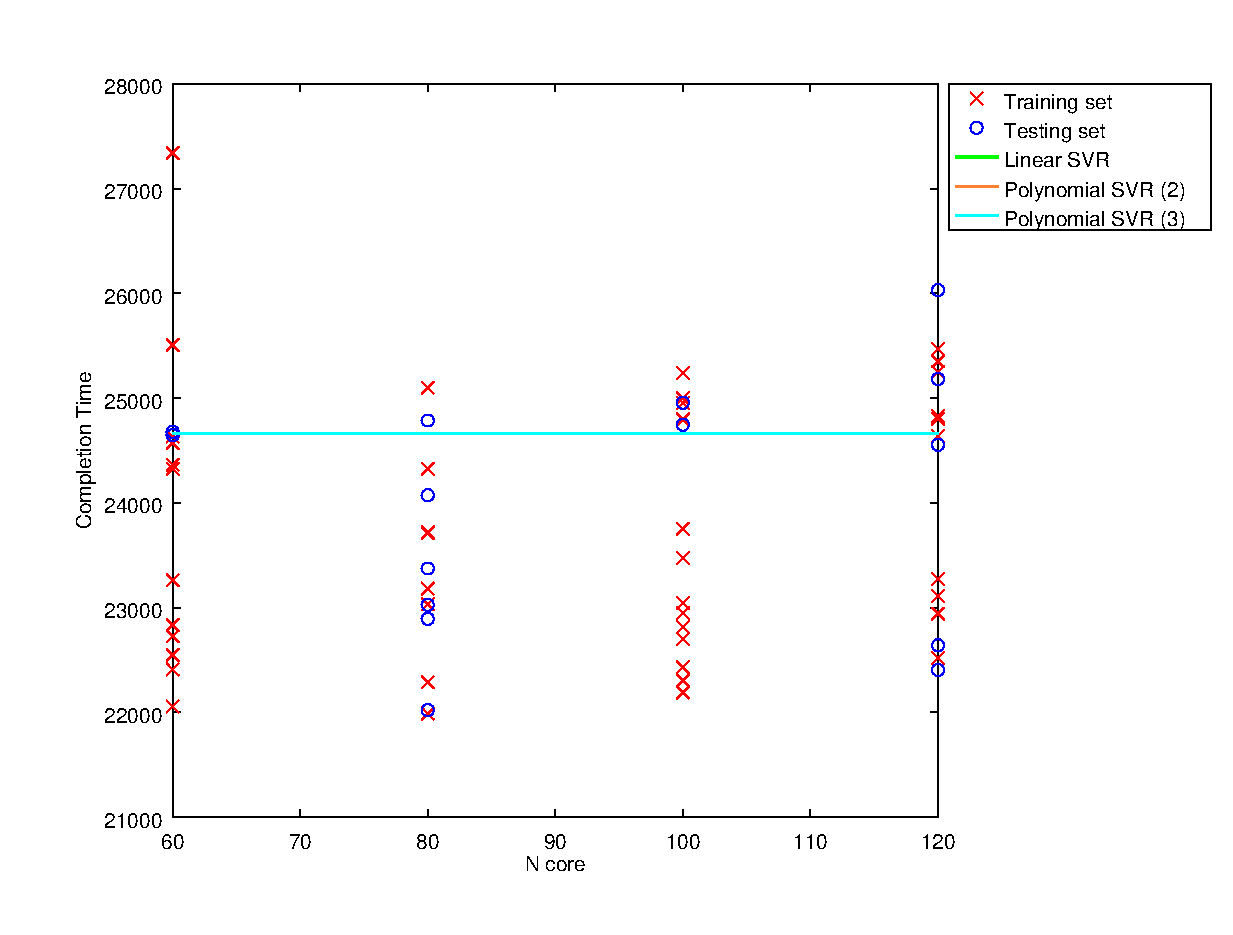
\includegraphics[width=\textwidth]{output/R5_750_ONLY_1_LINEAR_NCORE/plot_R5_750_bestmodels.eps}
\caption{Completion time vs ncores for query R5 with datasize 750}
\label{fig:coreonly_linear_R5_750}
\end {figure}

\newpage
\subsubsection{Query R5 -- Datasize 1000}
\begin{table}[H]
	\centering
	\begin{adjustbox}{center}
		\begin{tabular}{c | c M{1.2cm} M{2.5cm} M{2.5cm} M{1.8cm}}
			Model & RMSE & R\textsuperscript{2} & Mean absolute error & Mean relative error & Mean difference \tabularnewline
			\hline
			Linear regression & 1.1760 & 0.2105 &  43437 & 3.4328 & -0.3100 \\
			Linear SVR & 1.1734 & 0.3227 &  43479 & 3.3087 & -0.2301 \\
			Polynomial SVR (2) & 1.2608 & 0.1464 &  43434 & 3.6967 & -0.2246 \\
			Polynomial SVR (3) & 1.1189 & 0.4733 &  43178 & 14.3300 & -0.3185 \\
			Polynomial SVR (4) & 1.2150 & 0.2306 &  43271 & 3.1325 & -0.2220 \\
			Polynomial SVR (6) & 1.1549 & 0.3291 &  43120 & 2.8657 & -0.1946 \\
			Gaussian SVR & 1.0927 & 0.6095 &  43105 & 5.8926 & -0.2533 \\
		\end{tabular}
	\end{adjustbox}
	\\
	\caption{Results for R5-1000}
	\label{fig:coreonly_linear_R5_1000}
\end{table}

\begin {figure}[hbtp]
\centering
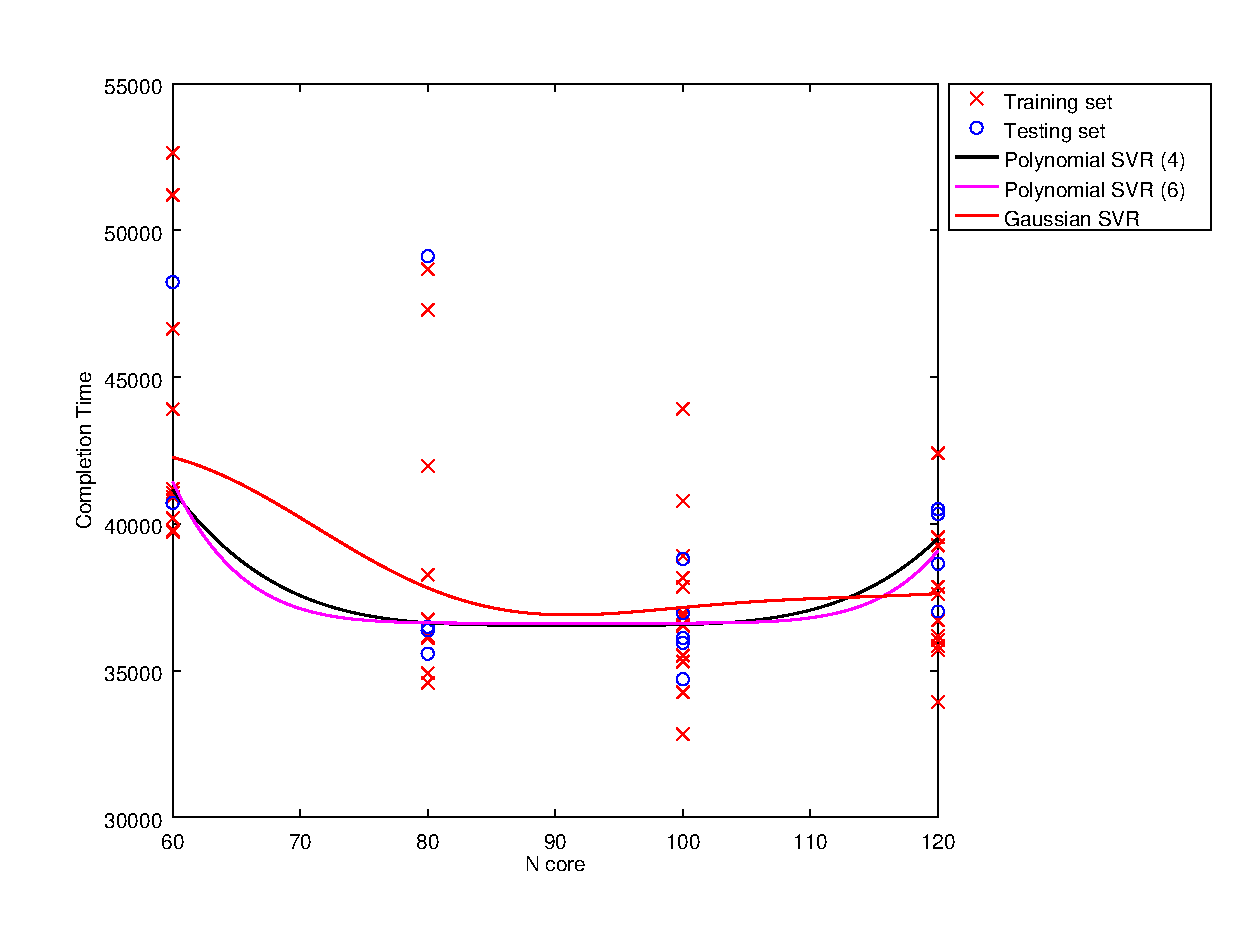
\includegraphics[width=\textwidth]{output/R5_1000_ONLY_1_LINEAR_NCORE/plot_R5_1000_bestmodels.eps}
\caption{Completion time vs ncores for query R5 with datasize 1000}
\label{fig:coreonly_linear_R5_1000}
\end {figure}

%-------------------------------------------

\newpage
\section{Fixed Datasize, $ncores^{-1}$, All the Features}
\subsection{Query R1}
\subsubsection{Query R1 -- Datasize 250}
\begin{table}[H]
	\centering
	\begin{adjustbox}{center}
		\begin{tabular}{c | c M{1.2cm} M{2.5cm} M{2.5cm} M{1.8cm}}
			Model & RMSE & R\textsuperscript{2} & Mean absolute error & Mean relative error & Mean difference \tabularnewline
			\hline
			Linear regression & 0.3569 & 0.9437 &  57917 & 0.1222 & -0.1020 \\
			Linear SVR & 0.3897 & 0.9727 &  58167 & 0.1350 & -0.1083 \\
			Polynomial SVR (2) & 0.7267 & 0.7759 &  66118 & 61.3335 & 0.1183 \\
			Polynomial SVR (3) & 3.6861 & 0.7898 &  76246 & 1.3885 & 1.1331 \\
			Polynomial SVR (4) & 2.1868 & 0.2291 &  74023 & 2.8312 & -0.6560 \\
			Polynomial SVR (6) & 3.1348 & 0.3153 &  80690 & 8.4469 & -1.0235 \\
			Gaussian SVR & 1.2154 & 0.4402 &  63043 & 2.3972 & -0.3644 \\
		\end{tabular}
	\end{adjustbox}
	\\
	\caption{Results for R1-250 with non-linear 1/ncores feature}
	\label{table_R1_prediction_all}
\end{table}

\begin {figure}[hbtp]
\centering
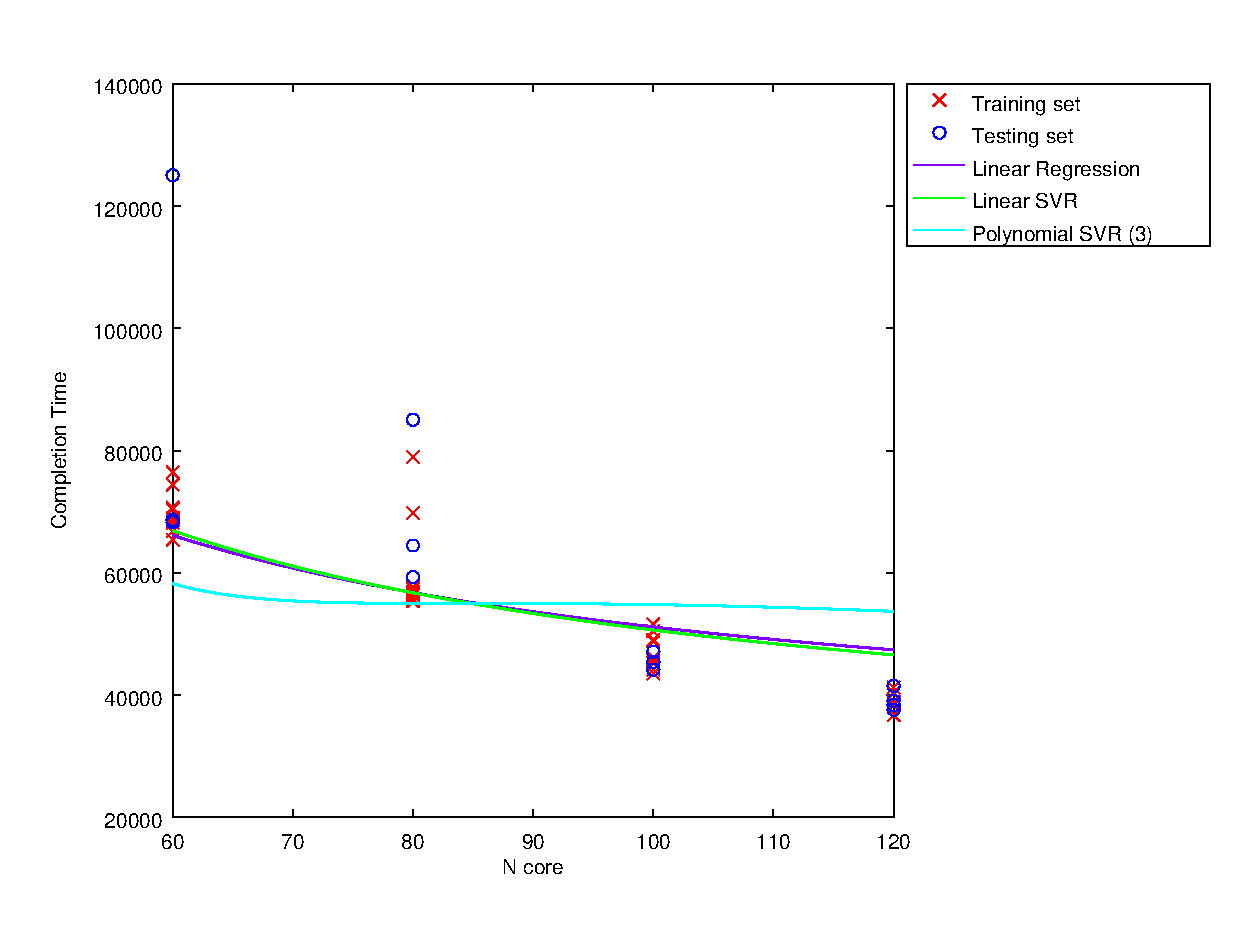
\includegraphics[width=\textwidth]{output/R1_250_NO_72_90_1_OVER_NCORES/plot_R1_250_bestmodels.eps}
\caption {Completion time vs ncores for query R1 with datasize 250}
\end {figure}

\newpage
\subsubsection{Query R1 -- Datasize 500}
\begin{table}[H]
	\centering
	\begin{adjustbox}{center}
		\begin{tabular}{c | c M{1.2cm} M{2.5cm} M{2.5cm} M{1.8cm}}
			Model & RMSE & R\textsuperscript{2} & Mean absolute error & Mean relative error & Mean difference \tabularnewline
			\hline
			Linear regression & 0.0506 & 0.9946 & 149372 & 1.1926 & -0.0195 \\
			Linear SVR & 0.0713 & 0.9903 & 151285 & 0.3085 & -0.0185 \\
			Polynomial SVR (2) & 0.4531 & 0.6440 & 168894 & 0.9474 & -0.0613 \\
			Polynomial SVR (3) & 0.2676 & 0.9424 & 159376 & 0.3461 & -0.0354 \\
			Polynomial SVR (4) & 0.5083 & 0.6031 & 169800 & 1.1381 & -0.0573 \\
			Polynomial SVR (6) & 0.5413 & 0.5082 & 172592 & 1.7399 & -0.0119 \\
			Gaussian SVR & 0.3465 & 0.8506 & 162296 & 0.9260 & -0.0197 \\
		\end{tabular}
	\end{adjustbox}
	\\
	\caption{Results for R1-500 with non-linear 1/ncores feature}
	\label{table_R1_prediction_all}
\end{table}

\begin {figure}[hbtp]
\centering
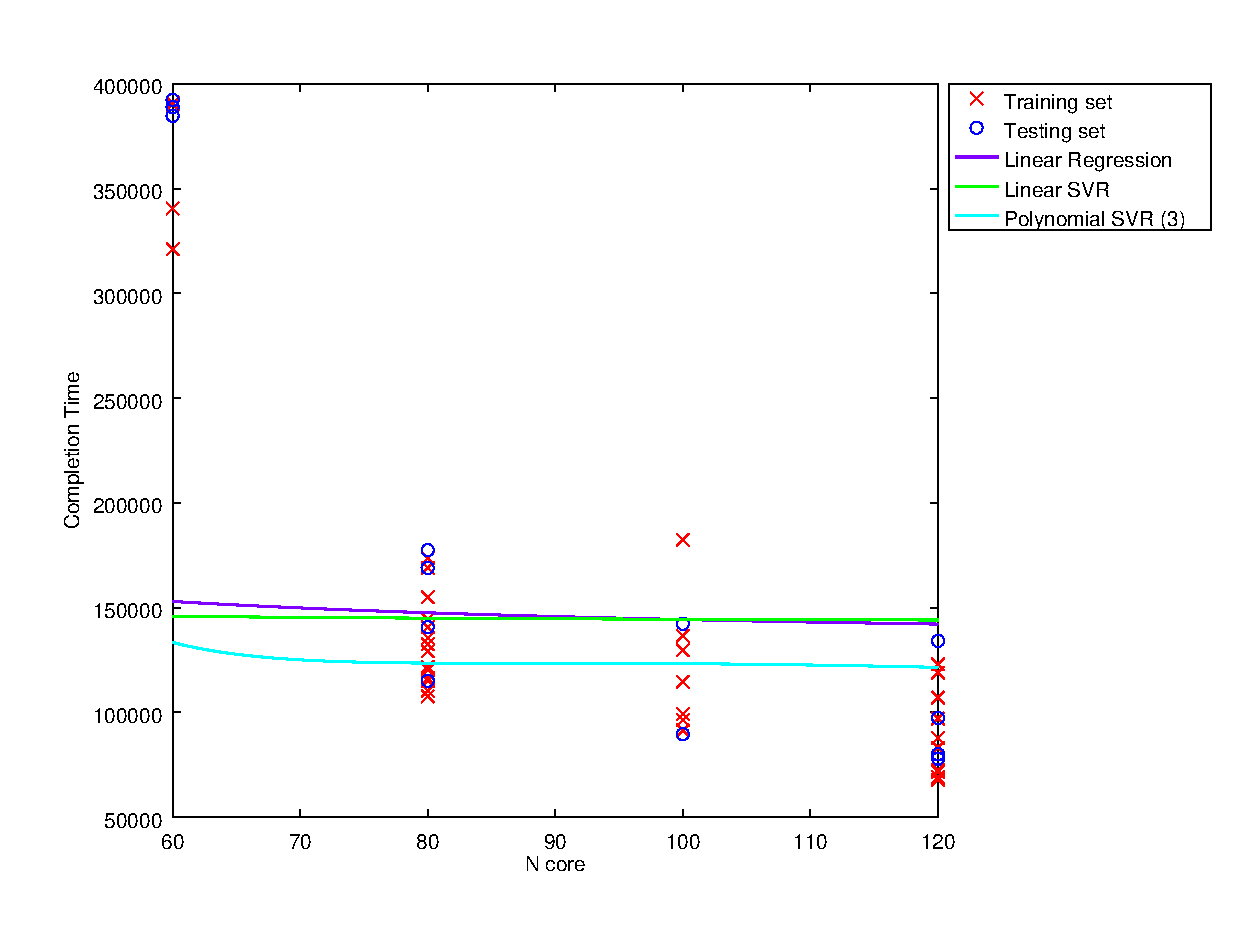
\includegraphics[width=\textwidth]{output/R1_500_1_OVER_NCORES/plot_R1_500_bestmodels.eps}
\caption {Completion time vs ncores for query R1 with datasize 500}
\end {figure}

\newpage
\subsubsection{Query R1 -- Datasize 750}
\begin{table}[H]
	\centering
	\begin{adjustbox}{center}
		\begin{tabular}{c | c M{1.2cm} M{2.5cm} M{2.5cm} M{1.8cm}}
			Model & RMSE & R\textsuperscript{2} & Mean absolute error & Mean relative error & Mean difference \tabularnewline
			\hline
			Linear regression & 0.1375 & 0.9744 & 266690 & 0.1768 & 0.0079 \\
			Linear SVR & 0.1334 & 0.9761 & 267032 & 0.1951 & 0.0088 \\
			Polynomial SVR (2) & 0.7191 & 0.3759 & 313187 & 6.5148 & 0.2147 \\
			Polynomial SVR (3) & 0.3711 & 0.8732 & 284595 & 1.1409 & 0.0472 \\
			Polynomial SVR (4) & 0.7398 & 0.3292 & 312671 & 15.8989 & 0.1402 \\
			Polynomial SVR (6) & 0.6509 & 0.4372 & 303665 & 3.8494 & -0.0005 \\
			Gaussian SVR & 0.2336 & 0.9523 & 272389 & 0.2649 & 0.1202 \\
		\end{tabular}
	\end{adjustbox}
	\\
	\caption{Results for R1-750 with non-linear 1/ncores feature}
	\label{table_R1_prediction_all}
\end{table}

\begin {figure}[hbtp]
\centering
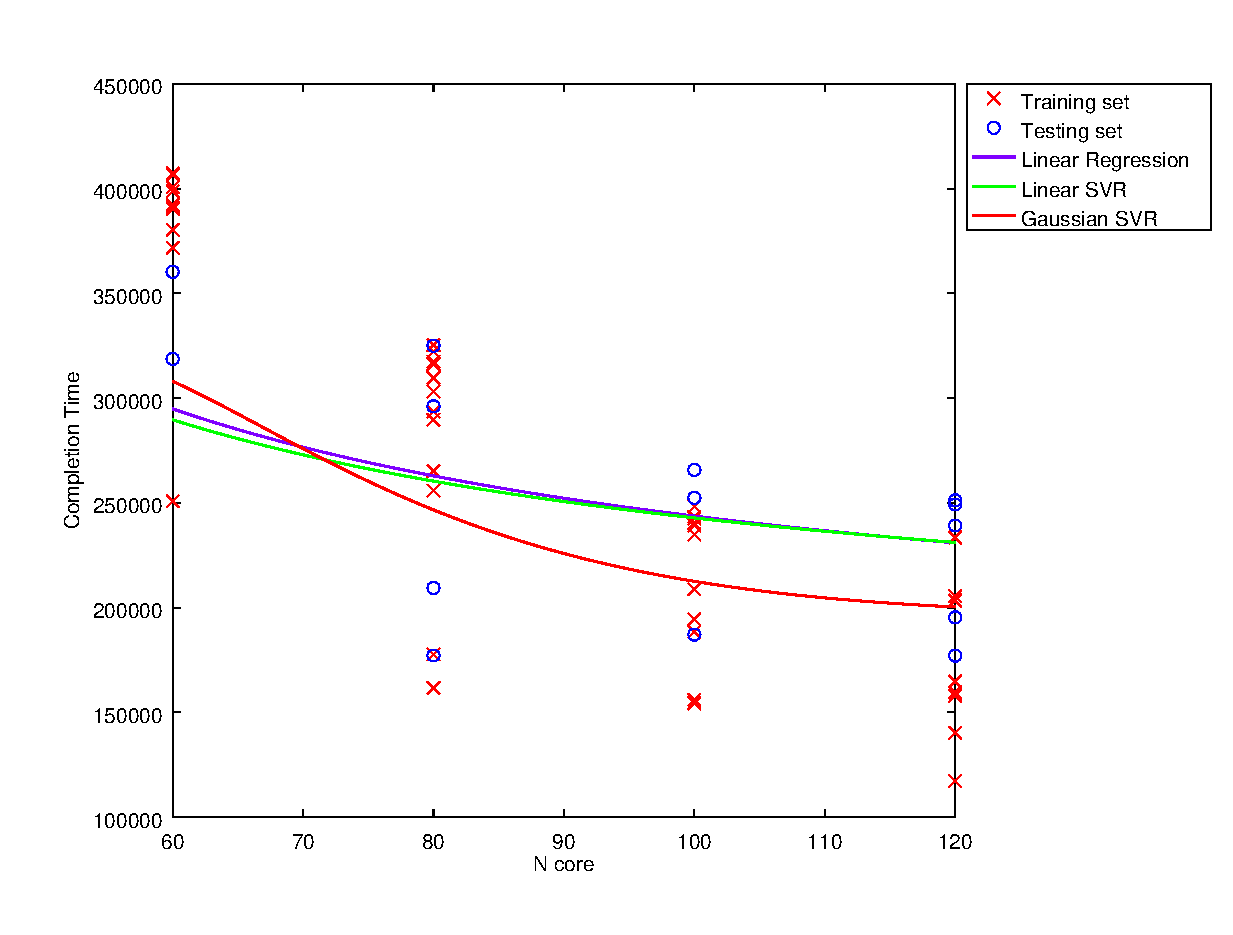
\includegraphics[width=\textwidth]{output/R1_750_1_OVER_NCORES/plot_R1_750_bestmodels.eps}
\caption {Completion time vs ncores for query R1 with datasize 750}
\end {figure}

\newpage
\subsubsection{Query R1 -- Datasize 1000}
\begin{table}[H]
	\centering
	\begin{adjustbox}{center}
		\begin{tabular}{c | c M{1.2cm} M{2.5cm} M{2.5cm} M{1.8cm}}
			Model & RMSE & R\textsuperscript{2} & Mean absolute error & Mean relative error & Mean difference \tabularnewline
			\hline
			Linear regression & 0.1306 & 0.9784 & 429351 & 2.8409 & 0.0007 \\
			Linear SVR & 0.1450 & 0.9810 & 429604 & 0.5520 & 0.0338 \\
			Polynomial SVR (2) & 0.8082 & 0.2162 & 482601 & 3.1941 & 0.0858 \\
			Polynomial SVR (3) & 1.0487 & 0.6466 & 470855 & 0.8020 & -0.3499 \\
			Polynomial SVR (4) & 3.4474 & 0.0260 & 563434 & 1.7449 & 1.3551 \\
			Polynomial SVR (6) & 2.3471 & 0.0011 & 523457 & 1.0844 & 0.8945 \\
			Gaussian SVR & 0.4470 & 0.8010 & 443462 & 4.8244 & 0.1893 \\
		\end{tabular}
	\end{adjustbox}
	\\
	\caption{Results for R1-1000 with non-linear 1/ncores feature}
	\label{table_R1_prediction_all}
\end{table}

\begin {figure}[hbtp]
\centering
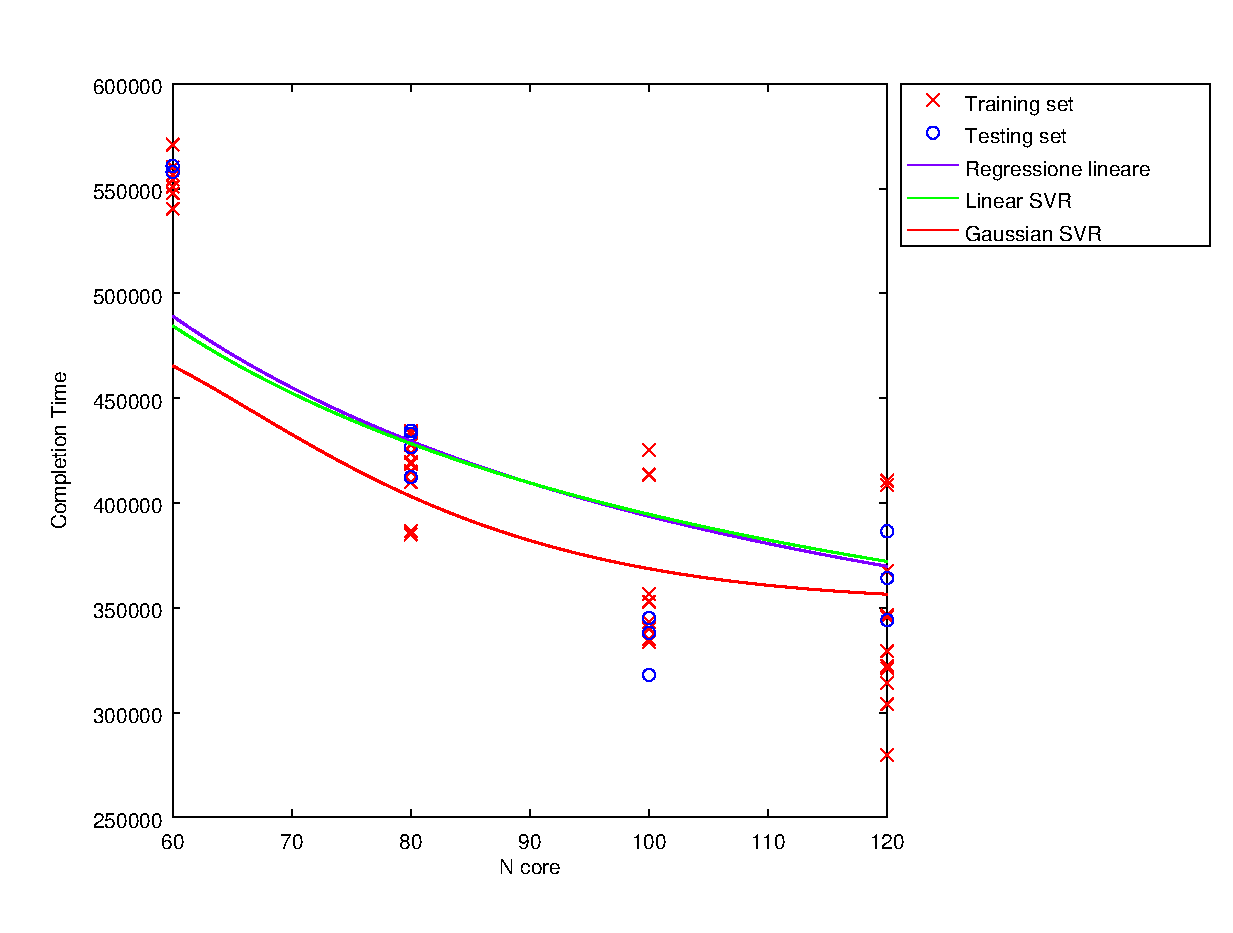
\includegraphics[width=\textwidth]{output/R1_1000_1_OVER_NCORES/plot_R1_1000_bestmodels.eps}
\caption {Completion time vs ncores for query R1 with datasize 1000}
\end {figure}

\newpage
\subsection{Query R2}
\subsubsection{Query R2 -- Datasize 250}
\begin{table}[H]
	\centering
	\begin{adjustbox}{center}
		\begin{tabular}{c | c M{1.2cm} M{2.5cm} M{2.5cm} M{1.8cm}}
			Model & RMSE & R\textsuperscript{2} & Mean absolute error & Mean relative error & Mean difference \tabularnewline
			\hline
			Linear regression & 0.3084 & 0.8429 &  83176 & 0.9116 & 0.1838 \\
			Linear SVR & 0.2402 & 0.9235 &  83030 & 0.5897 & 0.0233 \\
			Polynomial SVR (2) & 0.8800 & 0.2967 &  84417 & 35.7221 & 0.1311 \\
			Polynomial SVR (3) & 0.6423 & 0.6316 &  83765 & 6.7284 & 0.2887 \\
			Polynomial SVR (4) & 0.7945 & 0.0199 &  84228 & 21.9735 & 0.0262 \\
			Polynomial SVR (6) & 0.7333 & 0.5682 &  84141 & 13.7543 & 0.0515 \\
			Gaussian SVR & 0.3433 & 0.8108 &  83318 & 0.5836 & 0.0294 \\
		\end{tabular}
	\end{adjustbox}
	\\
	\caption{Results for R2-250 with non-linear 1/ncores feature}
	\label{table_R2_prediction_all}
\end{table}

\begin {figure}[hbtp]
\centering
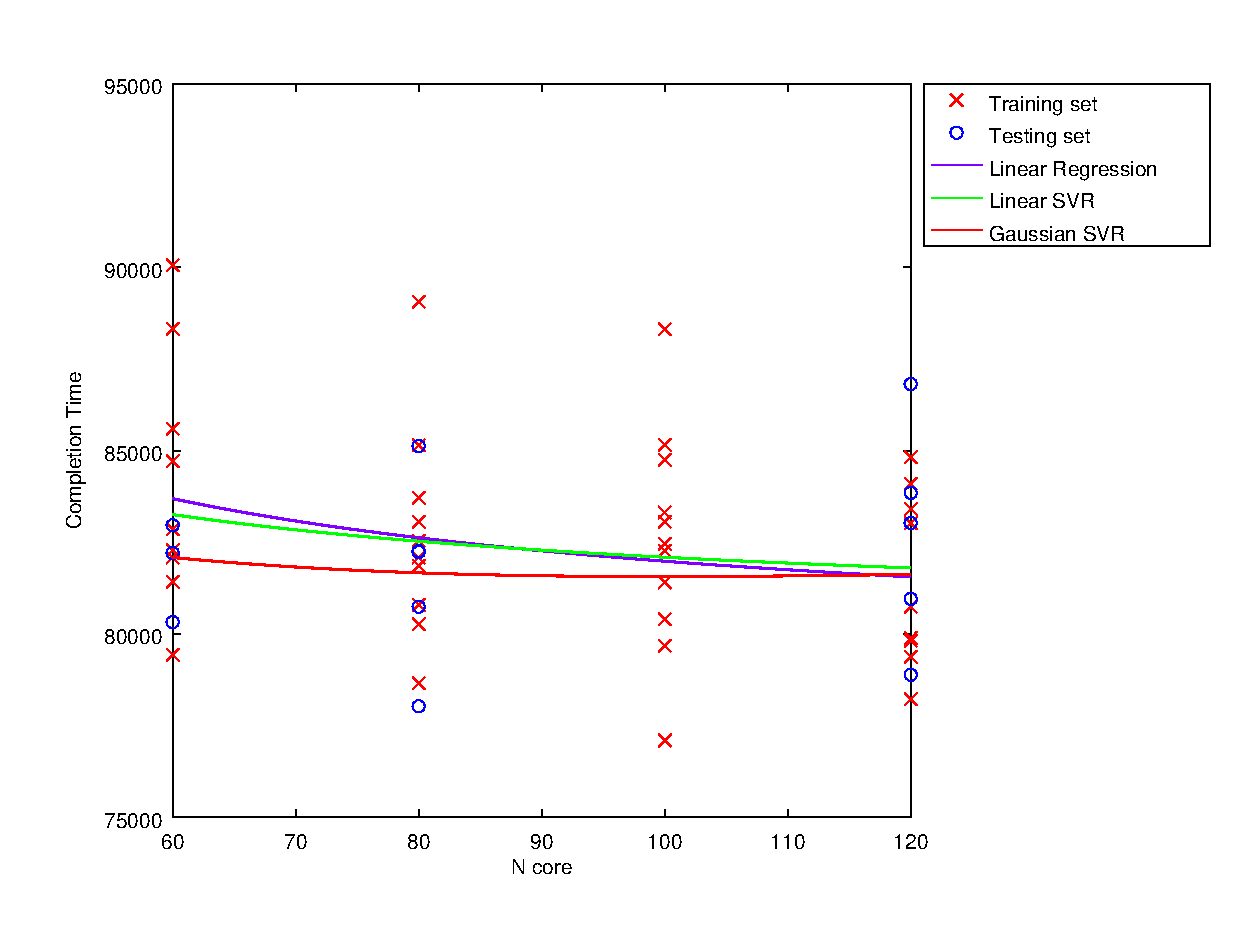
\includegraphics[width=\textwidth]{output/R2_250_NO_72_90_1_OVER_NCORES/plot_R2_250_bestmodels.eps}
\caption {Completion time vs ncores for query R2 with datasize 250}
\end {figure}

\newpage
\subsubsection{Query R2 -- Datasize 500}
\begin{table}[H]
	\centering
	\begin{adjustbox}{center}
		\begin{tabular}{c | c M{1.2cm} M{2.5cm} M{2.5cm} M{1.8cm}}
			Model & RMSE & R\textsuperscript{2} & Mean absolute error & Mean relative error & Mean difference \tabularnewline
			\hline
			Linear regression & 0.2504 & 0.9581 &  73225 & 0.5520 & -0.0447 \\
			Linear SVR & 0.2443 & 0.9617 &  73192 & 0.6815 & -0.0188 \\
			Polynomial SVR (2) & 2.2931 & 0.0395 &  76764 & 3.4868 & -0.1115 \\
			Polynomial SVR (3) & 4.3801 & 0.3401 &  78078 & 1.4172 & 1.0143 \\
			Polynomial SVR (4) & 3.2640 & 0.0185 &  78390 & 11.5499 & -0.2238 \\
			Polynomial SVR (6) & 3.4982 & 0.0292 &  77888 & 13.3950 & 0.4314 \\
			Gaussian SVR & 0.7471 & 0.7045 &  74079 & 3.0922 & -0.2571 \\
		\end{tabular}
	\end{adjustbox}
	\\
	\caption{Results for R2-500 with non-linear 1/ncores feature}
	\label{table_R2_prediction_all}
\end{table}

\begin {figure}[hbtp]
\centering
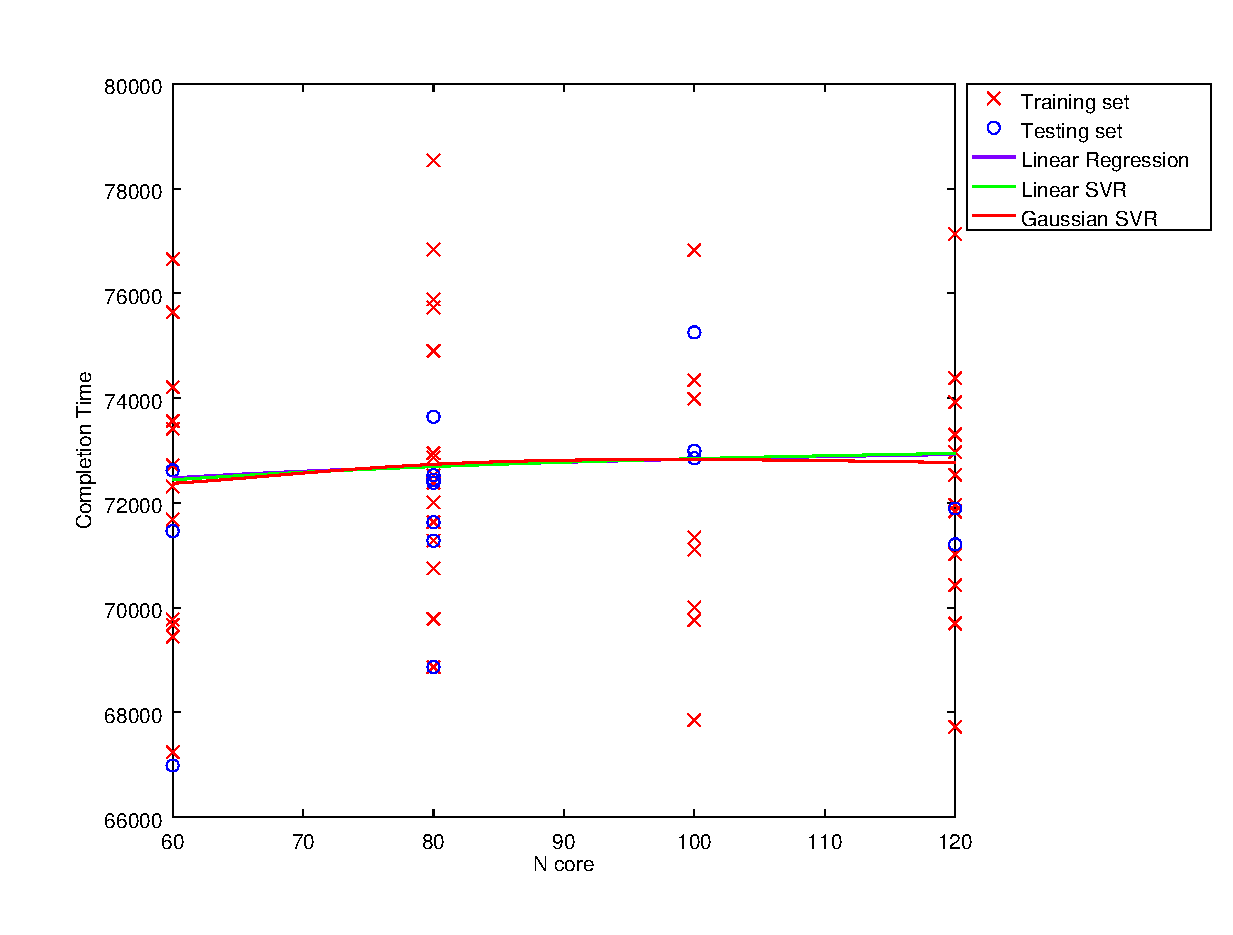
\includegraphics[width=\textwidth]{output/R2_500_1_OVER_NCORES/plot_R2_500_bestmodels.eps}
\caption {Completion time vs ncores for query R2 with datasize 500}
\end {figure}

\newpage
\subsubsection{Query R2 -- Datasize 750}
\begin{table}[H]
	\centering
	\begin{adjustbox}{center}
		\begin{tabular}{c | c M{1.2cm} M{2.5cm} M{2.5cm} M{1.8cm}}
			Model & RMSE & R\textsuperscript{2} & Mean absolute error & Mean relative error & Mean difference \tabularnewline
			\hline
			Linear regression & 0.2224 & 0.9208 &  78830 & 0.9775 & 0.0385 \\
			Linear SVR & 0.2328 & 0.9535 &  78852 & 0.9182 & -0.0008 \\
			Polynomial SVR (2) & 0.8134 & 0.2265 &  79819 & 8.6904 & -0.0437 \\
			Polynomial SVR (3) & 0.4734 & 0.6998 &  79323 & 6.8385 & 0.1398 \\
			Polynomial SVR (4) & 0.8079 & -0.0000 &  79779 & 3.1582 & -0.1683 \\
			Polynomial SVR (6) & 0.8079 & -0.0000 &  79779 & 3.1582 & -0.1683 \\
			Gaussian SVR & 0.4697 & 0.7362 &  79193 & 3.5198 & 0.1028 \\
		\end{tabular}
	\end{adjustbox}
	\\
	\caption{Results for R2-750 with non-linear 1/ncores feature}
	\label{table_R2_prediction_all}
\end{table}

\begin {figure}[hbtp]
\centering
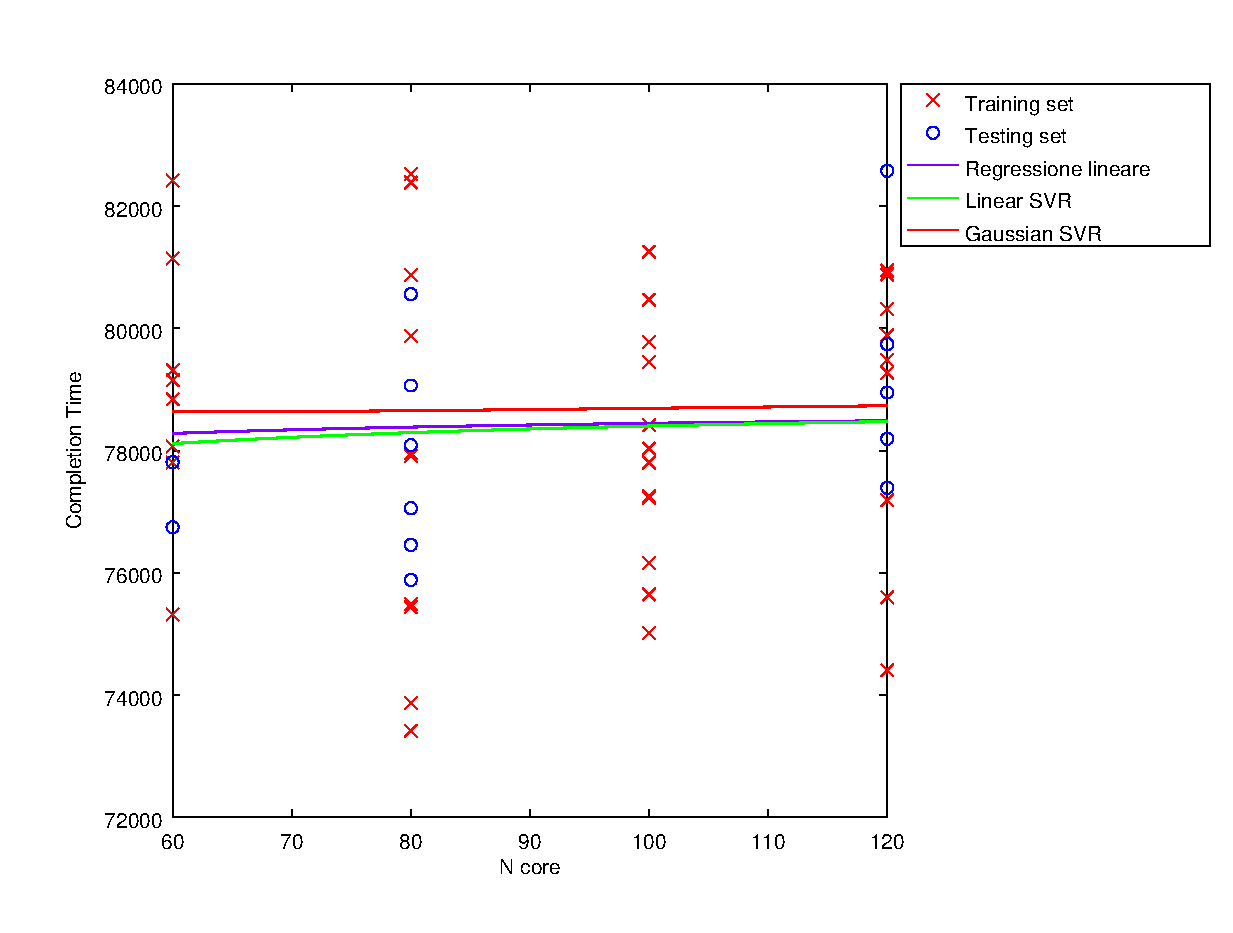
\includegraphics[width=\textwidth]{output/R2_750_1_OVER_NCORES/plot_R2_750_bestmodels.eps}
\caption {Completion time vs ncores for query R2 with datasize 750}
\end {figure}

\newpage
\subsubsection{Query R2 -- Datasize 1000}
\begin{table}[H]
	\centering
	\begin{adjustbox}{center}
		\begin{tabular}{c | c M{1.2cm} M{2.5cm} M{2.5cm} M{1.8cm}}
			Model & RMSE & R\textsuperscript{2} & Mean absolute error & Mean relative error & Mean difference \tabularnewline
			\hline
			Linear regression & 0.0462 & 0.9983 & 1124528 & 0.1815 & 0.0091 \\
			Linear SVR & 0.0822 & 0.9949 & 1140186 & 0.2180 & -0.0168 \\
			Polynomial SVR (2) & 0.7408 & 0.5722 & 1456474 & 2.1287 & 0.0114 \\
			Polynomial SVR (3) & 0.4716 & 0.9256 & 1285649 & 0.7305 & 0.2304 \\
			Polynomial SVR (4) & 0.8006 & 0.5912 & 1461556 & 5.8049 & 0.0416 \\
			Polynomial SVR (6) & 1.2837 & 0.0083 & 1575200 & 11.0978 & -0.2082 \\
			Gaussian SVR & 0.2323 & 0.9735 & 1176463 & 0.2942 & -0.0733 \\
		\end{tabular}
	\end{adjustbox}
	\\
	\caption{Results for R2-1000 with non-linear 1/ncores feature}
	\label{table_R2_prediction_all}
\end{table}

\begin {figure}[hbtp]
\centering
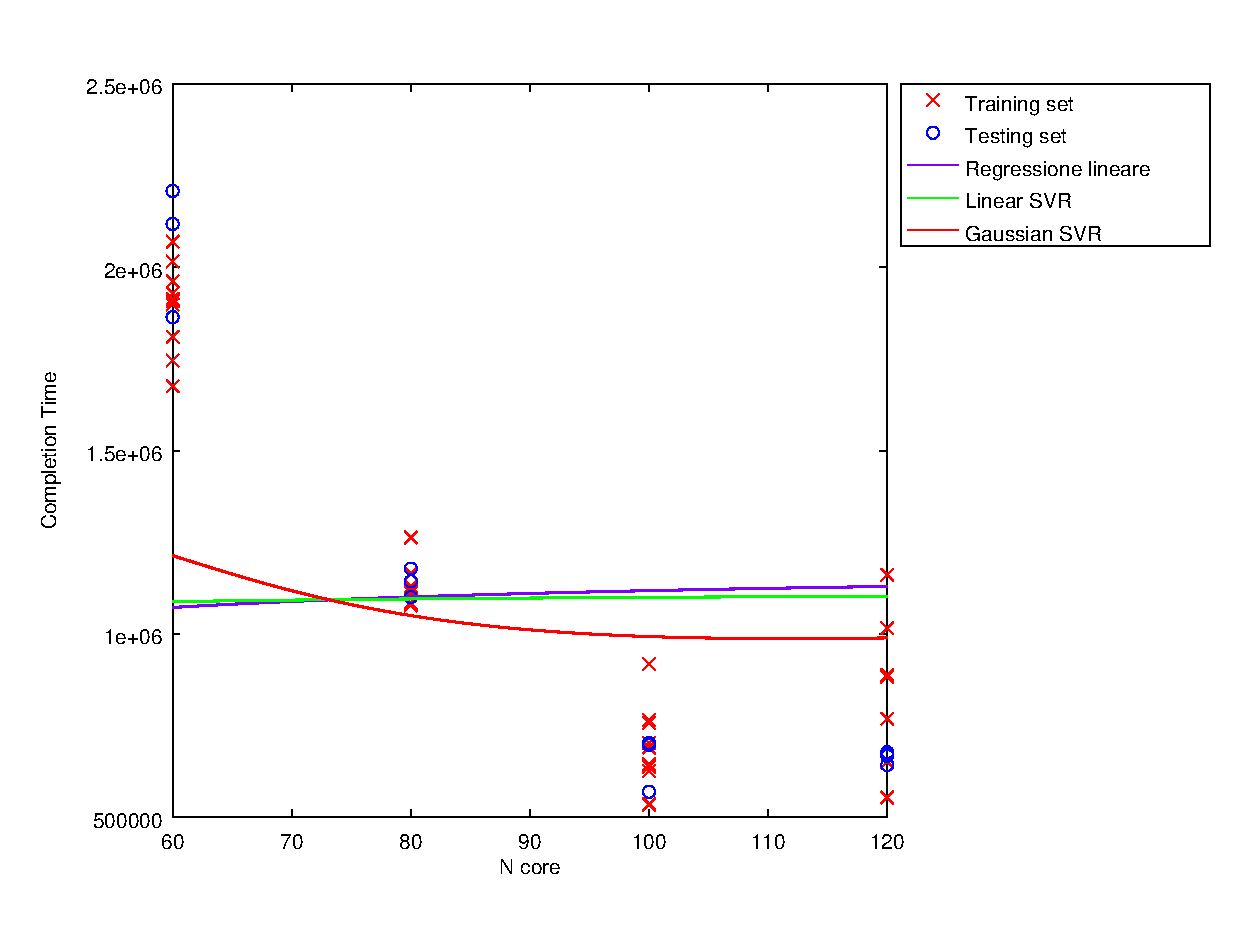
\includegraphics[width=\textwidth]{output/R2_1000_1_OVER_NCORES/plot_R2_1000_bestmodels.eps}
\caption {Completion time vs ncores for query R2 with datasize 1000}
\end {figure}

\newpage
\subsection{Query R3}
\subsubsection{Query R3 -- Datasize 250}
\begin{table}[H]
	\centering
	\begin{adjustbox}{center}
		\begin{tabular}{c | c M{1.2cm} M{2.5cm} M{2.5cm} M{1.8cm}}
			Model & RMSE & R\textsuperscript{2} & Mean absolute error & Mean relative error & Mean difference \tabularnewline
			\hline
			Linear regression & 0.1837 & 0.9536 & 188261 & 0.1659 & -0.0515 \\
			Linear SVR & 0.1351 & 0.9829 & 188650 & 1.4356 & -0.0112 \\
			Polynomial SVR (2) & 0.7236 & 0.3478 & 225546 & 7.5346 & -0.2124 \\
			Polynomial SVR (3) & 0.5047 & 0.8512 & 210478 & 2.4581 & -0.1776 \\
			Polynomial SVR (4) & 0.6953 & 0.4710 & 224755 & 3.3660 & -0.1323 \\
			Polynomial SVR (6) & 0.8553 & 0.4770 & 229792 & 4.8395 & -0.1500 \\
			Gaussian SVR & 0.3731 & 0.8522 & 197922 & 0.5825 & 0.0201 \\
		\end{tabular}
	\end{adjustbox}
	\\
	\caption{Results for R3-250 with non-linear 1/ncores feature}
	\label{table_R3_prediction_all}
\end{table}

\begin {figure}[hbtp]
\centering
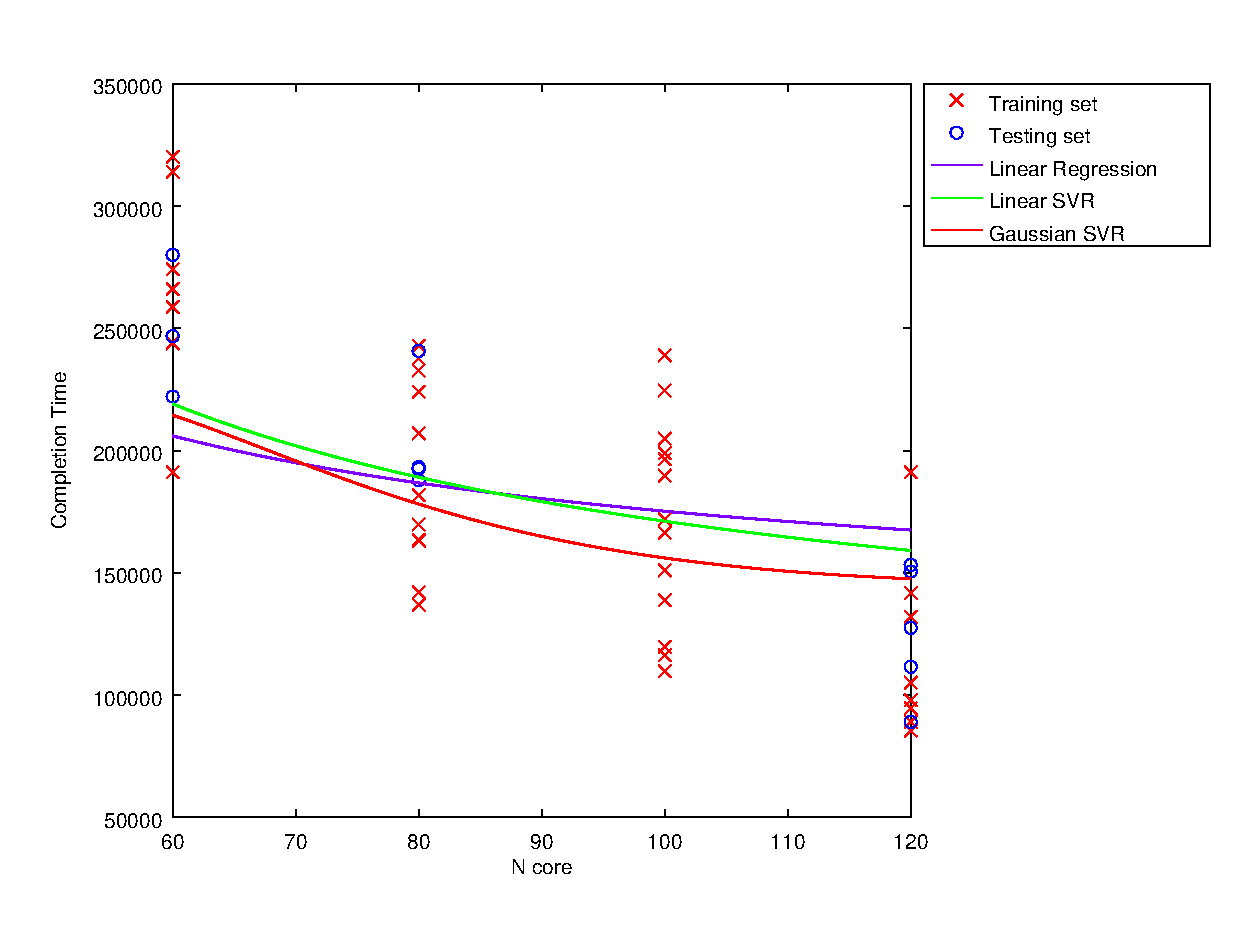
\includegraphics[width=\textwidth]{output/R3_250_NO_72_90_1_OVER_NCORES/plot_R3_250_bestmodels.eps}
\caption {Completion time vs ncores for query R3 with datasize 250}
\end {figure}

\newpage
\subsubsection{Query R3 -- Datasize 500}
\begin{table}[H]
	\centering
	\begin{adjustbox}{center}
		\begin{tabular}{c | c M{1.2cm} M{2.5cm} M{2.5cm} M{1.8cm}}
			Model & RMSE & R\textsuperscript{2} & Mean absolute error & Mean relative error & Mean difference \tabularnewline
			\hline
			Linear regression & 0.0492 & 0.9980 & 586374 & 0.0769 & -0.0179 \\
			Linear SVR & 0.0694 & 0.9979 & 592263 & 0.0844 & -0.0441 \\
			Polynomial SVR (2) & 0.4996 & 0.8693 & 683733 & 0.6110 & -0.1811 \\
			Polynomial SVR (3) & 0.2543 & 0.9661 & 637551 & 0.6338 & -0.0207 \\
			Polynomial SVR (4) & 0.4166 & 0.9154 & 665945 & 0.5385 & -0.1210 \\
			Polynomial SVR (6) & 0.5017 & 0.8823 & 680924 & 0.7386 & -0.1239 \\
			Gaussian SVR & 0.1371 & 0.9846 & 604365 & 9.4363 & -0.0214 \\
		\end{tabular}
	\end{adjustbox}
	\\
	\caption{Results for R3-500 with non-linear 1/ncores feature}
	\label{table_R3_prediction_all}
\end{table}

\begin {figure}[hbtp]
\centering
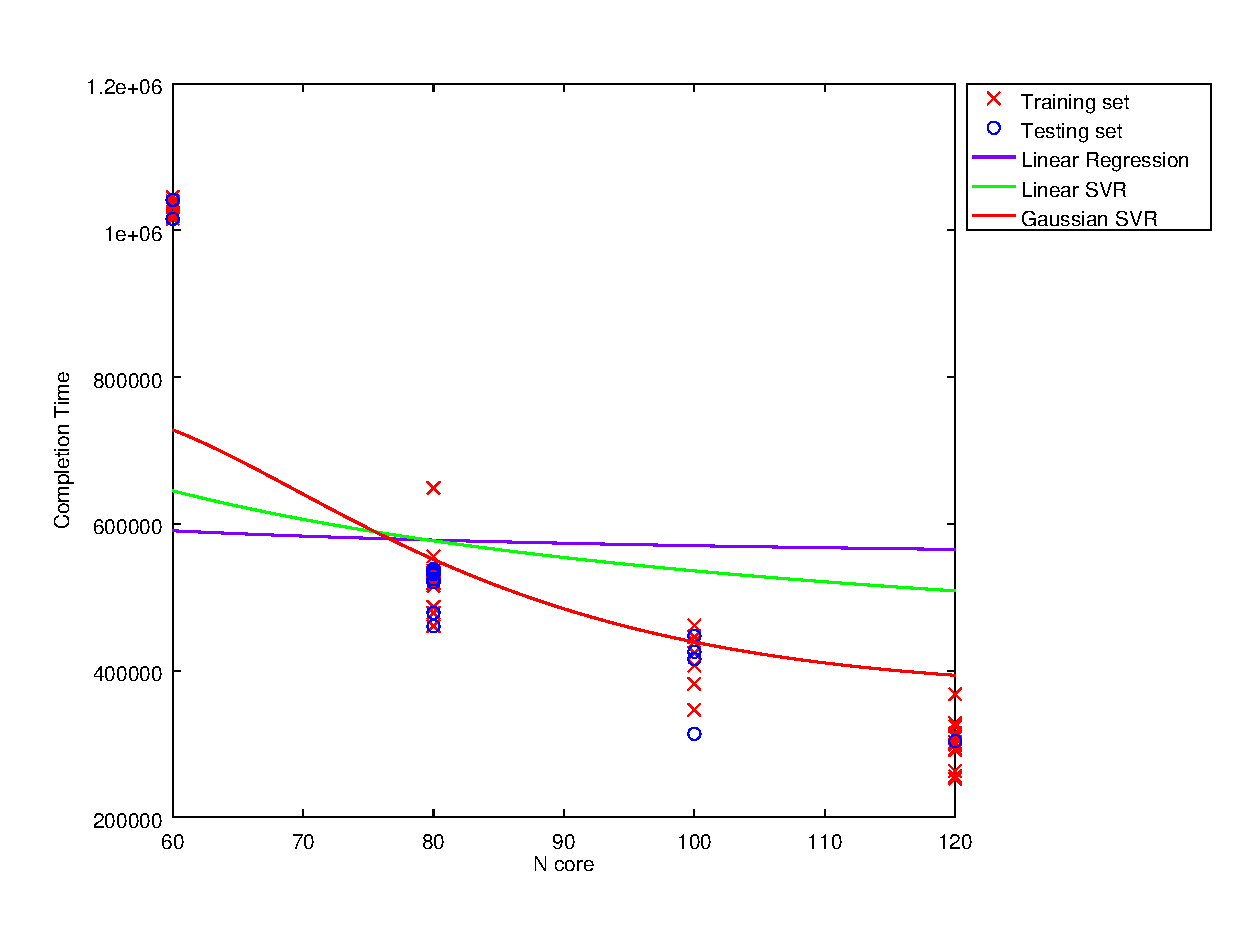
\includegraphics[width=\textwidth]{output/R3_500_1_OVER_NCORES/plot_R3_500_bestmodels.eps}
\caption {Completion time vs ncores for query R3 with datasize 500}
\end {figure}

\newpage
\subsubsection{Query R3 -- Datasize 750}
\begin{table}[H]
	\centering
	\begin{adjustbox}{center}
		\begin{tabular}{c | c M{1.2cm} M{2.5cm} M{2.5cm} M{1.8cm}}
			Model & RMSE & R\textsuperscript{2} & Mean absolute error & Mean relative error & Mean difference \tabularnewline
			\hline
			Linear regression & 0.0188 & 0.9997 & 777381 & 0.0691 & -0.0031 \\
			Linear SVR & 0.0940 & 0.9929 & 787385 & 0.2265 & 0.0245 \\
			Polynomial SVR (2) & 0.6773 & 0.5680 & 867860 & 2.0158 & -0.0217 \\
			Polynomial SVR (3) & 0.3555 & 0.9149 & 820888 & 0.9252 & 0.0371 \\
			Polynomial SVR (4) & 0.6696 & 0.6658 & 871623 & 2.3705 & 0.0400 \\
			Polynomial SVR (6) & 0.6893 & 0.6707 & 872687 & 1.9120 & -0.0459 \\
			Gaussian SVR & 0.2402 & 0.9602 & 802960 & 0.3887 & 0.1019 \\
		\end{tabular}
	\end{adjustbox}
	\\
	\caption{Results for R3-750 with non-linear 1/ncores feature}
	\label{table_R3_prediction_all}
\end{table}

\begin {figure}[hbtp]
\centering
\includegraphics[width=\textwidth]{output/R3_750_1_OVER_NCORES/plot_R3_750_bestmodels.eps}
\caption {Completion time vs ncores for query R3 with datasize 750}
\end {figure}

\newpage
\subsubsection{Query R3 -- Datasize 1000}
\begin{table}[H]
	\centering
	\begin{adjustbox}{center}
		\begin{tabular}{c | c M{1.2cm} M{2.5cm} M{2.5cm} M{1.8cm}}
			Model & RMSE & R\textsuperscript{2} & Mean absolute error & Mean relative error & Mean difference \tabularnewline
			\hline
			Linear regression & 0.0982 & 0.9905 & 1030253 & 0.4656 & -0.0388 \\
			Linear SVR & 0.1197 & 0.9920 & 1041486 & 0.4661 & -0.0713 \\
			Polynomial SVR (2) & 0.8322 & 0.3184 & 1192377 & 5.5161 & -0.0309 \\
			Polynomial SVR (3) & 0.3814 & 0.8902 & 1076692 & 0.5328 & -0.0773 \\
			Polynomial SVR (4) & 0.9713 & 0.0859 & 1199980 & 3.3847 & -0.1187 \\
			Polynomial SVR (6) & 0.7545 & 0.6282 & 1164586 & 6.4512 & -0.1462 \\
			Gaussian SVR & 0.3937 & 0.8968 & 1085557 & 1.8102 & -0.0157 \\
		\end{tabular}
	\end{adjustbox}
	\\
	\caption{Results for R3-1000 with non-linear 1/ncores feature}
	\label{table_R3_prediction_all}
\end{table}

\begin {figure}[hbtp]
\centering
\includegraphics[width=\textwidth]{output/R3_1000_1_OVER_NCORES/plot_R3_1000_bestmodels.eps}
\caption {Completion time vs ncores for query R3 with datasize 1000}
\end {figure}

\newpage
\subsection{Query R4}
\subsubsection{Query R4 -- Datasize 250}
\begin{table}[H]
	\centering
	\begin{adjustbox}{center}
		\begin{tabular}{c | c M{1.2cm} M{2.5cm} M{2.5cm} M{1.8cm}}
			Model & RMSE & R\textsuperscript{2} & Mean absolute error & Mean relative error & Mean difference \tabularnewline
			\hline
			Linear regression & 0.0844 & 0.9923 & 144609 & 0.1360 & 0.0280 \\
			Linear SVR & 0.1151 & 0.9898 & 145968 & 0.2666 & 0.0488 \\
			Polynomial SVR (2) & 0.6884 & 0.4993 & 169863 & 1.7471 & 0.0032 \\
			Polynomial SVR (3) & 0.3741 & 0.8762 & 155294 & 0.5718 & -0.0005 \\
			Polynomial SVR (4) & 0.7028 & 0.4946 & 167225 & 6.1995 & -0.1481 \\
			Polynomial SVR (6) & 0.8019 & 0.4416 & 173122 & 6.2652 & -0.1848 \\
			Gaussian SVR & 0.1906 & 0.9723 & 148942 & 2.0154 & -0.0117 \\
		\end{tabular}
	\end{adjustbox}
	\\
	\caption{Results for R4-250 with non-linear 1/ncores feature}
	\label{table_R4_prediction_all}
\end{table}

\begin {figure}[hbtp]
\centering
\includegraphics[width=\textwidth]{output/R4_250_NO_72_90_1_OVER_NCORES/plot_R4_250_bestmodels.eps}
\caption {Completion time vs ncores for query R4 with datasize 250}
\end {figure}

\newpage
\subsubsection{Query R4 -- Datasize 500}
\begin{table}[H]
	\centering
	\begin{adjustbox}{center}
		\begin{tabular}{c | c M{1.2cm} M{2.5cm} M{2.5cm} M{1.8cm}}
			Model & RMSE & R\textsuperscript{2} & Mean absolute error & Mean relative error & Mean difference \tabularnewline
			\hline
			Linear regression & 0.1039 & 0.9899 & 461984 & 0.0853 & -0.0575 \\
			Linear SVR & 0.1437 & 0.9863 & 469854 & 0.1652 & -0.0741 \\
			Polynomial SVR (2) & 0.7181 & 0.5918 & 554632 & 1.8115 & 0.2603 \\
			Polynomial SVR (3) & 0.1830 & 0.9713 & 471892 & 0.1837 & -0.0402 \\
			Polynomial SVR (4) & 0.4879 & 0.8301 & 513705 & 3.3636 & 0.2170 \\
			Polynomial SVR (6) & 0.3941 & 0.8979 & 504258 & 0.9466 & 0.1937 \\
			Gaussian SVR & 0.1715 & 0.9822 & 470231 & 0.4231 & 0.0912 \\
		\end{tabular}
	\end{adjustbox}
	\\
	\caption{Results for R4-500 with non-linear 1/ncores feature}
	\label{table_R4_prediction_all}
\end{table}

\begin {figure}[hbtp]
\centering
\includegraphics[width=\textwidth]{output/R4_500_1_OVER_NCORES/plot_R4_500_bestmodels.eps}
\caption {Completion time vs ncores for query R4 with datasize 500}
\end {figure}

\newpage
\subsubsection{Query R4 -- Datasize 750}
\begin{table}[H]
	\centering
	\begin{adjustbox}{center}
		\begin{tabular}{c | c M{1.2cm} M{2.5cm} M{2.5cm} M{1.8cm}}
			Model & RMSE & R\textsuperscript{2} & Mean absolute error & Mean relative error & Mean difference \tabularnewline
			\hline
			Linear regression & 0.0249 & 0.9993 & 609688 & 0.0767 & -0.0096 \\
			Linear SVR & 0.0775 & 0.9941 & 616317 & 0.1494 & -0.0111 \\
			Polynomial SVR (2) & 0.6998 & 0.4366 & 691144 & 2.6142 & 0.0270 \\
			Polynomial SVR (3) & 0.4296 & 0.8680 & 656260 & 0.8650 & 0.0495 \\
			Polynomial SVR (4) & 0.7424 & 0.6278 & 691474 & 3.0453 & 0.0242 \\
			Polynomial SVR (6) & 0.7619 & 0.5988 & 692973 & 41.6362 & 0.0564 \\
			Gaussian SVR & 0.2495 & 0.9515 & 631230 & 0.5094 & 0.0416 \\
		\end{tabular}
	\end{adjustbox}
	\\
	\caption{Results for R4-750 with non-linear 1/ncores feature}
	\label{table_R4_prediction_all}
\end{table}

\begin {figure}[hbtp]
\centering
\includegraphics[width=\textwidth]{output/R4_750_1_OVER_NCORES/plot_R4_750_bestmodels.eps}
\caption {Completion time vs ncores for query R4 with datasize 750}
\end {figure}

\newpage
\subsubsection{Query R4 -- Datasize 1000}
\begin{table}[H]
	\centering
	\begin{adjustbox}{center}
		\begin{tabular}{c | c M{1.2cm} M{2.5cm} M{2.5cm} M{1.8cm}}
			Model & RMSE & R\textsuperscript{2} & Mean absolute error & Mean relative error & Mean difference \tabularnewline
			\hline
			Linear regression & 0.1178 & 0.9858 & 1780763 & 0.3091 & -0.0268 \\
			Linear SVR & 0.1508 & 0.9781 & 1815061 & 0.3434 & -0.0358 \\
			Polynomial SVR (2) & 0.6123 & 0.6395 & 2147223 & 8.6372 & 0.1279 \\
			Polynomial SVR (3) & 0.8708 & 0.6596 & 2194020 & 1.7499 & 0.1679 \\
			Polynomial SVR (4) & 1.4316 & 0.5428 & 2389075 & 8.5766 & 0.3266 \\
			Polynomial SVR (6) & 2.2003 & 0.4893 & 2612105 & 2.9349 & 0.4842 \\
			Gaussian SVR & 0.3502 & 0.8931 & 1871949 & 0.3178 & -0.1009 \\
		\end{tabular}
	\end{adjustbox}
	\\
	\caption{Results for R4-1000 with non-linear 1/ncores feature}
	\label{table_R4_prediction_all}
\end{table}

\begin {figure}[hbtp]
\centering
\includegraphics[width=\textwidth]{output/R4_1000_1_OVER_NCORES/plot_R4_1000_bestmodels.eps}
\caption {Completion time vs ncores for query R4 with datasize 1000}
\end {figure}

\newpage
\subsection{Query R5}
\subsubsection{Query R5 -- Datasize 250}
\begin{table}[H]
	\centering
	\begin{adjustbox}{center}
		\begin{tabular}{c | c M{1.2cm} M{2.5cm} M{2.5cm} M{1.8cm}}
			Model & RMSE & R\textsuperscript{2} & Mean absolute error & Mean relative error & Mean difference \tabularnewline
			\hline
			Linear regression & 0.7902 & 0.4355 &  25692 & 1.3583 & 0.0245 \\
			Linear SVR & 0.8017 & 0.4899 &  25695 & 11.0402 & 0.0640 \\
			Polynomial SVR (2) & 1.0464 & 0.0532 &  25915 & 12.6721 & 0.2061 \\
			Polynomial SVR (3) & 1.1437 & 0.0000 &  26070 & 3.6631 & 0.4490 \\
			Polynomial SVR (4) & 1.1437 & 0.0000 &  26070 & 3.6631 & 0.4490 \\
			Polynomial SVR (6) & 1.1437 & 0.0000 &  26070 & 3.6631 & 0.4490 \\
			Gaussian SVR & 0.7178 & 0.5705 &  25673 & 0.9514 & -0.0608 \\
		\end{tabular}
	\end{adjustbox}
	\\
	\caption{Results for R5-250 with non-linear 1/ncores feature}
	\label{table_R5_prediction_all}
\end{table}

\begin {figure}[hbtp]
\centering
\includegraphics[width=\textwidth]{output/R5_250_NO_72_90_1_OVER_NCORES/plot_R5_250_bestmodels.eps}
\caption {Completion time vs ncores for query R5 with datasize 250}
\end {figure}

\newpage
\subsubsection{Query R5 -- Datasize 500}
\begin{table}[H]
	\centering
	\begin{adjustbox}{center}
		\begin{tabular}{c | c M{1.2cm} M{2.5cm} M{2.5cm} M{1.8cm}}
			Model & RMSE & R\textsuperscript{2} & Mean absolute error & Mean relative error & Mean difference \tabularnewline
			\hline
			Linear regression & 0.2378 & 0.9442 &  23771 & 0.2128 & -0.0053 \\
			Linear SVR & 0.1676 & 0.9751 &  23712 & 0.1419 & -0.0466 \\
			Polynomial SVR (2) & 0.7513 & 0.7351 &  24396 & 6.0060 & 0.1990 \\
			Polynomial SVR (3) & 0.5981 & 0.7171 &  23987 & 0.4265 & -0.0989 \\
			Polynomial SVR (4) & 0.9651 & 0.1515 &  24696 & 10.4681 & 0.1982 \\
			Polynomial SVR (6) & 1.0094 & 0.0276 &  24731 & 9.3838 & 0.1498 \\
			Gaussian SVR & 0.2083 & 0.9598 &  23753 & 0.2258 & -0.0203 \\
		\end{tabular}
	\end{adjustbox}
	\\
	\caption{Results for R5-500 with non-linear 1/ncores feature}
	\label{table_R5_prediction_all}
\end{table}

\begin {figure}[hbtp]
\centering
\includegraphics[width=\textwidth]{output/R5_500_1_OVER_NCORES/plot_R5_500_bestmodels.eps}
\caption {Completion time vs ncores for query R5 with datasize 500}
\end {figure}

\newpage
\subsubsection{Query R5 -- Datasize 750}
\begin{table}[H]
	\centering
	\begin{adjustbox}{center}
		\begin{tabular}{c | c M{1.2cm} M{2.5cm} M{2.5cm} M{1.8cm}}
			Model & RMSE & R\textsuperscript{2} & Mean absolute error & Mean relative error & Mean difference \tabularnewline
			\hline
			Linear regression & 1.2329 & -0.5849 &  24805 & 0.9817 & -0.2918 \\
			Linear SVR & 1.1139 & 0.0150 &  24796 & 1.9259 & -0.2447 \\
			Polynomial SVR (2) & 1.0313 & 0.0125 &  25012 & 4.8103 & -0.3399 \\
			Polynomial SVR (3) & 1.1771 & 0.0537 &  24878 & 1.9265 & -0.3482 \\
			Polynomial SVR (4) & 1.0605 & 0.0354 &  25042 & 14.9151 & -0.3808 \\
			Polynomial SVR (6) & 1.0680 & 0.0681 &  25049 & 9.3339 & -0.4060 \\
			Gaussian SVR & 1.0073 & 0.1519 &  24632 & 0.7970 & -0.3309 \\
		\end{tabular}
	\end{adjustbox}
	\\
	\caption{Results for R5-750 with non-linear 1/ncores feature}
	\label{table_R5_prediction_all}
\end{table}

\begin {figure}[hbtp]
\centering
\includegraphics[width=\textwidth]{output/R5_750_1_OVER_NCORES/plot_R5_750_bestmodels.eps}
\caption {Completion time vs ncores for query R5 with datasize 750}
\end {figure}

\newpage
\subsubsection{Query R5 -- Datasize 1000}
\begin{table}[H]
	\centering
	\begin{adjustbox}{center}
		\begin{tabular}{c | c M{1.2cm} M{2.5cm} M{2.5cm} M{1.8cm}}
			Model & RMSE & R\textsuperscript{2} & Mean absolute error & Mean relative error & Mean difference \tabularnewline
			\hline
			Linear regression & 0.7757 & 0.1272 &  40269 & 8.1325 & 0.1327 \\
			Linear SVR & 0.4719 & 0.6897 &  39564 & 1.1892 & -0.0627 \\
			Polynomial SVR (2) & 0.5218 & 0.8335 &  39510 & 0.5824 & 0.1911 \\
			Polynomial SVR (3) & 0.4815 & 0.7456 &  39434 & 0.7028 & -0.1583 \\
			Polynomial SVR (4) & 2.1891 & 0.6549 &  41612 & 0.8490 & 0.7659 \\
			Polynomial SVR (6) & 9.0686 & 0.5421 &  49794 & 0.8052 & 3.0575 \\
			Gaussian SVR & 0.3401 & 0.8418 &  39083 & 0.6944 & 0.0572 \\
		\end{tabular}
	\end{adjustbox}
	\\
	\caption{Results for R5-1000 with non-linear 1/ncores feature}
	\label{table_R5_prediction_all}
\end{table}

\begin {figure}[hbtp]
\centering
\includegraphics[width=\textwidth]{output/R5_1000_1_OVER_NCORES/plot_R5_1000_bestmodels.eps}
\caption {Completion time vs ncores for query R5 with datasize 1000}
\end {figure}

%--------------------------------------------

\newpage
\section{Fixed Datasize, $ncores^{-1}$, Only $ncores$}
\subsection{Query R1}
\subsubsection{Query R1 -- Datasize 250}
\begin{table}[H]
	\centering
	\begin{adjustbox}{center}
		\begin{tabular}{c | c M{1.2cm} M{2.5cm} M{2.5cm} M{1.8cm}}
			Model & RMSE & R\textsuperscript{2} & Mean absolute error & Mean relative error & Mean difference \tabularnewline
			\hline
			Linear regression & 1.2438 & 0.3259 &  69940 & 4.1591 & -0.3070 \\
			Linear SVR & 1.2946 & 0.3792 &  69617 & 9.8952 & -0.4115 \\
			Polynomial SVR (2) & 1.5679 & 0.0009 &  78957 & 23.3735 & -0.2765 \\
			Polynomial SVR (3) & 1.3800 & 0.2700 &  71046 & 1.6291 & -0.4540 \\
			Polynomial SVR (4) & 1.5428 & 0.0283 &  77216 & 3.2523 & -0.3834 \\
			Polynomial SVR (6) & 1.4977 & 0.0704 &  75624 & 2.2494 & -0.3222 \\
			Gaussian SVR & 1.2913 & 0.4092 &  69556 & 69.7144 & -0.4357 \\
		\end{tabular}
	\end{adjustbox}
	\\
	\caption{Results for R1-250 considering only non-linear 1/ncores feature}
	\label{table_R1_prediction_all}
\end{table}

\begin {figure}[hbtp]
\centering
\includegraphics[width=\textwidth]{output/R1_250_ONLY_1_OVER_NCORES/plot_R1_250_bestmodels.eps}
\caption {Completion time vs ncores for query R1 with datasize 250 with only 1/ncores feature}
\end {figure}

\newpage
\subsubsection{Query R1 -- Datasize 500}
\begin{table}[H]
	\centering
	\begin{adjustbox}{center}
		\begin{tabular}{c | c M{1.2cm} M{2.5cm} M{2.5cm} M{1.8cm}}
			Model & RMSE & R\textsuperscript{2} & Mean absolute error & Mean relative error & Mean difference \tabularnewline
			\hline
			Linear regression & 0.4299 & -0.8239 & 186098 & 1.0456 & 0.1101 \\
			Linear SVR & 0.4844 & 0.3583 & 190687 & 0.9645 & 0.1330 \\
			Polynomial SVR (2) & 0.5830 & 0.3046 & 191181 & 1.0484 & 0.1404 \\
			Polynomial SVR (3) & 0.2854 & 0.2958 & 174622 & 1.1754 & 0.0854 \\
			Polynomial SVR (4) & 0.4208 & 0.2616 & 183858 & 9.0979 & 0.0165 \\
			Polynomial SVR (6) & 0.3558 & 0.2475 & 180322 & 0.9703 & 0.0168 \\
			Gaussian SVR & 0.2599 & 0.3430 & 174651 & 0.8709 & 0.0205 \\
		\end{tabular}
	\end{adjustbox}
	\\
	\caption{Results for R1-500 considering only non-linear 1/ncores feature}
	\label{table_R1_prediction_all}
\end{table}

\begin {figure}[hbtp]
\centering
\includegraphics[width=\textwidth]{output/R1_500_ONLY_1_OVER_NCORES/plot_R1_500_bestmodels.eps}
\caption {Completion time vs ncores for query R1 with datasize 500 with only 1/ncores feature}
\end {figure}

\newpage
\subsubsection{Query R1 -- Datasize 750}
\begin{table}[H]
	\centering
	\begin{adjustbox}{center}
		\begin{tabular}{c | c M{1.2cm} M{2.5cm} M{2.5cm} M{1.8cm}}
			Model & RMSE & R\textsuperscript{2} & Mean absolute error & Mean relative error & Mean difference \tabularnewline
			\hline
			Linear regression & 0.5196 & 0.3983 & 301071 & 1.4325 & 0.0161 \\
			Linear SVR & 0.5593 & 0.4060 & 301291 & 1.0648 & 0.2096 \\
			Polynomial SVR (2) & 0.9889 & 0.3005 & 335427 & 2.5686 & 0.2086 \\
			Polynomial SVR (3) & 0.5764 & 0.2683 & 303740 & 1.3759 & -0.0300 \\
			Polynomial SVR (4) & 0.8258 & 0.2413 & 321119 & 2.7541 & 0.0410 \\
			Polynomial SVR (6) & 0.7387 & 0.2238 & 313524 & 1.3009 & -0.0036 \\
			Gaussian SVR & 0.5548 & 0.4014 & 304893 & 1.6951 & 0.1742 \\
		\end{tabular}
	\end{adjustbox}
	\\
	\caption{Results for R1-750 considering only non-linear 1/ncores feature}
	\label{table_R1_prediction_all}
\end{table}

\begin {figure}[hbtp]
\centering
\includegraphics[width=\textwidth]{output/R1_750_ONLY_1_OVER_NCORES/plot_R1_750_bestmodels.eps}
\caption {Completion time vs ncores for query R1 with datasize 750 with only 1/ncores feature}
\end {figure}

\newpage
\subsubsection{Query R1 -- Datasize 1000}
\begin{table}[H]
	\centering
	\begin{adjustbox}{center}
		\begin{tabular}{c | c M{1.2cm} M{2.5cm} M{2.5cm} M{1.8cm}}
			Model & RMSE & R\textsuperscript{2} & Mean absolute error & Mean relative error & Mean difference \tabularnewline
			\hline
			Linear regression & 0.4522 & 0.8354 & 452627 & 0.6956 & 0.0466 \\
			Linear SVR & 0.4523 & 0.8418 & 452924 & 0.7178 & 0.0256 \\
			Polynomial SVR (2) & 0.9219 & 0.3472 & 503186 & 60.6930 & -0.1777 \\
			Polynomial SVR (3) & 0.5579 & 0.7553 & 461962 & 0.8781 & -0.0831 \\
			Polynomial SVR (4) & 0.7691 & 0.5531 & 486863 & 2.6097 & -0.0537 \\
			Polynomial SVR (6) & 0.6837 & 0.6343 & 471450 & 1.6197 & 0.1147 \\
			Gaussian SVR & 0.4025 & 0.8860 & 447518 & 4.2138 & 0.0524 \\
		\end{tabular}
	\end{adjustbox}
	\\
	\caption{Results for R1-1000 considering only non-linear 1/ncores feature}
	\label{table_R1_prediction_all}
\end{table}

\begin {figure}[hbtp]
\centering
\includegraphics[width=\textwidth]{output/R1_1000_ONLY_1_OVER_NCORES/plot_R1_1000_bestmodels.eps}
\caption {Completion time vs ncores for query R1 with datasize 1000 with only 1/ncores feature}
\end {figure}

\newpage
\subsection{Query R2}
\subsubsection{Query R2 -- Datasize 250}
\begin{table}[H]
	\centering
	\begin{adjustbox}{center}
		\begin{tabular}{c | c M{1.2cm} M{2.5cm} M{2.5cm} M{1.8cm}}
			Model & RMSE & R\textsuperscript{2} & Mean absolute error & Mean relative error & Mean difference \tabularnewline
			\hline
			Linear regression & 1.1144 & -0.1605 &  86606 & 43.9004 & 0.5333 \\
			Linear SVR & 1.0999 & 0.3336 &  86535 & 12.2781 & 0.4984 \\
			Polynomial SVR (2) & 1.2137 & 0.2301 &  86821 & 97.7931 & 0.5667 \\
			Polynomial SVR (3) & 1.1385 & 0.1887 &  86639 & 24.1856 & 0.5212 \\
			Polynomial SVR (4) & 1.2061 & 0.1636 &  86830 & 55.5557 & 0.5837 \\
			Polynomial SVR (6) & 1.1742 & 0.1449 &  86666 & 21.9217 & 0.5206 \\
			Gaussian SVR & 1.1479 & 0.3465 &  86748 & 19.8558 & 0.6024 \\
		\end{tabular}
	\end{adjustbox}
	\\
	\caption{Results for R2-250 considering only non-linear 1/ncores feature}
	\label{table_R2_prediction_all}
\end{table}

\begin {figure}[hbtp]
\centering
\includegraphics[width=\textwidth]{output/R2_250_ONLY_1_OVER_NCORES/plot_R2_250_bestmodels.eps}
\caption {Completion time vs ncores for query R2 with datasize 250 with only 1/ncores feature}
\end {figure}

\newpage
\subsubsection{Query R2 -- Datasize 500}
\begin{table}[H]
	\centering
	\begin{adjustbox}{center}
		\begin{tabular}{c | c M{1.2cm} M{2.5cm} M{2.5cm} M{1.8cm}}
			Model & RMSE & R\textsuperscript{2} & Mean absolute error & Mean relative error & Mean difference \tabularnewline
			\hline
			Linear regression & 0.8450 & -0.0683 &  74946 & 1942.7439 & 0.2036 \\
			Linear SVR & 0.9098 & 0.0000 &  75155 & 3.9493 & 0.3992 \\
			Polynomial SVR (2) & 0.8688 & 0.0695 &  74985 & 9.5569 & 0.3579 \\
			Polynomial SVR (3) & 0.9098 & 0.0000 &  75155 & 3.9493 & 0.3992 \\
			Polynomial SVR (4) & 0.8660 & 0.0737 &  74979 & 9.4332 & 0.3510 \\
			Polynomial SVR (6) & 0.8683 & 0.0677 &  74987 & 9.3695 & 0.3529 \\
			Gaussian SVR & 0.9098 & 0.0000 &  75155 & 3.9493 & 0.3992 \\
		\end{tabular}
	\end{adjustbox}
	\\
	\caption{Results for R2-500 considering only non-linear 1/ncores feature}
	\label{table_R2_prediction_all}
\end{table}

\begin {figure}[hbtp]
\centering
\includegraphics[width=\textwidth]{output/R2_500_ONLY_1_OVER_NCORES/plot_R2_500_bestmodels.eps}
\caption {Completion time vs ncores for query R2 with datasize 500 with only 1/ncores feature}
\end {figure}

\newpage
\subsubsection{Query R2 -- Datasize 750}
\begin{table}[H]
	\centering
	\begin{adjustbox}{center}
		\begin{tabular}{c | c M{1.2cm} M{2.5cm} M{2.5cm} M{1.8cm}}
			Model & RMSE & R\textsuperscript{2} & Mean absolute error & Mean relative error & Mean difference \tabularnewline
			\hline
			Linear regression & 1.1428 & -0.7782 &  80571 & 11.0018 & -0.7311 \\
			Linear SVR & 1.2154 & 0.0007 &  80760 & 26.8595 & -0.8498 \\
			Polynomial SVR (2) & 1.1469 & 0.0007 &  80643 & 4.9567 & -0.7332 \\
			Polynomial SVR (3) & 1.1451 & 0.0029 &  80582 & 3.8699 & -0.7405 \\
			Polynomial SVR (4) & 1.1733 & 0.0010 &  80703 & 3.2972 & -0.7625 \\
			Polynomial SVR (6) & 1.1884 & 0.0015 &  80732 & 3.0496 & -0.7841 \\
			Gaussian SVR & 1.1685 & 0.0000 &  80656 & 5.5732 & -0.7944 \\
		\end{tabular}
	\end{adjustbox}
	\\
	\caption{Results for R2-750 considering only non-linear 1/ncores feature}
	\label{table_R2_prediction_all}
\end{table}

\begin {figure}[hbtp]
\centering
\includegraphics[width=\textwidth]{output/R2_750_ONLY_1_OVER_NCORES/plot_R2_750_bestmodels.eps}
\caption {Completion time vs ncores for query R2 with datasize 750 with only 1/ncores feature}
\end {figure}

\newpage
\subsubsection{Query R2 -- Datasize 1000}
\begin{table}[H]
	\centering
	\begin{adjustbox}{center}
		\begin{tabular}{c | c M{1.2cm} M{2.5cm} M{2.5cm} M{1.8cm}}
			Model & RMSE & R\textsuperscript{2} & Mean absolute error & Mean relative error & Mean difference \tabularnewline
			\hline
			Linear regression & 0.3620 & 0.8906 & 1283627 & 0.4741 & -0.0685 \\
			Linear SVR & 0.3947 & 0.8955 & 1286697 & 0.5284 & -0.0674 \\
			Polynomial SVR (2) & 0.7818 & 0.5184 & 1500648 & 3.3328 & -0.1846 \\
			Polynomial SVR (3) & 0.3903 & 0.8815 & 1294867 & 0.6766 & -0.0936 \\
			Polynomial SVR (4) & 0.5745 & 0.7255 & 1394095 & 1.8798 & -0.0267 \\
			Polynomial SVR (6) & 0.4923 & 0.7987 & 1355406 & 0.7814 & -0.0340 \\
			Gaussian SVR & 0.2777 & 0.9490 & 1241305 & 1.1338 & 0.0117 \\
		\end{tabular}
	\end{adjustbox}
	\\
	\caption{Results for R2-1000 considering only non-linear 1/ncores feature}
	\label{table_R2_prediction_all}
\end{table}

\begin {figure}[hbtp]
\centering
\includegraphics[width=\textwidth]{output/R2_1000_ONLY_1_OVER_NCORES/plot_R2_1000_bestmodels.eps}
\caption {Completion time vs ncores for query R2 with datasize 1000 with only 1/ncores feature}
\end {figure}

\newpage
\subsection{Query R3}
\subsubsection{Query R3 -- Datasize 250}
\begin{table}[H]
	\centering
	\begin{adjustbox}{center}
		\begin{tabular}{c | c M{1.2cm} M{2.5cm} M{2.5cm} M{1.8cm}}
			Model & RMSE & R\textsuperscript{2} & Mean absolute error & Mean relative error & Mean difference \tabularnewline
			\hline
			Linear regression & 0.6073 & 0.6555 & 220156 & 1.1869 & -0.1188 \\
			Linear SVR & 0.6177 & 0.6687 & 220214 & 1.2979 & -0.1555 \\
			Polynomial SVR (2) & 0.9097 & 0.2319 & 238176 & 29.0584 & 0.0010 \\
			Polynomial SVR (3) & 0.6375 & 0.6375 & 222035 & 1.0650 & -0.1254 \\
			Polynomial SVR (4) & 0.7891 & 0.4276 & 231030 & 3.6890 & 0.0835 \\
			Polynomial SVR (6) & 0.7315 & 0.5050 & 227058 & 1.6310 & 0.0720 \\
			Gaussian SVR & 0.6284 & 0.6602 & 221659 & 5.7880 & -0.1561 \\
		\end{tabular}
	\end{adjustbox}
	\\
	\caption{Results for R3-250 considering only non-linear 1/ncores feature}
	\label{table_R3_prediction_all}
\end{table}

\begin {figure}[hbtp]
\centering
\includegraphics[width=\textwidth]{output/R3_250_ONLY_1_OVER_NCORES/plot_R3_250_bestmodels.eps}
\caption {Completion time vs ncores for query R3 with datasize 250 with only 1/ncores feature}
\end {figure}

\newpage
\subsubsection{Query R3 -- Datasize 500}
\begin{table}[H]
	\centering
	\begin{adjustbox}{center}
		\begin{tabular}{c | c M{1.2cm} M{2.5cm} M{2.5cm} M{1.8cm}}
			Model & RMSE & R\textsuperscript{2} & Mean absolute error & Mean relative error & Mean difference \tabularnewline
			\hline
			Linear regression & 0.2948 & 0.8921 & 627596 & 0.8886 & -0.0161 \\
			Linear SVR & 0.2945 & 0.8928 & 625919 & 0.8766 & -0.0043 \\
			Polynomial SVR (2) & 0.7156 & 0.4669 & 701340 & 1.8537 & -0.0761 \\
			Polynomial SVR (3) & 0.2481 & 0.9257 & 606324 & 0.5932 & 0.0281 \\
			Polynomial SVR (4) & 0.5675 & 0.6815 & 680691 & 3.9400 & -0.2550 \\
			Polynomial SVR (6) & 0.4315 & 0.7772 & 643628 & 15.8650 & -0.0502 \\
			Gaussian SVR & 0.1771 & 0.9638 & 589448 & 0.3752 & -0.0387 \\
		\end{tabular}
	\end{adjustbox}
	\\
	\caption{Results for R3-500 considering only non-linear 1/ncores feature}
	\label{table_R3_prediction_all}
\end{table}

\begin {figure}[hbtp]
\centering
\includegraphics[width=\textwidth]{output/R3_500_ONLY_1_OVER_NCORES/plot_R3_500_bestmodels.eps}
\caption {Completion time vs ncores for query R3 with datasize 500 with only 1/ncores feature}
\end {figure}

\newpage
\subsubsection{Query R3 -- Datasize 750}
\begin{table}[H]
	\centering
	\begin{adjustbox}{center}
		\begin{tabular}{c | c M{1.2cm} M{2.5cm} M{2.5cm} M{1.8cm}}
			Model & RMSE & R\textsuperscript{2} & Mean absolute error & Mean relative error & Mean difference \tabularnewline
			\hline
			Linear regression & 0.2572 & 0.9452 & 808883 & 0.3550 & -0.0266 \\
			Linear SVR & 0.2640 & 0.9462 & 809635 & 0.3292 & -0.0638 \\
			Polynomial SVR (2) & 0.8110 & 0.5097 & 898292 & 5.5350 & 0.0559 \\
			Polynomial SVR (3) & 0.3528 & 0.9156 & 822141 & 0.6086 & -0.0519 \\
			Polynomial SVR (4) & 0.6562 & 0.7549 & 874974 & 5.0119 & 0.1206 \\
			Polynomial SVR (6) & 0.4352 & 0.8489 & 828977 & 0.6576 & 0.0602 \\
			Gaussian SVR & 0.1148 & 0.9956 & 785993 & 0.1490 & 0.0463 \\
		\end{tabular}
	\end{adjustbox}
	\\
	\caption{Results for R3-750 considering only non-linear 1/ncores feature}
	\label{table_R3_prediction_all}
\end{table}

\begin {figure}[hbtp]
\centering
\includegraphics[width=\textwidth]{output/R3_750_ONLY_1_OVER_NCORES/plot_R3_750_bestmodels.eps}
\caption {Completion time vs ncores for query R3 with datasize 750 with only 1/ncores feature}
\end {figure}

\newpage
\subsubsection{Query R3 -- Datasize 1000}
\begin{table}[H]
	\centering
	\begin{adjustbox}{center}
		\begin{tabular}{c | c M{1.2cm} M{2.5cm} M{2.5cm} M{1.8cm}}
			Model & RMSE & R\textsuperscript{2} & Mean absolute error & Mean relative error & Mean difference \tabularnewline
			\hline
			Linear regression & 0.2911 & 0.5343 & 1064574 & 0.5165 & 0.0032 \\
			Linear SVR & 0.2877 & 0.7391 & 1064351 & 0.5297 & 0.0278 \\
			Polynomial SVR (2) & 0.7466 & 0.4419 & 1159422 & 5.6327 & 0.1684 \\
			Polynomial SVR (3) & 0.3749 & 0.3548 & 1084448 & 0.7546 & -0.1095 \\
			Polynomial SVR (4) & 0.6839 & 0.2976 & 1146704 & 6.2887 & 0.2346 \\
			Polynomial SVR (6) & 0.5441 & 0.2591 & 1110554 & 0.8811 & -0.0443 \\
			Gaussian SVR & 0.1265 & 0.9125 & 1029081 & 0.2465 & 0.0069 \\
		\end{tabular}
	\end{adjustbox}
	\\
	\caption{Results for R3-1000 considering only non-linear 1/ncores feature}
	\label{table_R3_prediction_all}
\end{table}

\begin {figure}[hbtp]
\centering
\includegraphics[width=\textwidth]{output/R3_1000_ONLY_1_OVER_NCORES/plot_R3_1000_bestmodels.eps}
\caption {Completion time vs ncores for query R3 with datasize 1000 with only 1/ncores feature}
\end {figure}

\newpage
\subsection{Query R4}
\subsubsection{Query R4 -- Datasize 250}
\begin{table}[H]
	\centering
	\begin{adjustbox}{center}
		\begin{tabular}{c | c M{1.2cm} M{2.5cm} M{2.5cm} M{1.8cm}}
			Model & RMSE & R\textsuperscript{2} & Mean absolute error & Mean relative error & Mean difference \tabularnewline
			\hline
			Linear regression & 0.6070 & 0.5742 & 168893 & 1.4385 & -0.0884 \\
			Linear SVR & 0.6453 & 0.6092 & 168736 & 3.3350 & -0.1911 \\
			Polynomial SVR (2) & 1.0200 & 0.0620 & 185960 & 5.7683 & -0.1169 \\
			Polynomial SVR (3) & 0.8066 & 0.3128 & 176368 & 2.0597 & -0.2046 \\
			Polynomial SVR (4) & 0.9707 & 0.0038 & 182702 & 3.2511 & -0.1113 \\
			Polynomial SVR (6) & 0.9394 & 0.0419 & 181453 & 2.1538 & -0.1802 \\
			Gaussian SVR & 0.5545 & 0.6579 & 165395 & 1.9156 & -0.0955 \\
		\end{tabular}
	\end{adjustbox}
	\\
	\caption{Results for R4-250 considering only non-linear 1/ncores feature}
	\label{table_R4_prediction_all}
\end{table}

\begin {figure}[hbtp]
\centering
\includegraphics[width=\textwidth]{output/R4_250_ONLY_1_OVER_NCORES/plot_R4_250_bestmodels.eps}
\caption {Completion time vs ncores for query R4 with datasize 250 with only 1/ncores feature}
\end {figure}

\newpage
\subsubsection{Query R4 -- Datasize 500}
\begin{table}[H]
	\centering
	\begin{adjustbox}{center}
		\begin{tabular}{c | c M{1.2cm} M{2.5cm} M{2.5cm} M{1.8cm}}
			Model & RMSE & R\textsuperscript{2} & Mean absolute error & Mean relative error & Mean difference \tabularnewline
			\hline
			Linear regression & 0.3781 & 0.5844 & 505463 & 1.0902 & -0.0076 \\
			Linear SVR & 0.3710 & 0.7170 & 504461 & 1.1659 & -0.0225 \\
			Polynomial SVR (2) & 0.5873 & 0.0879 & 515220 & 1.6285 & 0.1579 \\
			Polynomial SVR (3) & 0.2084 & 0.8871 & 472073 & 0.6097 & 0.0532 \\
			Polynomial SVR (4) & 0.5369 & 0.2894 & 517163 & 1.0388 & 0.0188 \\
			Polynomial SVR (6) & 0.4410 & 0.4722 & 509850 & 5.2998 & -0.0651 \\
			Gaussian SVR & 0.2139 & 0.9020 & 470608 & 0.2781 & -0.0959 \\
		\end{tabular}
	\end{adjustbox}
	\\
	\caption{Results for R4-500 considering only non-linear 1/ncores feature}
	\label{table_R4_prediction_all}
\end{table}

\begin {figure}[hbtp]
\centering
\includegraphics[width=\textwidth]{output/R4_500_ONLY_1_OVER_NCORES/plot_R4_500_bestmodels.eps}
\caption {Completion time vs ncores for query R4 with datasize 500 with only 1/ncores feature}
\end {figure}

\newpage
\subsubsection{Query R4 -- Datasize 750}
\begin{table}[H]
	\centering
	\begin{adjustbox}{center}
		\begin{tabular}{c | c M{1.2cm} M{2.5cm} M{2.5cm} M{1.8cm}}
			Model & RMSE & R\textsuperscript{2} & Mean absolute error & Mean relative error & Mean difference \tabularnewline
			\hline
			Linear regression & 0.2891 & 0.9216 & 639297 & 0.3303 & -0.1769 \\
			Linear SVR & 0.3171 & 0.9604 & 642059 & 0.3606 & -0.2126 \\
			Polynomial SVR (2) & 0.8737 & 0.2889 & 717464 & 4.9708 & 0.0470 \\
			Polynomial SVR (3) & 0.3180 & 0.9567 & 645551 & 0.4674 & -0.2339 \\
			Polynomial SVR (4) & 0.7028 & 0.5911 & 695892 & 3.8099 & 0.0212 \\
			Polynomial SVR (6) & 0.5767 & 0.7427 & 679873 & 1.8128 & 0.0588 \\
			Gaussian SVR & 0.1321 & 0.9872 & 620562 & 0.3047 & -0.0537 \\
		\end{tabular}
	\end{adjustbox}
	\\
	\caption{Results for R4-750 considering only non-linear 1/ncores feature}
	\label{table_R4_prediction_all}
\end{table}

\begin {figure}[hbtp]
\centering
\includegraphics[width=\textwidth]{output/R4_750_ONLY_1_OVER_NCORES/plot_R4_750_bestmodels.eps}
\caption {Completion time vs ncores for query R4 with datasize 750 with only 1/ncores feature}
\end {figure}

\newpage
\subsubsection{Query R4 -- Datasize 1000}
\begin{table}[H]
	\centering
	\begin{adjustbox}{center}
		\begin{tabular}{c | c M{1.2cm} M{2.5cm} M{2.5cm} M{1.8cm}}
			Model & RMSE & R\textsuperscript{2} & Mean absolute error & Mean relative error & Mean difference \tabularnewline
			\hline
			Linear regression & 0.7562 & 0.4053 & 2400542 & 1.8265 & -0.0384 \\
			Linear SVR & 0.7731 & 0.4135 & 2357382 & 20.9759 & 0.1770 \\
			Polynomial SVR (2) & 1.1204 & 0.0000 & 2660642 & 2.5773 & 0.5419 \\
			Polynomial SVR (3) & 0.8625 & 0.2465 & 2460332 & 8.6972 & -0.0297 \\
			Polynomial SVR (4) & 1.1204 & 0.0000 & 2660642 & 2.5773 & 0.5419 \\
			Polynomial SVR (6) & 1.1204 & 0.0000 & 2660642 & 2.5773 & 0.5419 \\
			Gaussian SVR & 0.5269 & 0.7313 & 2109868 & 0.3111 & 0.0870 \\
		\end{tabular}
	\end{adjustbox}
	\\
	\caption{Results for R4-1000 considering only non-linear 1/ncores feature}
	\label{table_R4_prediction_all}
\end{table}

\begin {figure}[hbtp]
\centering
\includegraphics[width=\textwidth]{output/R4_1000_ONLY_1_OVER_NCORES/plot_R4_1000_bestmodels.eps}
\caption {Completion time vs ncores for query R4 with datasize 1000 with only 1/ncores feature}
\end {figure}

\newpage
\subsection{Query R5}
\subsubsection{Query R5 -- Datasize 250}
\begin{table}[H]
	\centering
	\begin{adjustbox}{center}
		\begin{tabular}{c | c M{1.2cm} M{2.5cm} M{2.5cm} M{1.8cm}}
			Model & RMSE & R\textsuperscript{2} & Mean absolute error & Mean relative error & Mean difference \tabularnewline
			\hline
			Linear regression & 0.7378 & 0.1842 &  25790 & 8.9914 & 0.1499 \\
			Linear SVR & 0.8016 & 0.2416 &  25849 & 11.4136 & -0.1579 \\
			Polynomial SVR (2) & 0.8292 & 0.0416 &  25869 & 48.5431 & -0.0755 \\
			Polynomial SVR (3) & 0.8396 & 0.1988 &  25885 & 14.6324 & -0.0974 \\
			Polynomial SVR (4) & 0.8154 & 0.0955 &  25864 & 11.0897 & -0.1667 \\
			Polynomial SVR (6) & 0.8130 & 0.1244 &  25862 & 10.9835 & -0.1733 \\
			Gaussian SVR & 0.7987 & 0.0545 &  25849 & 16.0539 & -0.0242 \\
		\end{tabular}
	\end{adjustbox}
	\\
	\caption{Results for R5-250 considering only non-linear 1/ncores feature}
	\label{table_R5_prediction_all}
\end{table}

\begin {figure}[hbtp]
\centering
\includegraphics[width=\textwidth]{output/R5_250_ONLY_1_OVER_NCORES/plot_R5_250_bestmodels.eps}
\caption {Completion time vs ncores for query R5 with datasize 250 with only 1/ncores feature}
\end {figure}

\newpage
\subsubsection{Query R5 -- Datasize 500}
\begin{table}[H]
	\centering
	\begin{adjustbox}{center}
		\begin{tabular}{c | c M{1.2cm} M{2.5cm} M{2.5cm} M{1.8cm}}
			Model & RMSE & R\textsuperscript{2} & Mean absolute error & Mean relative error & Mean difference \tabularnewline
			\hline
			Linear regression & 1.0683 & 0.0310 &  24784 & 8.0917 & -0.2716 \\
			Linear SVR & 1.0976 & 0.1083 &  24817 & 12.5978 & -0.3183 \\
			Polynomial SVR (2) & 1.1979 & 0.0542 &  24879 & 7.2597 & -0.4576 \\
			Polynomial SVR (3) & 1.0905 & 0.1702 &  24796 & 13.4149 & -0.3605 \\
			Polynomial SVR (4) & 1.1765 & 0.0743 &  24885 & 4.7954 & -0.4674 \\
			Polynomial SVR (6) & 1.1860 & 0.0966 &  24887 & 4.1645 & -0.4986 \\
			Gaussian SVR & 1.1280 & 0.0173 &  24816 & 6.6657 & -0.3383 \\
		\end{tabular}
	\end{adjustbox}
	\\
	\caption{Results for R5-500 considering only non-linear 1/ncores feature}
	\label{table_R5_prediction_all}
\end{table}

\begin {figure}[hbtp]
\centering
\includegraphics[width=\textwidth]{output/R5_500_ONLY_1_OVER_NCORES/plot_R5_500_bestmodels.eps}
\caption {Completion time vs ncores for query R5 with datasize 500 with only 1/ncores feature}
\end {figure}

\newpage
\subsubsection{Query R5 -- Datasize 750}
\begin{table}[H]
	\centering
	\begin{adjustbox}{center}
		\begin{tabular}{c | c M{1.2cm} M{2.5cm} M{2.5cm} M{1.8cm}}
			Model & RMSE & R\textsuperscript{2} & Mean absolute error & Mean relative error & Mean difference \tabularnewline
			\hline
			Linear regression & 1.0935 & -0.1309 &  25113 & 24.4707 & -0.4102 \\
			Linear SVR & 1.1208 & 0.0641 &  25156 & 18.8971 & -0.4952 \\
			Polynomial SVR (2) & 1.1726 & 0.0256 &  25188 & 12.9284 & -0.5291 \\
			Polynomial SVR (3) & 1.1208 & 0.0385 &  25156 & 16.3220 & -0.4818 \\
			Polynomial SVR (4) & 1.1570 & 0.0032 &  25179 & 16.5739 & -0.5116 \\
			Polynomial SVR (6) & 1.1485 & 0.0000 &  25173 & 20.2662 & -0.5029 \\
			Gaussian SVR & 1.1206 & 0.0582 &  25156 & 17.0635 & -0.4925 \\
		\end{tabular}
	\end{adjustbox}
	\\
	\caption{Results for R5-750 considering only non-linear 1/ncores feature}
	\label{table_R5_prediction_all}
\end{table}

\begin {figure}[hbtp]
\centering
\includegraphics[width=\textwidth]{output/R5_750_ONLY_1_OVER_NCORES/plot_R5_750_bestmodels.eps}
\caption {Completion time vs ncores for query R5 with datasize 750 with only 1/ncores feature}
\end {figure}

\newpage
\subsubsection{Query R5 -- Datasize 1000}
\begin{table}[H]
	\centering
	\begin{adjustbox}{center}
		\begin{tabular}{c | c M{1.2cm} M{2.5cm} M{2.5cm} M{1.8cm}}
			Model & RMSE & R\textsuperscript{2} & Mean absolute error & Mean relative error & Mean difference \tabularnewline
			\hline
			Linear regression & 1.1223 & 0.2810 &  43260 & 6.1160 & -0.3078 \\
			Linear SVR & 1.0946 & 0.4569 &  43303 & 3.0103 & -0.1742 \\
			Polynomial SVR (2) & 1.1302 & 0.4414 &  42846 & 13.0391 & -0.2952 \\
			Polynomial SVR (3) & 1.0908 & 0.6483 &  42942 & 2.1287 & -0.3742 \\
			Polynomial SVR (4) & 1.0981 & 0.6220 &  42883 & 2.5053 & -0.2895 \\
			Polynomial SVR (6) & 1.0927 & 0.6696 &  42822 & 1.9402 & -0.3368 \\
			Gaussian SVR & 1.0926 & 0.6098 &  43105 & 5.8585 & -0.2533 \\
		\end{tabular}
	\end{adjustbox}
	\\
	\caption{Results for R5-1000 considering only non-linear 1/ncores feature}
	\label{table_R5_prediction_all}
\end{table}

\begin {figure}[hbtp]
\centering
\includegraphics[width=\textwidth]{output/R5_1000_ONLY_1_OVER_NCORES/plot_R5_1000_bestmodels.eps}
\caption {Completion time vs ncores for query R5 with datasize 1000 with only 1/ncores feature}
\end {figure}

\newpage
\section{Prediction between different queries}
\subsection{Fast $\rightarrow$ Fast}
\subsubsection{R2 $\rightarrow$ R5}
\begin{table}[H]
	\centering
	\begin{adjustbox}{center}
		\begin{tabular}{c | c M{1.2cm} M{2.5cm} M{2.5cm} M{1.8cm}}
			Model & RMSE & R\textsuperscript{2} & Mean absolute error & Mean relative error & Mean difference \tabularnewline
			\hline
			Linear regression & 0.1568 & -0.8648 &  67566 & 0.6681 & 0.1335 \\
			Linear SVR & 0.1490 & 0.0239 &  64453 & 0.1964 & -0.0737 \\
			Polynomial SVR (2) & 0.7511 & 0.4029 & 109514 & 2.3830 & 0.7317 \\
			Polynomial SVR (3) & 0.5915 & 0.3052 &  99021 & 3.6806 & 0.5830 \\
			Polynomial SVR (4) & 0.9178 & 0.1582 & 122126 & 1.8357 & 0.9105 \\
			Polynomial SVR (6) & 0.9128 & 0.0059 & 121777 & 1.8446 & 0.9055 \\
			Gaussian SVR & 2.9328 & 0.0434 & 264196 & 1.1654 & 2.9244 \\
		\end{tabular}
	\end{adjustbox}
	\\
	\caption{Results for R2 $\rightarrow$ R5 }
	\label{fig:query_comp_001}
\end{table}

\subsubsection{R5 $\rightarrow$ R2}
\begin{table}[H]
	\centering
	\begin{adjustbox}{center}
		\begin{tabular}{c | c M{1.2cm} M{2.5cm} M{2.5cm} M{1.8cm}}
			Model & RMSE & R\textsuperscript{2} & Mean absolute error & Mean relative error & Mean difference \tabularnewline
			\hline
			Linear regression & 0.7558 & 0.6756 &  76448 & 2.0364 & -0.2630 \\
			Linear SVR & 0.7959 & 0.9907 &  76965 & 1.1571 & -0.2703 \\
			Polynomial SVR (2) & 2.7579 & 0.9806 & 139680 & 1.7157 & -1.1593 \\
			Polynomial SVR (3) & 2.7294 & 0.9437 & 125057 & 2.5214 & -0.0610 \\
			Polynomial SVR (4) & 26.0192 & 0.8878 & 417682 & 1.6488 & -5.1001 \\
			Polynomial SVR (6) & 614.2826 & 0.7489 & 6679571 & 1.6376 & -93.8647 \\
			Gaussian SVR & 1.5404 & 0.0474 & 111978 & 3.1717 & -0.7666 \\
		\end{tabular}
	\end{adjustbox}
	\\
	\caption{Results for R5 $\rightarrow$ R2 }
	\label{fig:query_comp_002}
\end{table}

\subsection{Slow $\rightarrow$ Slow}
\subsubsection{R3 $\rightarrow$ R4}
\begin{table}[H]
	\centering
	\begin{adjustbox}{center}
		\begin{tabular}{c | c M{1.2cm} M{2.5cm} M{2.5cm} M{1.8cm}}
			Model & RMSE & R\textsuperscript{2} & Mean absolute error & Mean relative error & Mean difference \tabularnewline
			\hline
			Linear regression & 0.2833 & 0.9202 & 650059 & 0.4257 & -0.1265 \\
			Linear SVR & 0.1825 & 0.9826 & 634329 & 0.2198 & -0.0538 \\
			Polynomial SVR (2) & 4.0199 & 0.5340 & 1213449 & 27.1140 & -0.9687 \\
			Polynomial SVR (3) & 2.4842 & 0.6543 & 954968 & 2.1895 & 1.0391 \\
			Polynomial SVR (4) & 3.6375 & 0.4694 & 1146482 & 2255.3549 & -0.7810 \\
			Polynomial SVR (6) & 10.1652 & 0.2377 & 1622002 & 6.1169 & -1.4196 \\
			Gaussian SVR & 0.6458 & 0.6269 & 709948 & 6.2123 & -0.0983 \\
		\end{tabular}
	\end{adjustbox}
	\\
	\caption{Results for R3 $\rightarrow$ R4 }
	\label{tab:query_comp_003}
\end{table}

\subsubsection{R4 $\rightarrow$ R3}
\begin{table}[H]
	\centering
	\begin{adjustbox}{center}
		\begin{tabular}{c | c M{1.2cm} M{2.5cm} M{2.5cm} M{1.8cm}}
			Model & RMSE & R\textsuperscript{2} & Mean absolute error & Mean relative error & Mean difference \tabularnewline
			\hline
			Linear regression & 0.1105 & 0.9871 & 632615 & 0.1226 & 0.0362 \\
			Linear SVR & 0.1304 & 0.9929 & 637124 & 0.1543 & 0.0348 \\
			Polynomial SVR (2) & 1.3395 & 0.0403 & 880037 & 4.6156 & -0.8121 \\
			Polynomial SVR (3) & 0.6008 & 0.7158 & 722956 & 9.7972 & -0.0694 \\
			Polynomial SVR (4) & 1.1541 & 0.2546 & 849544 & 2.0896 & -0.7642 \\
			Polynomial SVR (6) & 1.4989 & 0.1423 & 896084 & 3.4792 & -0.8285 \\
			Gaussian SVR & 0.5072 & 0.9236 & 716605 & 4.3227 & -0.3492 \\
		\end{tabular}
	\end{adjustbox}
	\\
	\caption{Results for R4 $\rightarrow$ R3 }
	\label{tab:query_comp_004}
\end{table}

\subsection{Fast and Slow $\rightarrow$ Average}
\subsubsection{R1, R2, R4 $\rightarrow$ R3}
\begin{table}[H]
	\centering
	\begin{adjustbox}{center}
		\begin{tabular}{c | c M{1.2cm} M{2.5cm} M{2.5cm} M{1.8cm}}
			Model & RMSE & R\textsuperscript{2} & Mean absolute error & Mean relative error & Mean difference \tabularnewline
			\hline
			Linear regression & 0.2272 & 0.9488 & 409550 & 0.2053 & 0.1589 \\
			Linear SVR & 0.2067 & 0.9967 & 405528 & 0.1814 & 0.1321 \\
			Polynomial SVR (2) & 0.6201 & 0.8075 & 521981 & 6.8188 & -0.4190 \\
			Polynomial SVR (3) & 1.1435 & 0.9005 & 584315 & 0.6296 & 0.5928 \\
			Polynomial SVR (4) & 1.0506 & 0.6168 & 604303 & 9.6669 & -0.4178 \\
			Polynomial SVR (6) & 1.7485 & 0.5408 & 645317 & 3.9186 & 0.0561 \\
			Gaussian SVR & 0.3410 & 0.9567 & 431620 & 0.3727 & -0.2325 \\
		\end{tabular}
	\end{adjustbox}
	\\
	\caption{Results for R1 R2 R4 $\rightarrow$ R3 }
	\label{tab:query_comp_005}
\end{table}

\subsection{Fast $\rightarrow$ Slow}
\subsubsection{R2, R5 $\rightarrow$ R3}
\begin{table}[H]
	\centering
	\begin{adjustbox}{center}
		\begin{tabular}{c | c M{1.2cm} M{2.5cm} M{2.5cm} M{1.8cm}}
			Model & RMSE & R\textsuperscript{2} & Mean absolute error & Mean relative error & Mean difference \tabularnewline
			\hline
			Linear regression & 1.3439 & -0.8212 & 587920 & 11.0452 & -1.1567 \\
			Linear SVR & 1.9543 & 0.5645 & 750608 & 3.0020 & -1.6831 \\
			Polynomial SVR (2) & 1.9696 & 0.7296 & 754277 & 2.9306 & -1.6949 \\
			Polynomial SVR (3) & 1.9553 & 0.4844 & 750883 & 2.9970 & -1.6840 \\
			Polynomial SVR (4) & 1.9651 & 0.3978 & 753138 & 2.9512 & -1.6913 \\
			Polynomial SVR (6) & 1.9637 & 0.2277 & 752824 & 2.9577 & -1.6902 \\
			Gaussian SVR & 1.9563 & 0.3319 & 751087 & 2.9924 & -1.6846 \\
		\end{tabular}
	\end{adjustbox}
	\\
	\caption{Results for R2 R5 $\rightarrow$ R3 }
	\label{tab:query_comp_006}
\end{table}

\subsection{Slow $\rightarrow$ Fast}
\subsubsection{R3, R4 $\rightarrow$ R2}
\begin{table}[H]
	\centering
	\begin{adjustbox}{center}
		\begin{tabular}{c | c M{1.2cm} M{2.5cm} M{2.5cm} M{1.8cm}}
			Model & RMSE & R\textsuperscript{2} & Mean absolute error & Mean relative error & Mean difference \tabularnewline
			\hline
			Linear regression & 1.1255 & -9.6707 & 687118 & 3.2955 & 0.7742 \\
			Linear SVR & 0.6531 & 0.9712 & 628220 & 1.5668 & 0.6053 \\
			Polynomial SVR (2) & 10.0692 & 0.4357 & 1673202 & 2.0517 & 1.0677 \\
			Polynomial SVR (3) & 11.1540 & 0.4308 & 1194095 & 1.3740 & 1.1974 \\
			Polynomial SVR (4) & 23.4077 & 0.9333 & 2923213 & 2.7674 & 7.1852 \\
			Polynomial SVR (6) & 2870.8214 & 0.3484 & 115349534 & 3.2630 & 329.5167 \\
			Gaussian SVR & 1.0588 & 0.3912 & 769859 & 274.6840 & 1.0114 \\
		\end{tabular}
	\end{adjustbox}
	\\
	\caption{Results for R3 R4 $\rightarrow$ R2 }
	\label{tab:query_comp_007}
\end{table}


\end{document}
